\section{Short bodies}
\label{sec:short}

We begin by considering short bodies with $1 \le AR \le 2$, to investigate how a modest increase in $\AR$ --- which does not qualitatively alter the base-flow topology --- modifies the bifurcations scenario and the sequence in which the various modes become unstable compared to the well-known $\AR=1$ case. For these aspect ratios, vortices do not separate from the LE and the base flow remains dominated by the TE vortex shedding. This section complements the analysis by \cite{choi-yang-2014}, which examined the secondary instability of the flow past bodies ranging from a normal flat plate ($\AR \rightarrow 0$) to a square cylinder ($\AR=1$).

\begin{figure}
  \centering
  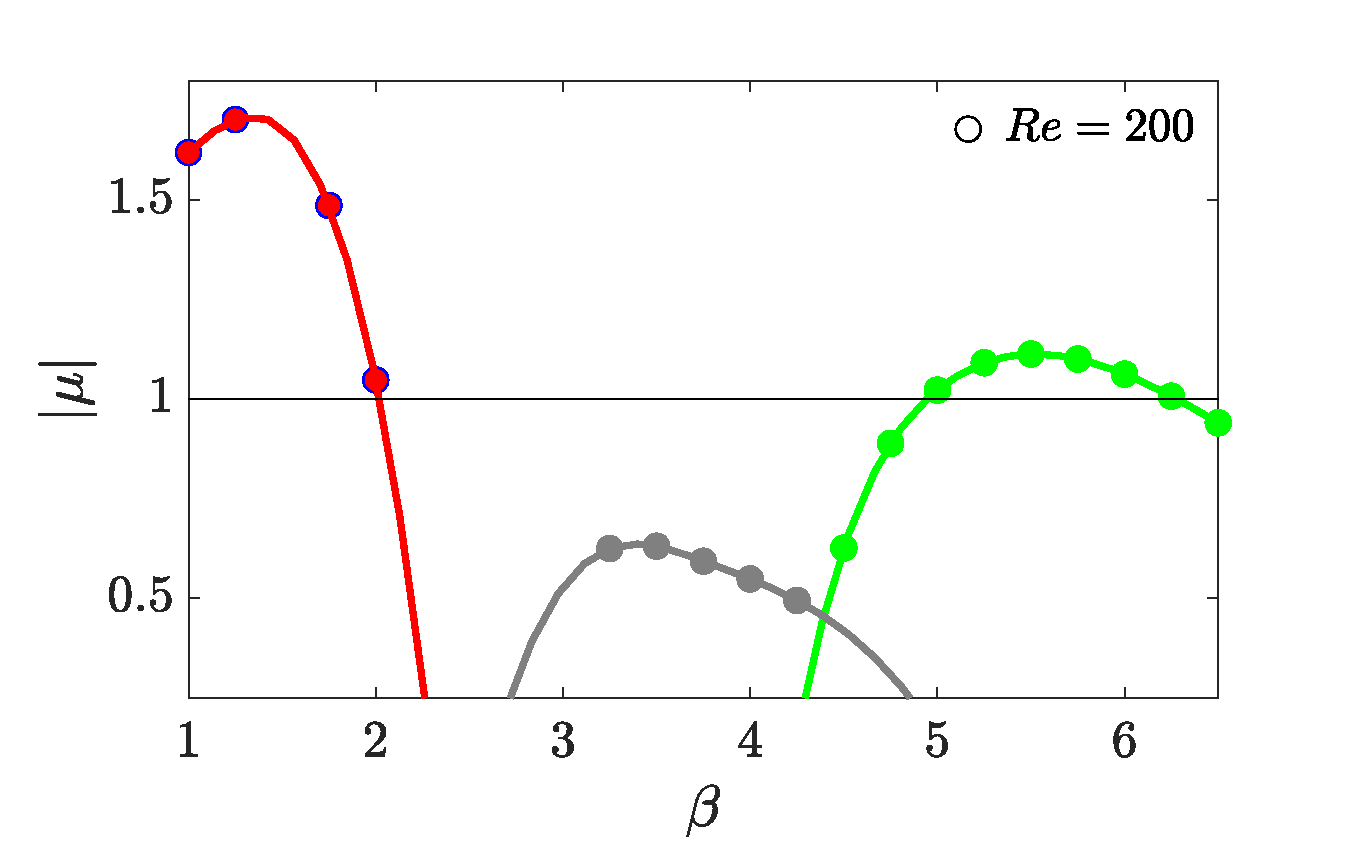
\includegraphics[width=0.49\textwidth]{./fig/AR1s/multipliers_AR1.eps}
  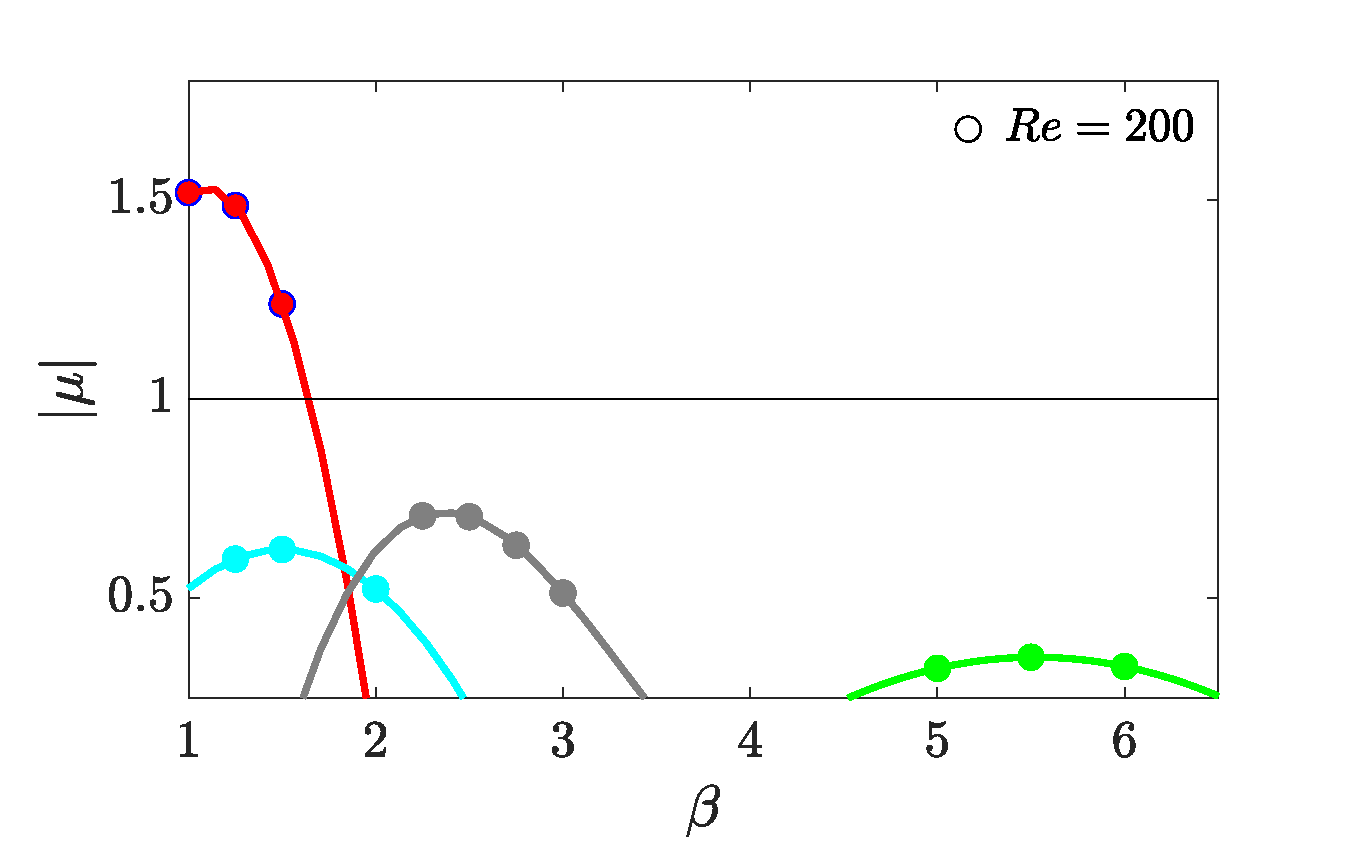
\includegraphics[width=0.49\textwidth]{./fig/AR1s/multipliers_AR1p25.eps}
  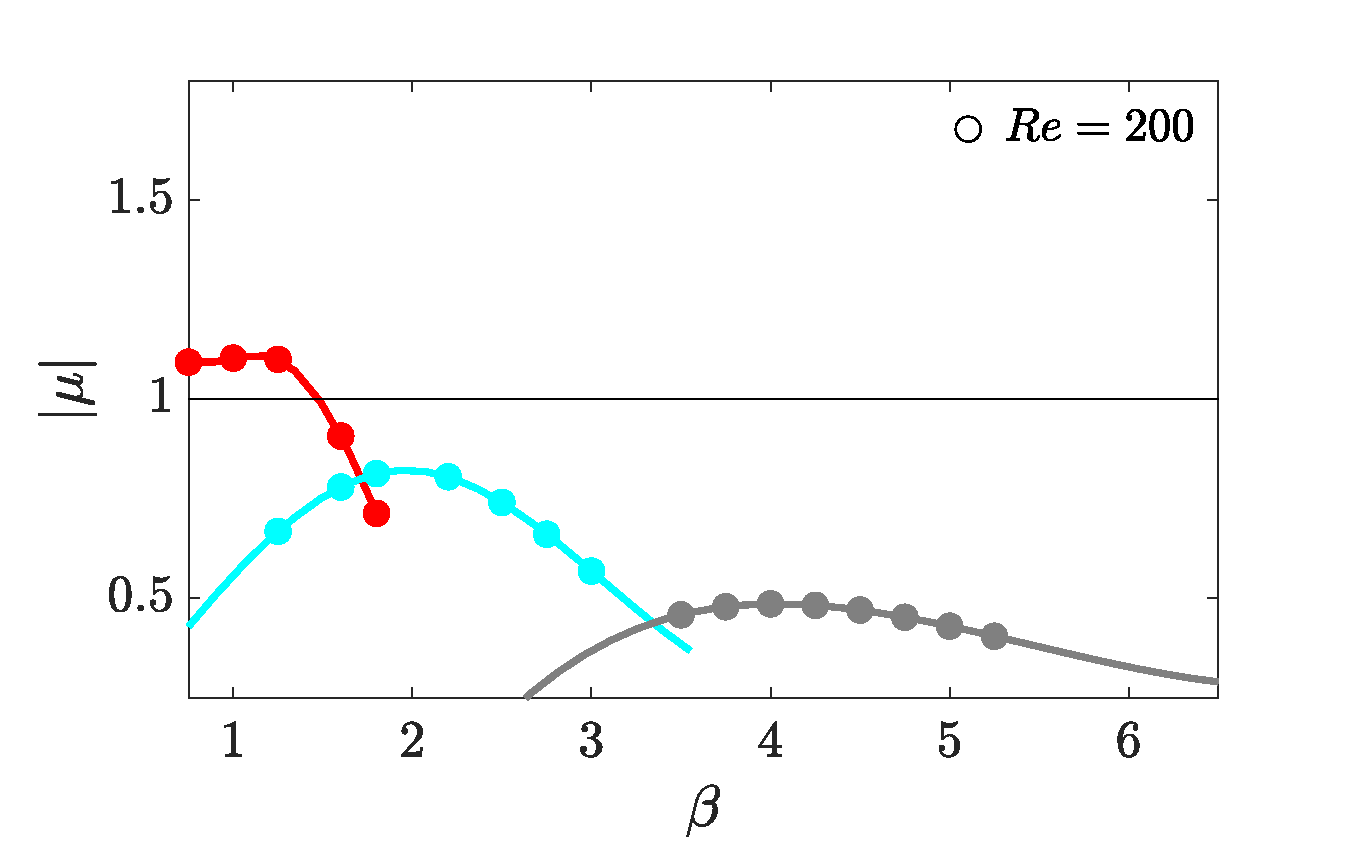
\includegraphics[width=0.49\textwidth]{./fig/AR1s/multipliers_AR1p5.eps}
  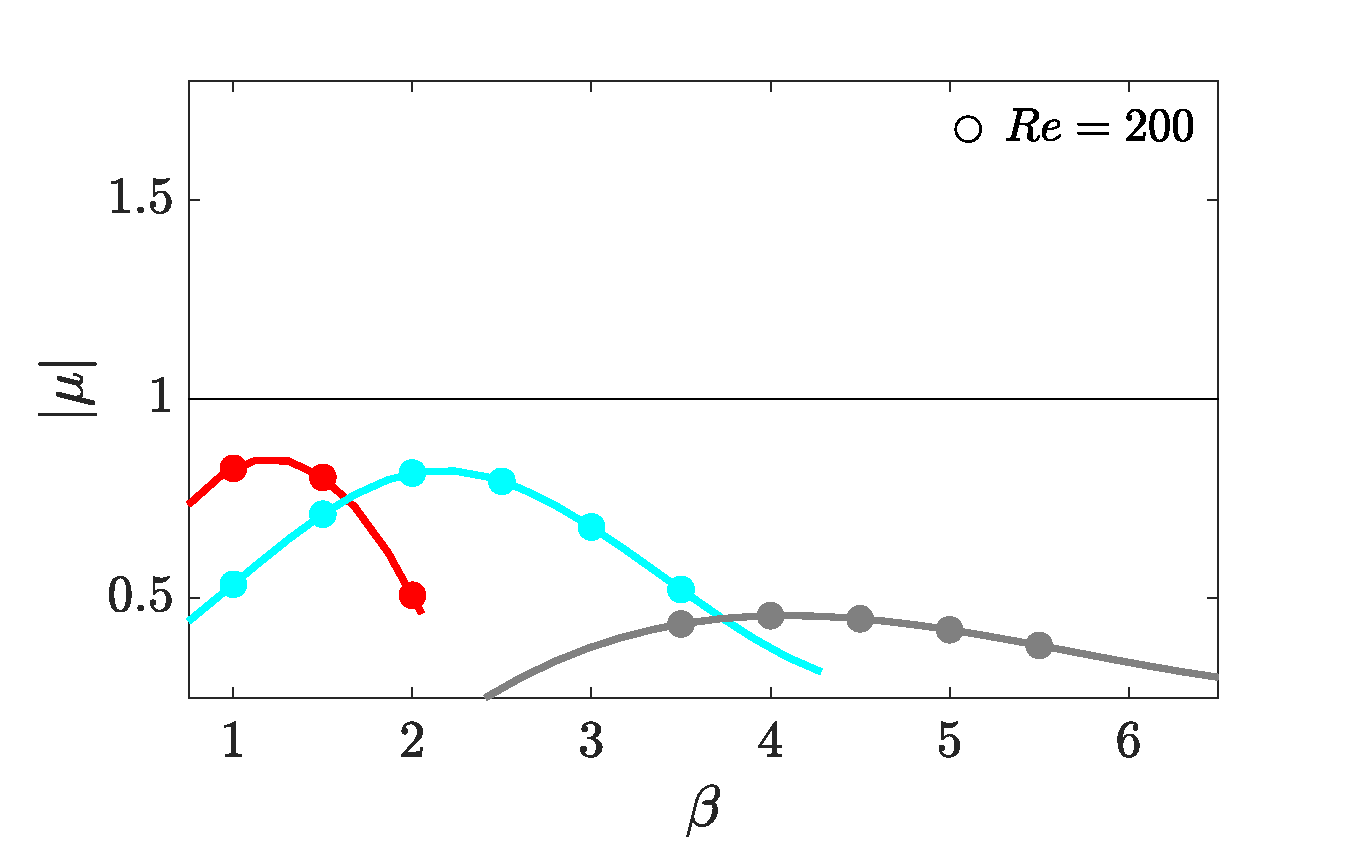
\includegraphics[width=0.49\textwidth]{./fig/AR1s/multipliers_AR1p75.eps} \\
  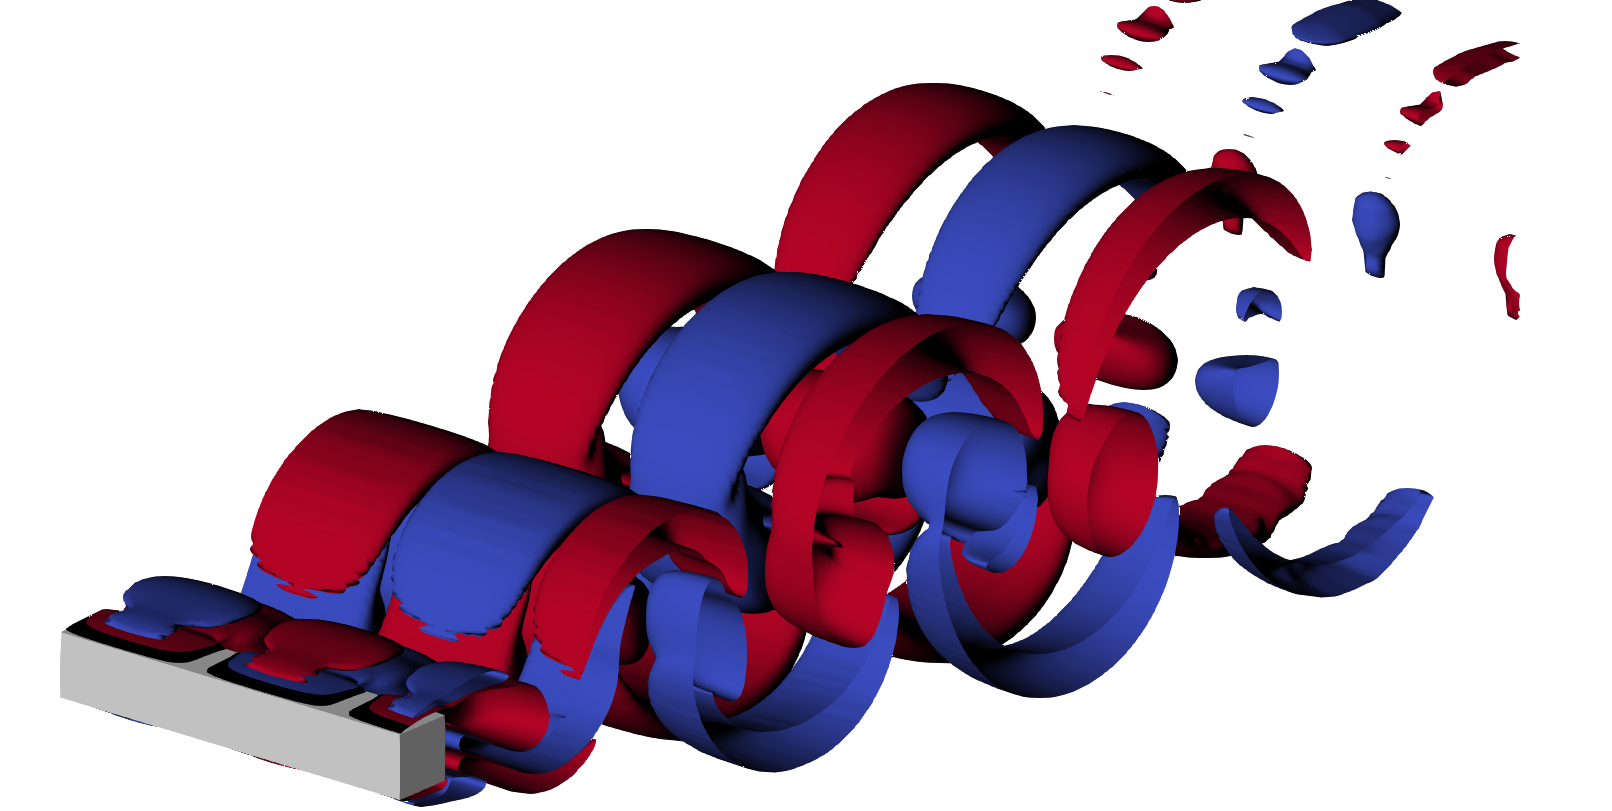
\includegraphics[width=0.49\textwidth]{./fig/AR1s/Floqetmode_beta_1p2_Re200_AR1_A.png}
  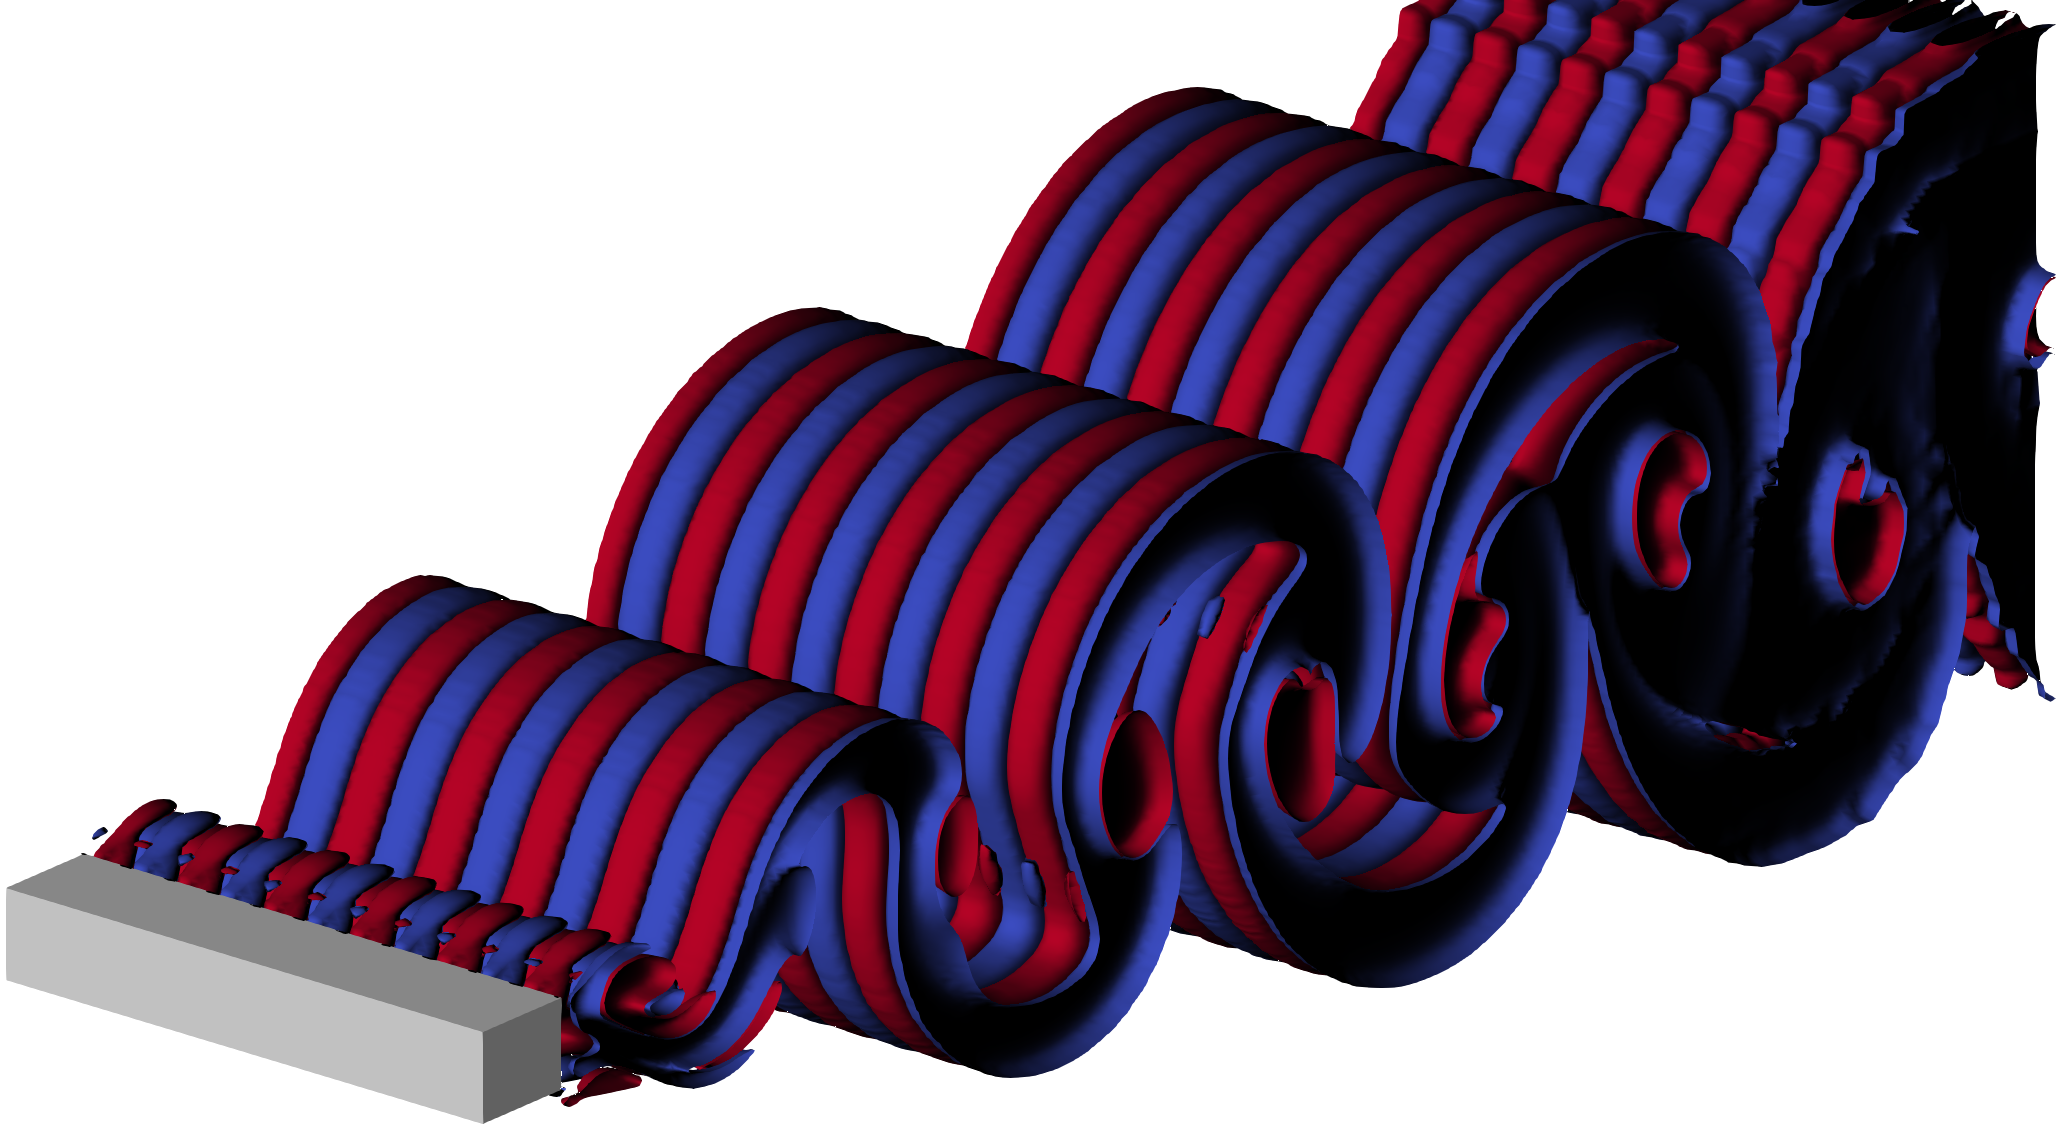
\includegraphics[width=0.49\textwidth]{./fig/AR1s/Floqetmode_beta_5p5_Re200_AR1p25_B.png}
  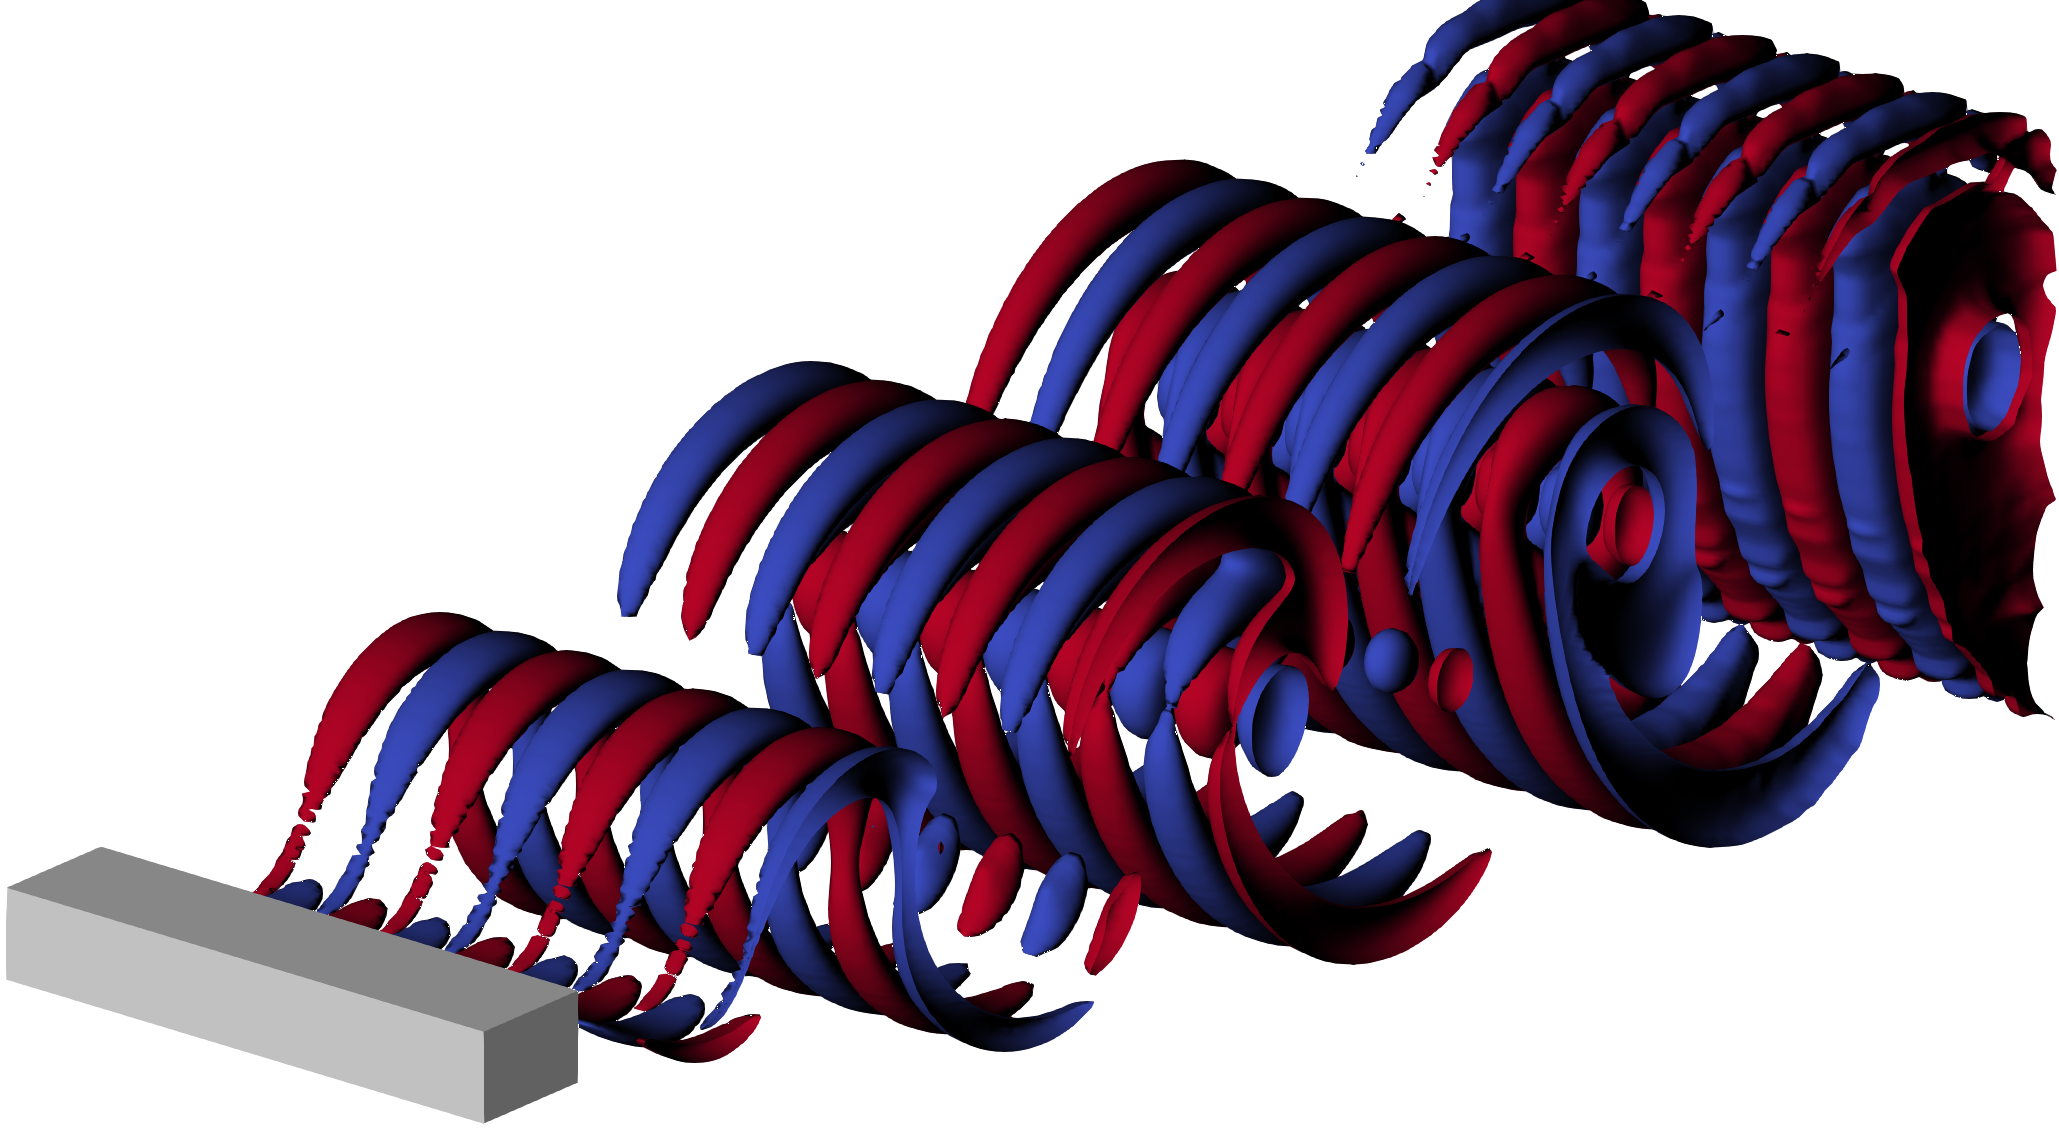
\includegraphics[width=0.49\textwidth]{./fig/AR1s/Floqetmode_beta_3p75_Re200_AR1p5_C.png}
  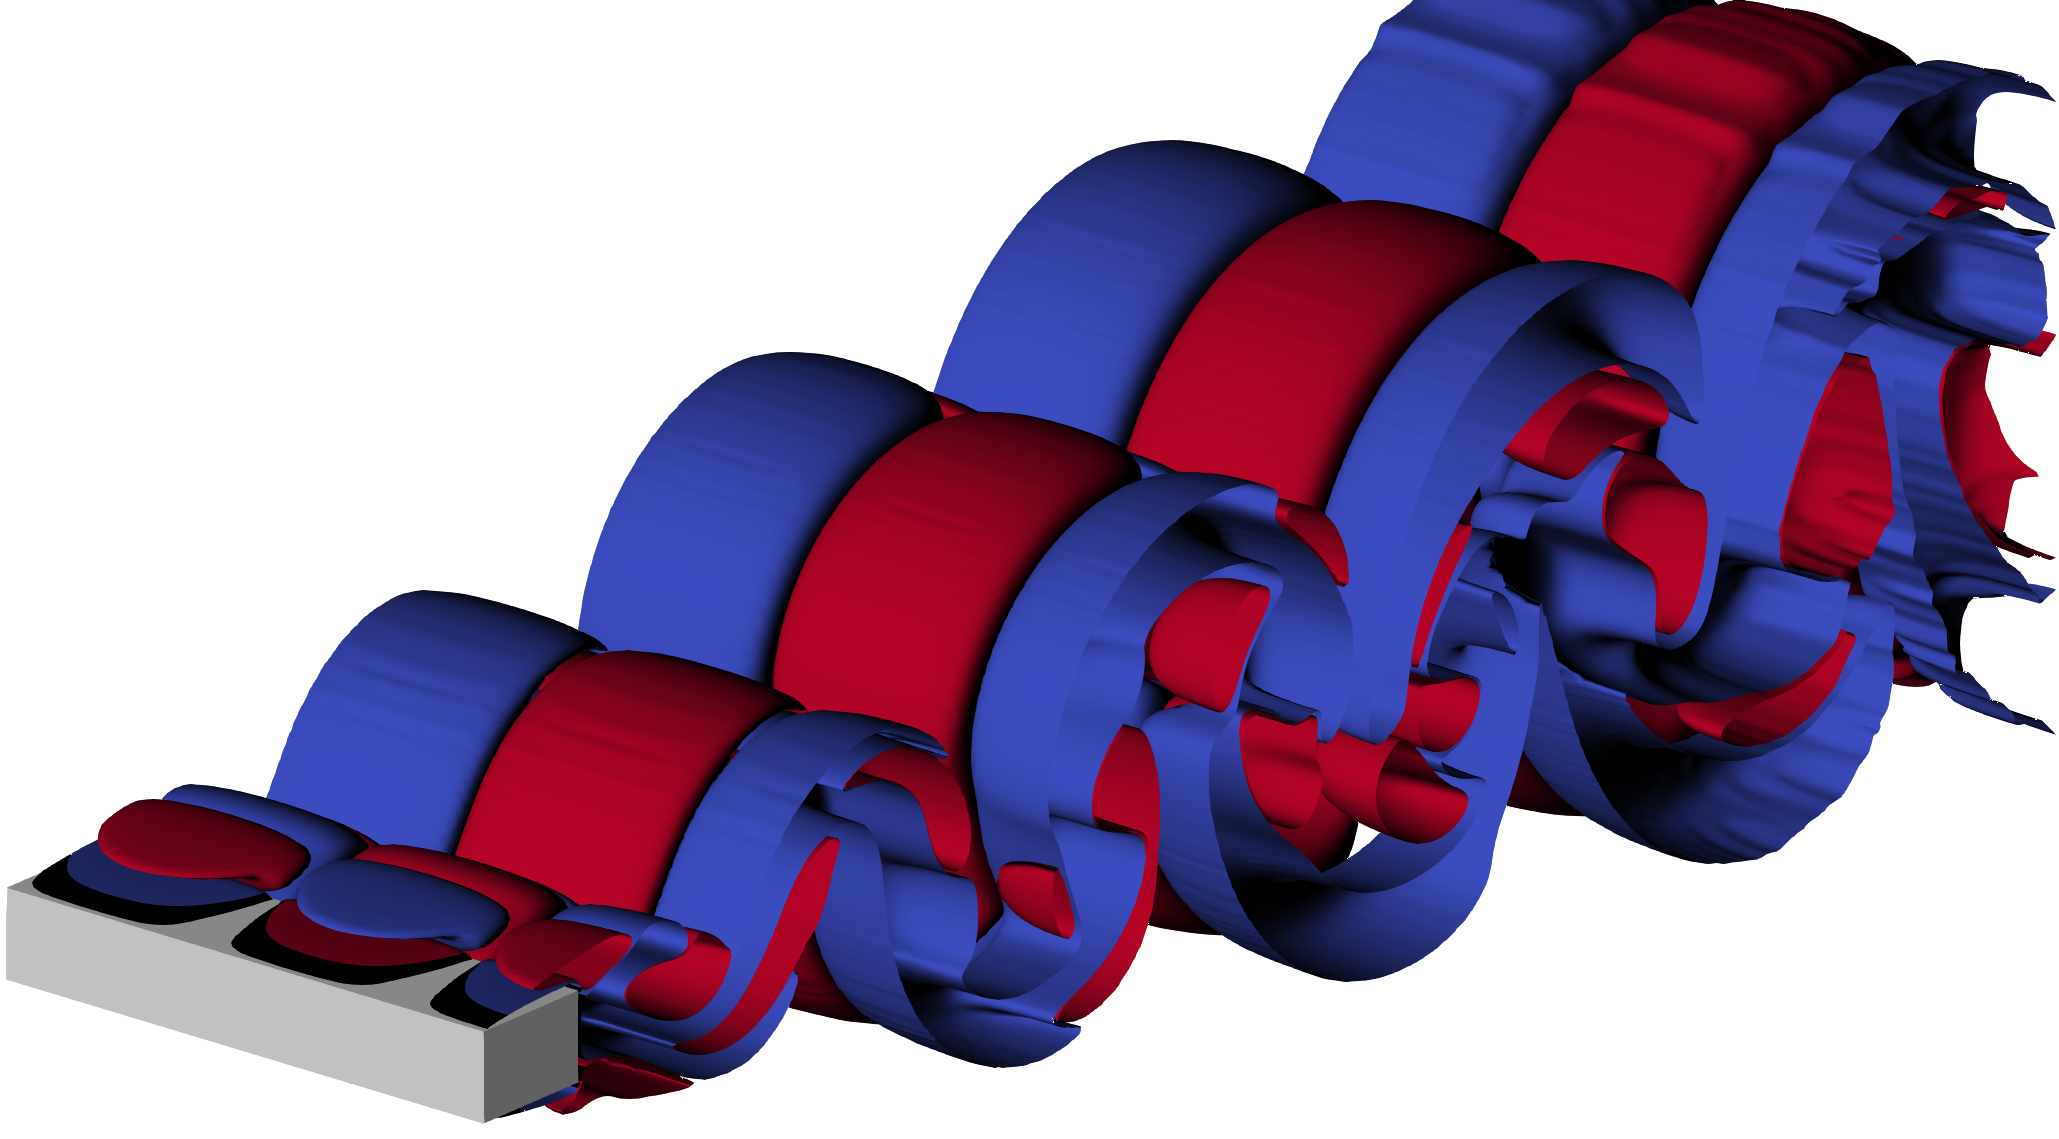
\includegraphics[width=0.49\textwidth]{./fig/AR1s/Floqetmode_beta_1p8_Re200_AR1p5_Bp.png}  
  \caption{Top: multipliers for $\AR=1$, $\AR=1.25$ and $\AR=1.5$ at $Re=200$; the red line refers to mode $A$, the grey line to mode $C$, the green line to mode $B$ and the light blue line refers to mode $B'$. Mode $B'$ has the same spatio-temporal symmetry of mode $B$, but its characteristic wavelength is much smaller, being similar to that of mode $A$. This mode resembles that found for elongated bodies with elliptic leading edge by \cite{ryan-etal-2005}. XX ADD $Re=175$ XX. Bottom: Three-dimensional reconstructions of the Floquet modes for $1 \le \AR \le 1.75$. $(a)$ mode A for $\AR=1$ at $Re=200$ and $\beta=1.2$. $(b)$ mode B for $\AR=1.25$ at $Re=200$ and $\beta=5.5$. $(c)$ mode QP for $\AR=1.5$ at $Re=200$ and $\beta=1.5$. $(d)$ mode B' for $\AR=1.5$ and $\beta=1.8$.}
  \label{fig:mult_AR1_AR1p75}
\end{figure}
%
As mentioned in \S\ref{sec:intro}, for $\AR=1$ three distinct modes become unstable in rapid succession. Mode A first becomes unstable at $Re \approx 175$ with a characteristic wavelength of $\lambda_A \approx 5$ ($\beta_A \approx 1.2$) and the following spatio-temporal symmetry 
%
\begin{equation}
  \hat{\omega}_x(x,y,\beta,t) = - \hat{\omega}_x(x,-y,\beta,t+/2)
\end{equation}
%
Mode B becomes unstable at $Re \approx 200$, has a characteristic wavelength $\lambda_B \approx 1$ ($\beta_B \approx 5.8$) and satisfies the symmetry:
%
\begin{equation}
  \hat{\omega}_x(x,y,\beta,t) = + \hat{\omega}_x(x,-y,\beta,t+T/2).
\end{equation}
%
Finally, mode QP becomes unstable at the higher $Re \approx 230$ with a characteristic wavelength of $\lambda_{QP} \approx 2.7$ ($\beta_{QP} \approx 2.3$). These results are in excellent agreement with our findings shown in figure~\ref{fig:mult_AR1_AR1p75}$(a)$, providing a validation of our numerical approach.

Figure~\ref{fig:mult_AR1_AR1p75} illustrates the effect of increasing the aspect ratio. As $\AR$ increases, the onset of secondary instabilities is progressively delayes: fixing $Re$ our results show a consistent decrease inthe modulus of the Floquet multipliers associated with the three known modes, indicating a more stable base flow for longer bodies. Quantitativley, the critical Reynolds number increases from $Re_{c2} \approx 175$ for $\AR=1$ to approximately $Re_{c2} =200-225$ for $\AR=1.75$. This trend aligns with the delyed onset of the primary instability reported by \cite{chiarini-quadrio-auteri-2021}. Despite the stabilising effect, the sequence of bifurcations remains essentially unchanged for $1 \le \AR \le 1.75$, with mode A becoming unstable first, followed by mode B. The characteristic wavelengths of these modes exhibit only martinal variations with $\AR$, consistent with the findings of \cite{choi-yang-2014} for $\AR<1$.

In addition to the three established modes, a new mode, denoted B', emergest for $\AR>1$. Mode B' shares the same spatio-temporal symmetry as mode B, but is characterised by a significantly longer wavelength, comparable to that of mode A; see figure \ref{fig:modes_AR1_AR1p75}. A mode with similar features --- both in wavelength and symmetry --- was previously reported by \cite{ryan-etal-2006} in the wake of elongated bodies with streamlined LE and blunt TE. However, within the parameter range considered here, mode B' remains stable.

\begin{figure}
  \centering
  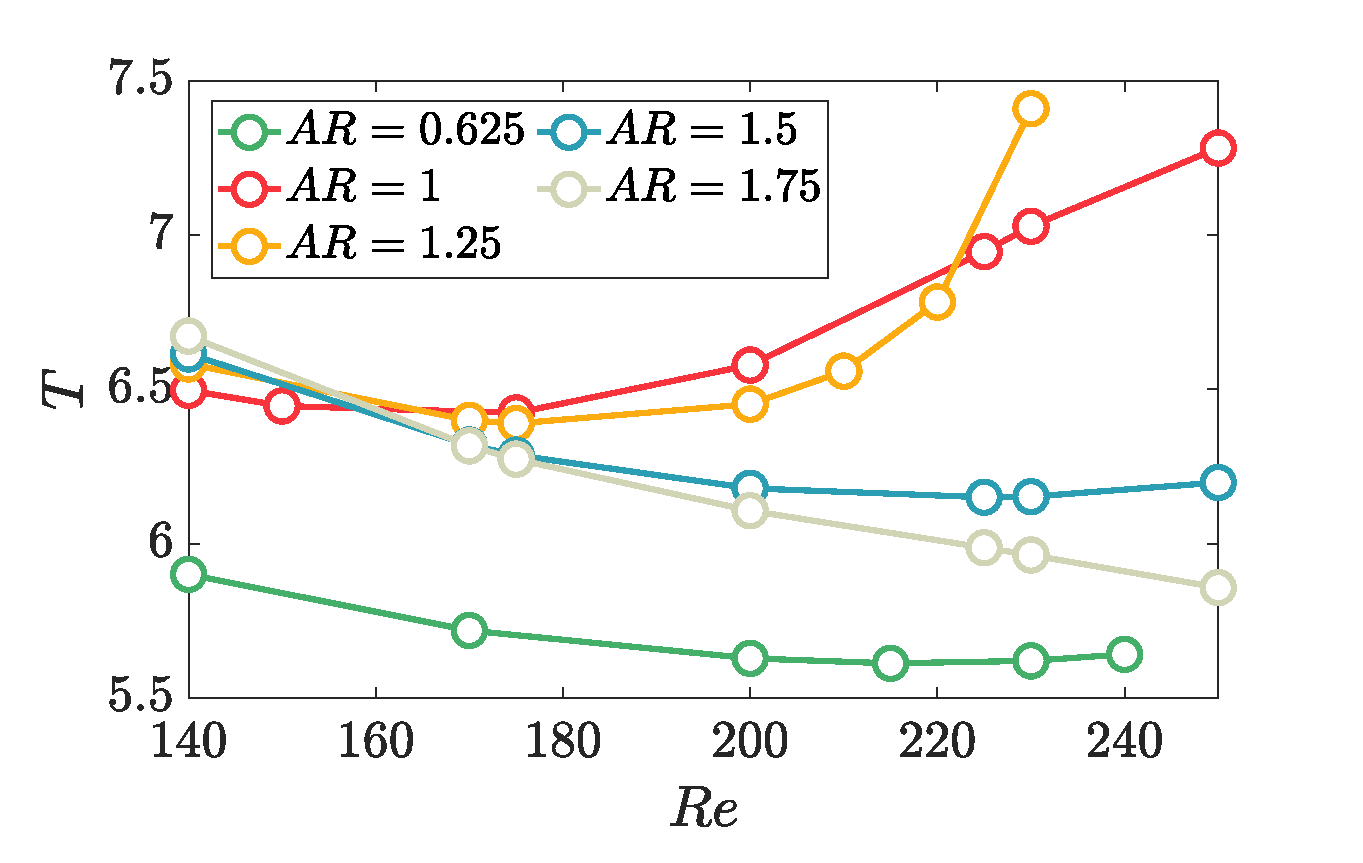
\includegraphics[width=0.49\textwidth]{./fig/AR1s/T_Re.eps}
  \caption{Period of the limit cycle for $1 \le \AR \le 1.75$ as a function of the Reynolds number. XX ADD (i) PANEL WITH DEPENDENCE OF $T$ ON $\AR$ FOR A SELECTED $Re$. (ii) PANEL WITH DEPENDENCE OF THE AERODYNAMIC FORCES on $\AR$ and $Re$. (iii) PANEL WITH DEPENDENCE OF MEAN-FLOW QUANTITIES ON $\AR$ and $Re$. XX}
  \label{fig:T_Re_small}
\end{figure}
%
For $Re>Re_{c2}$ the stability scenario becomes more complex, as the influence of $Re$ on the base-flow topology varies with $\AR$. This trend is clearly illustrated in figure \ref{fig:T_Re_small}, which shows the dependence of the base-flow shedding period $T$ on both $Re$ and $\AR$. For the shortest and logest bodies, $T$ exhibits only minor variations with increase $Re$: it increases by approximately $xx\%$ for $\AR =1$ and decreases by about $xx\%$ for $\AR=1.75$. In contrast, intermediated aspect ratios ($\AR=1.25$) show a mouch stornger dependence on $Re$. Here, $T$ increases significantly with $Re$ rising from $T \approx 6.5$ at $Re \le 210$ to $T \approx 9$ at $Re \ge 250$. This shift reflects changes in the base-flow topology and coincides wit the emergence of new instability modes. The differing sensitivity of the base-flow to $Re$ is further quantified in figure~\ref{fig:T_Re_small}(c-d) which shows the aerodynamics forces and characterstic mean-flow length scales.

XX GUARDARE IL CAMPO MEDIO. FACCIAMO STABILITA DEL CAMPO MEDIO PER VEDERE SE CAPIAMO QUALCOSA RIGUARDO AL DIVERSO SHEDDING? XX


\begin{figure}
  \centering
  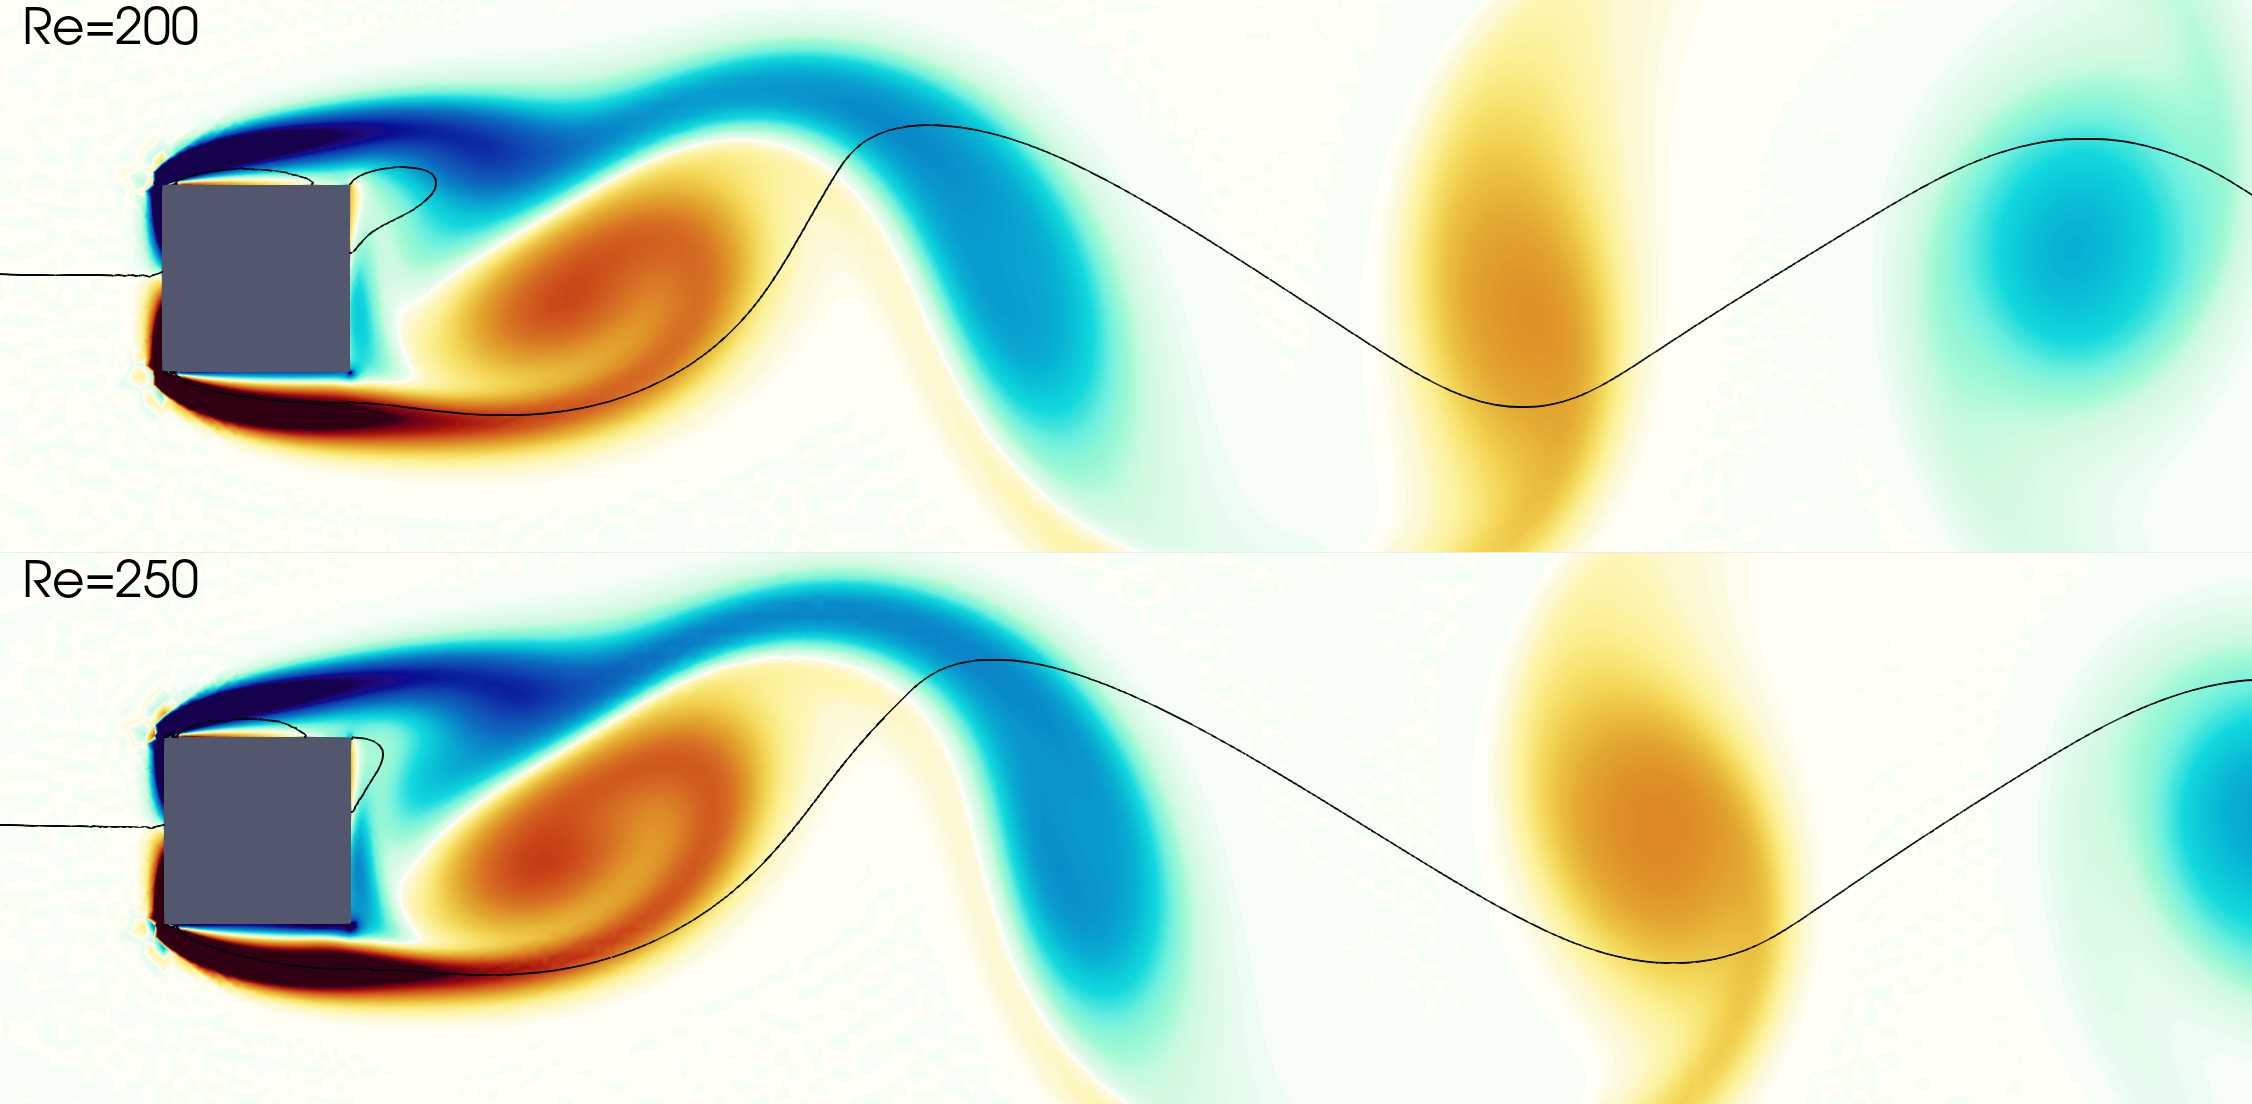
\includegraphics[width=0.49\textwidth]{./fig/AR1/snap/snap.0000.png}
  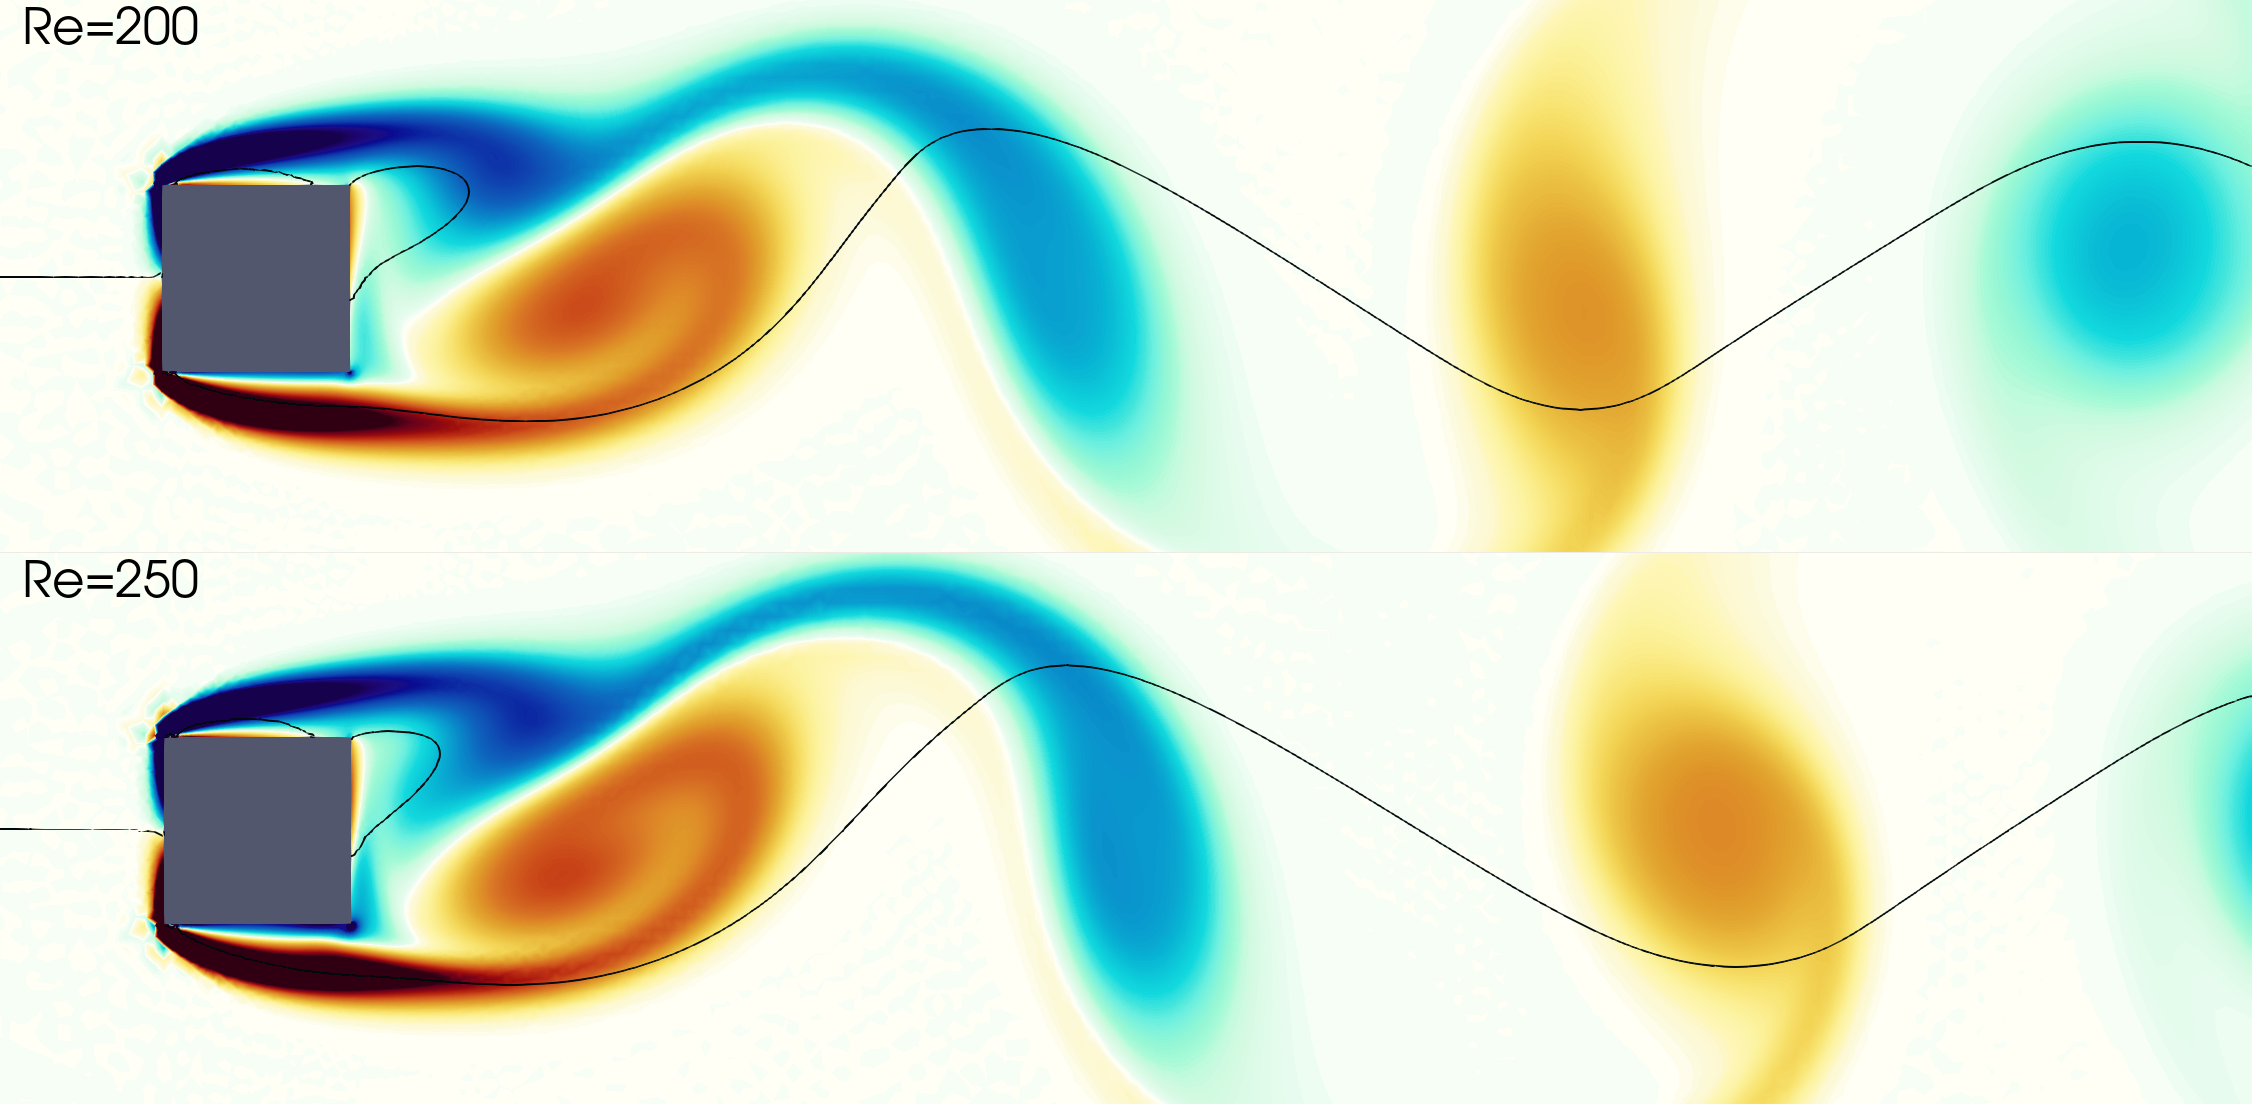
\includegraphics[width=0.49\textwidth]{./fig/AR1/snap/snap.0005.png}
  \begin{tikzpicture}
  \draw (-10,2) -- (8,2);
  \end{tikzpicture}
  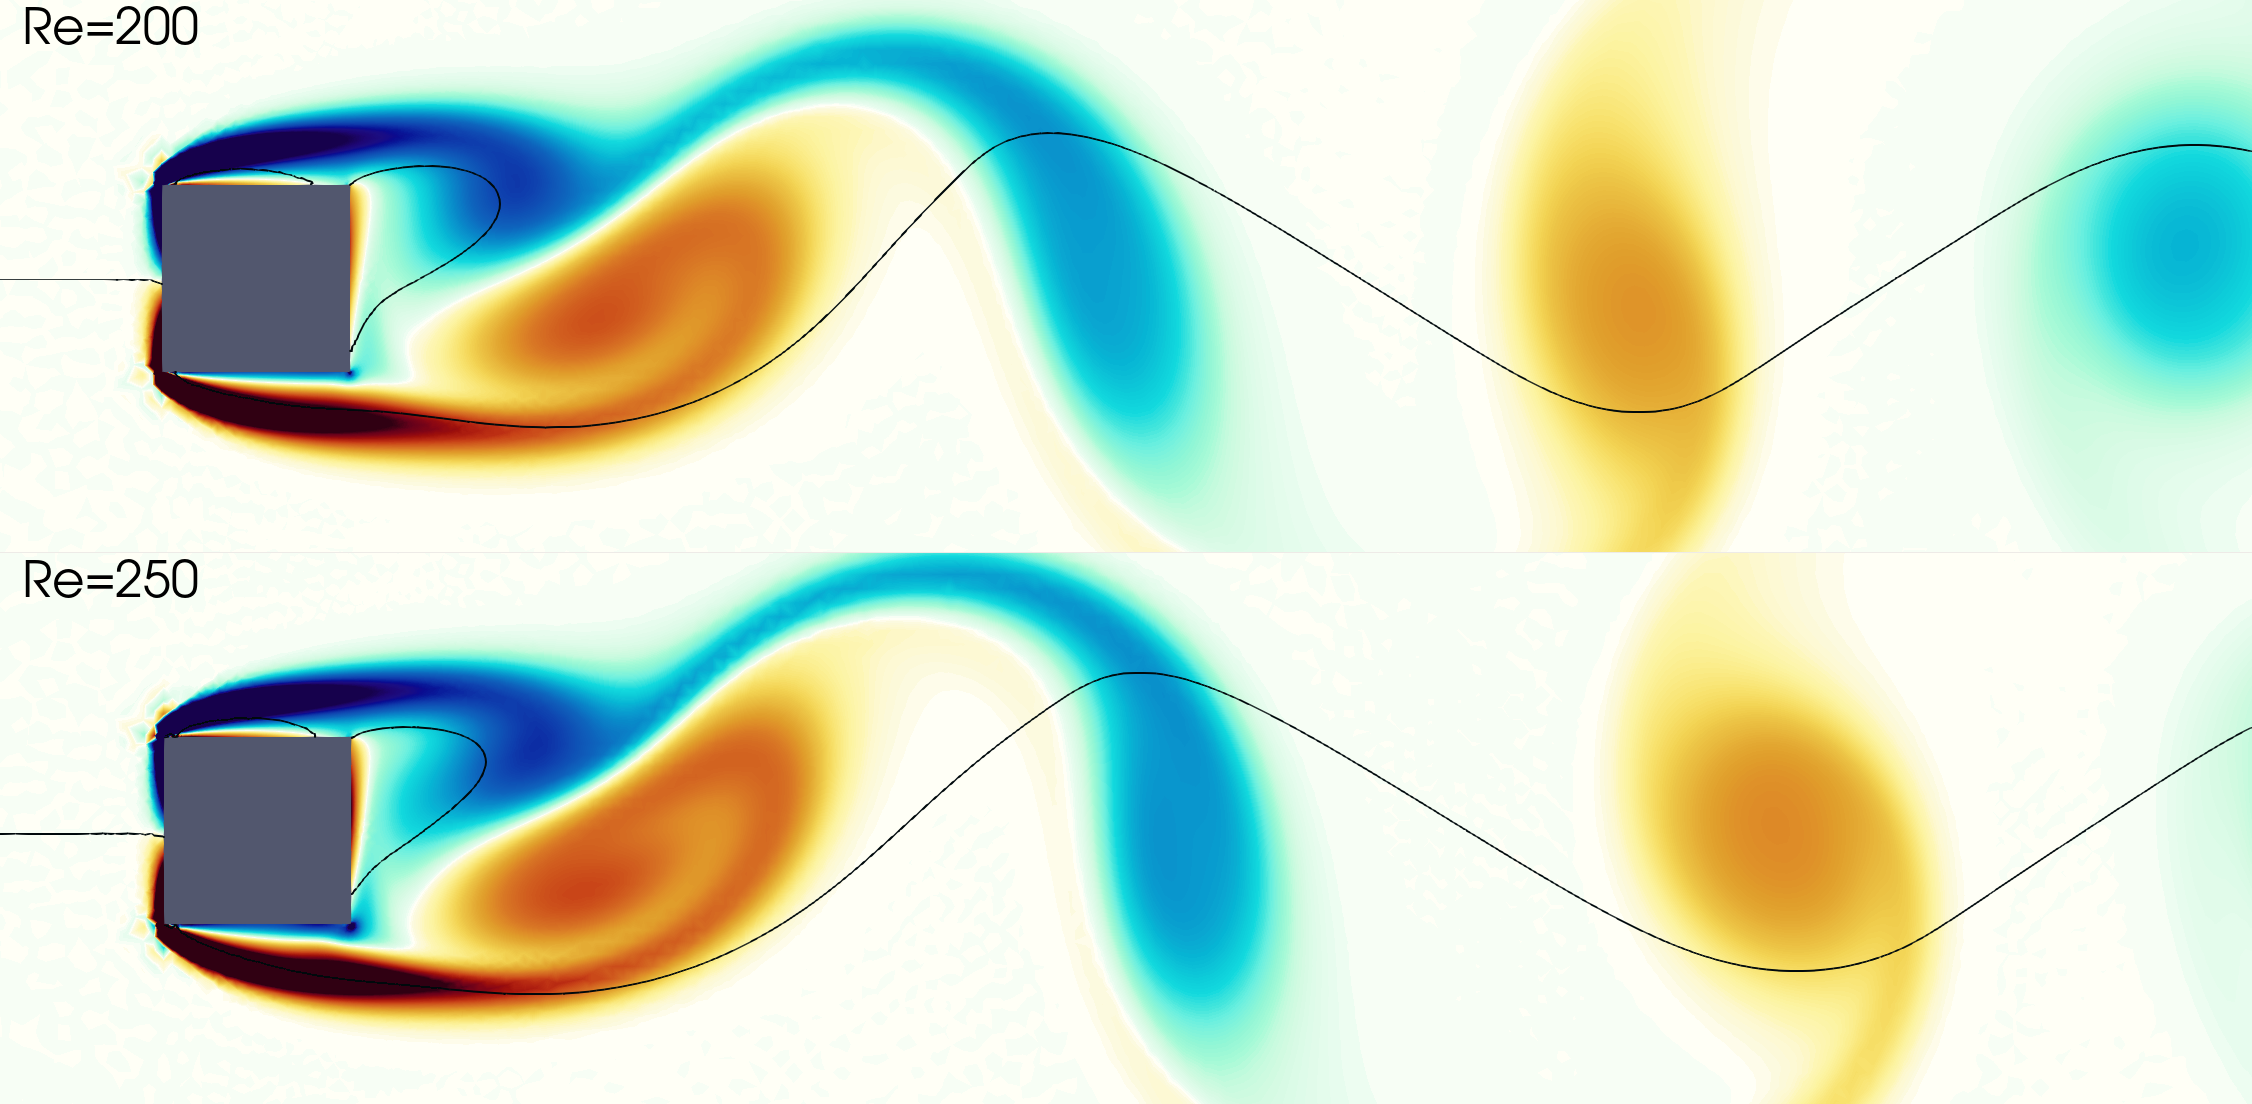
\includegraphics[width=0.49\textwidth]{./fig/AR1/snap/snap.0010.png}
  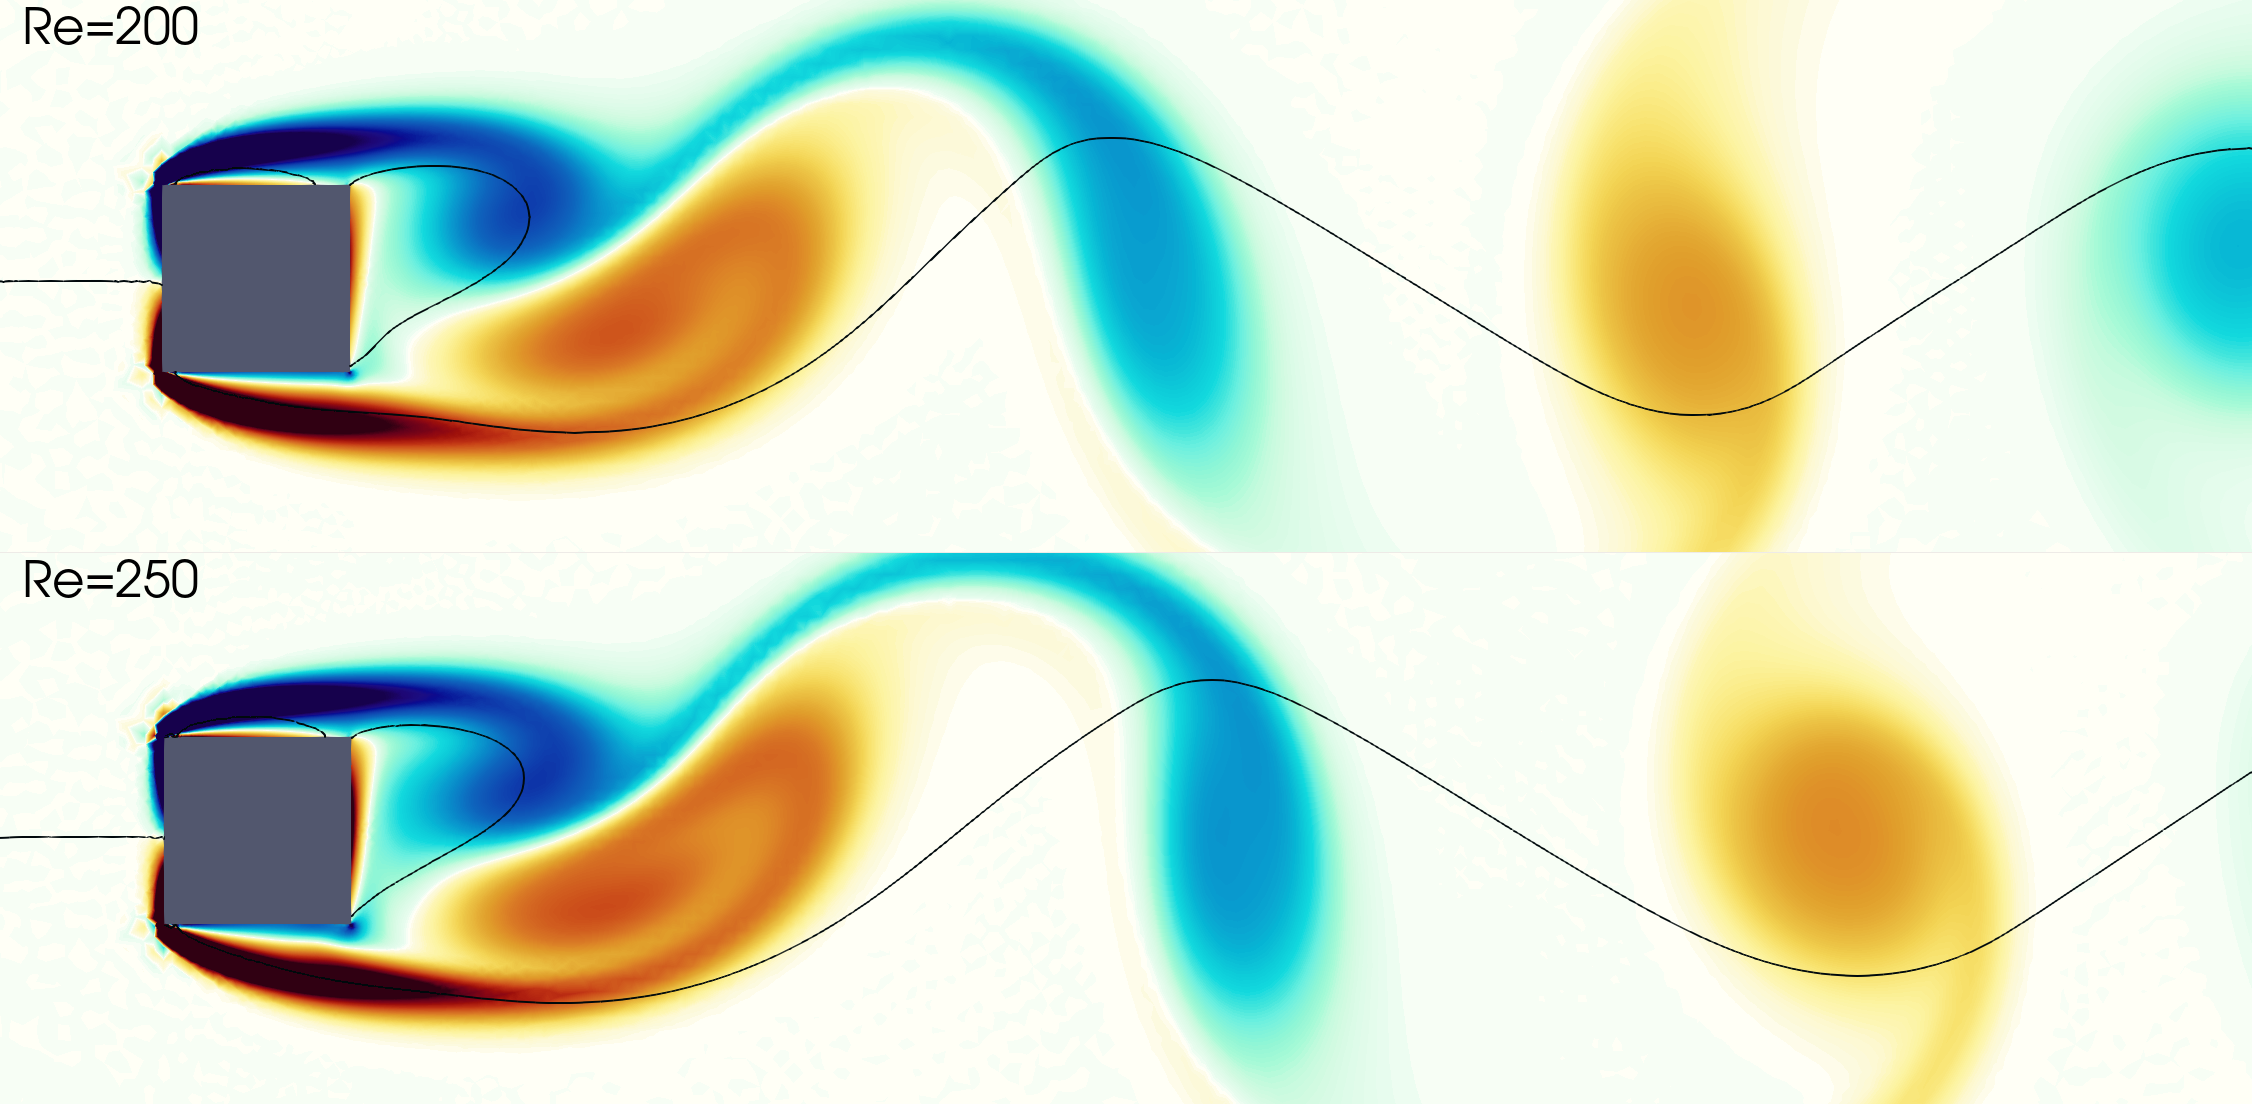
\includegraphics[width=0.49\textwidth]{./fig/AR1/snap/snap.0015.png}
  \begin{tikzpicture}
  \draw (-10,2) -- (8,2);
  \end{tikzpicture}
  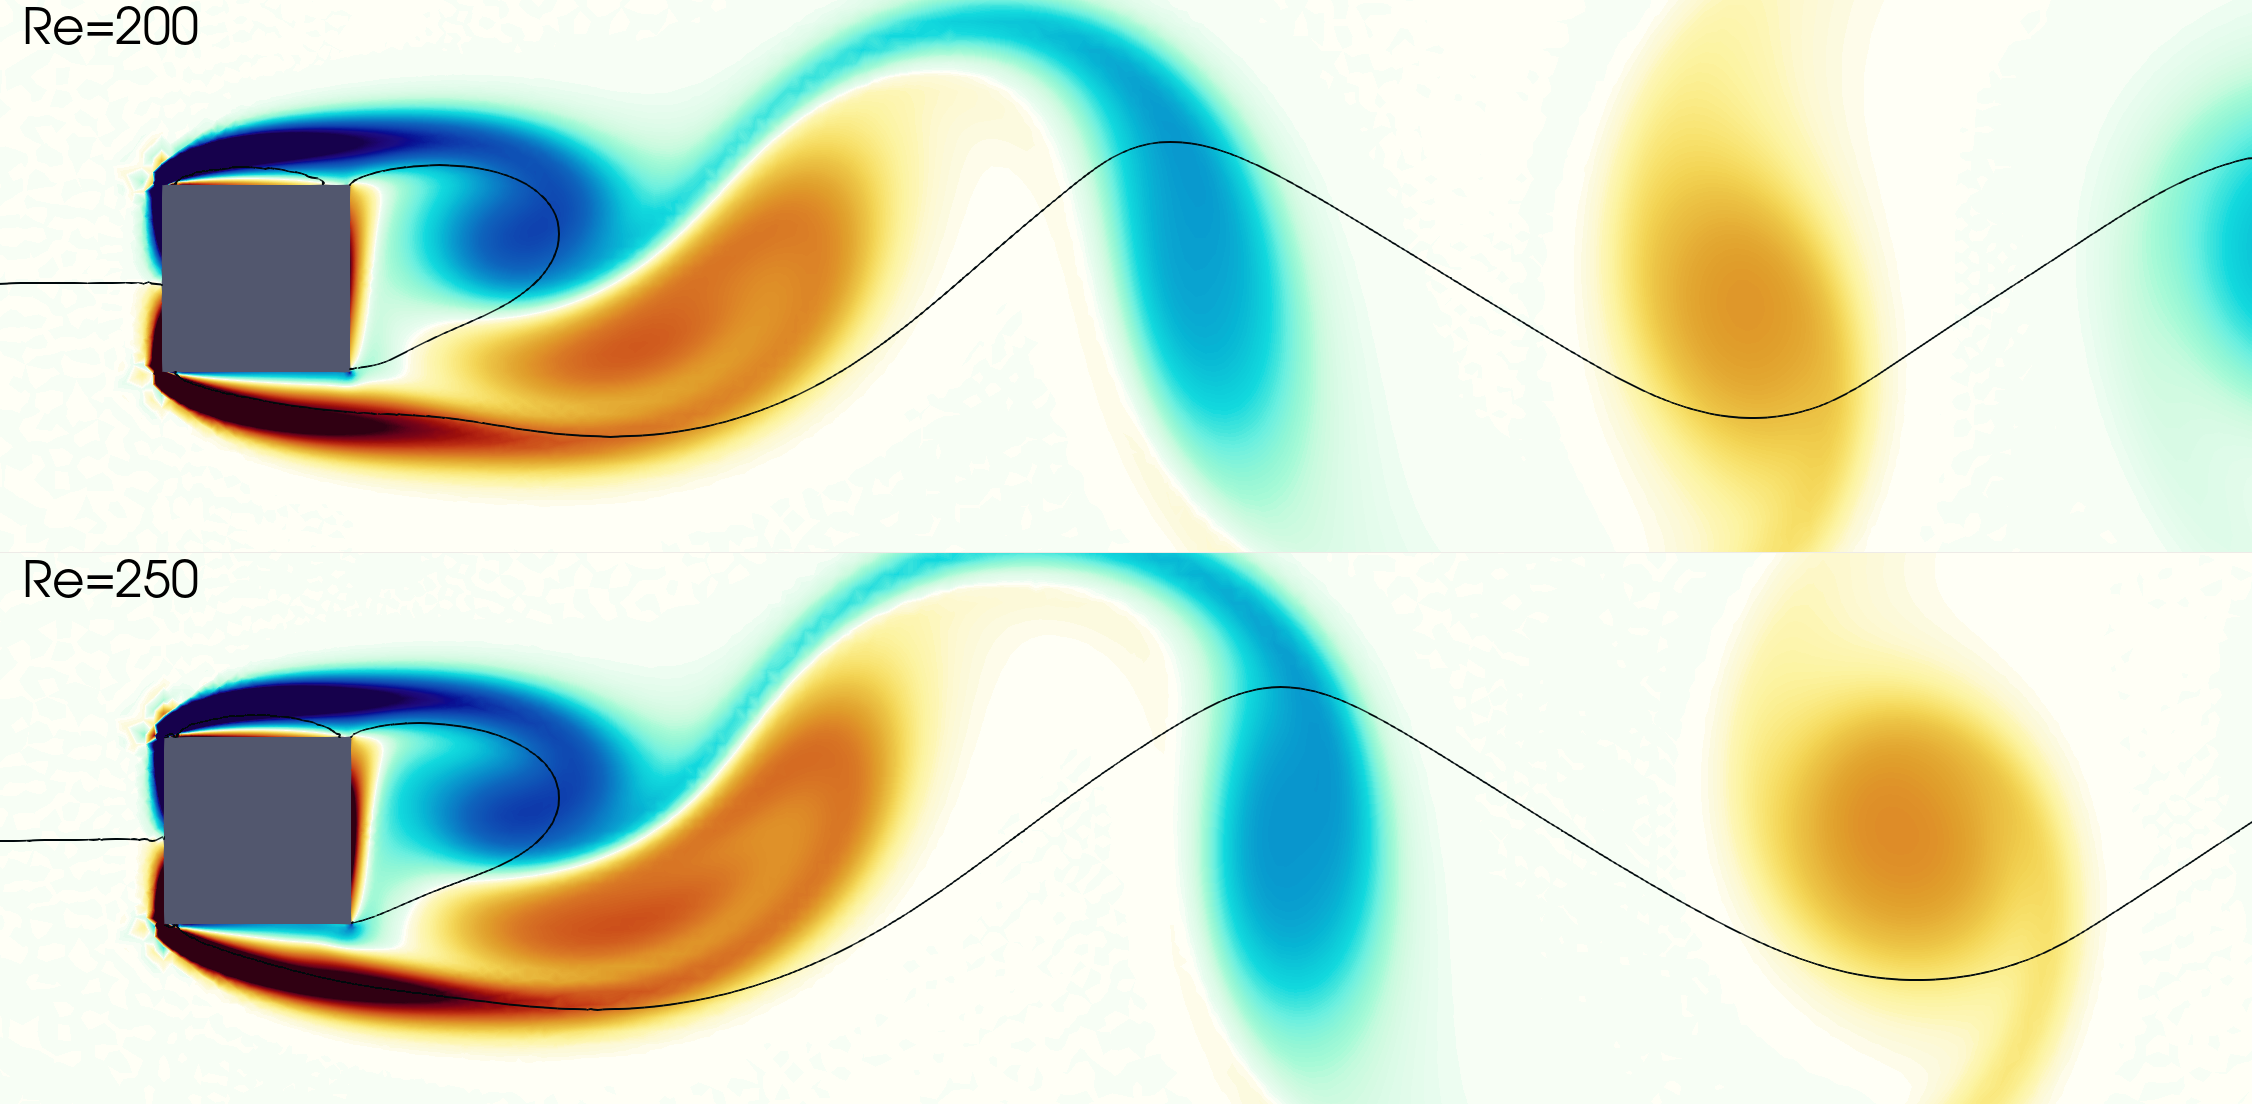
\includegraphics[width=0.49\textwidth]{./fig/AR1/snap/snap.0020.png}
  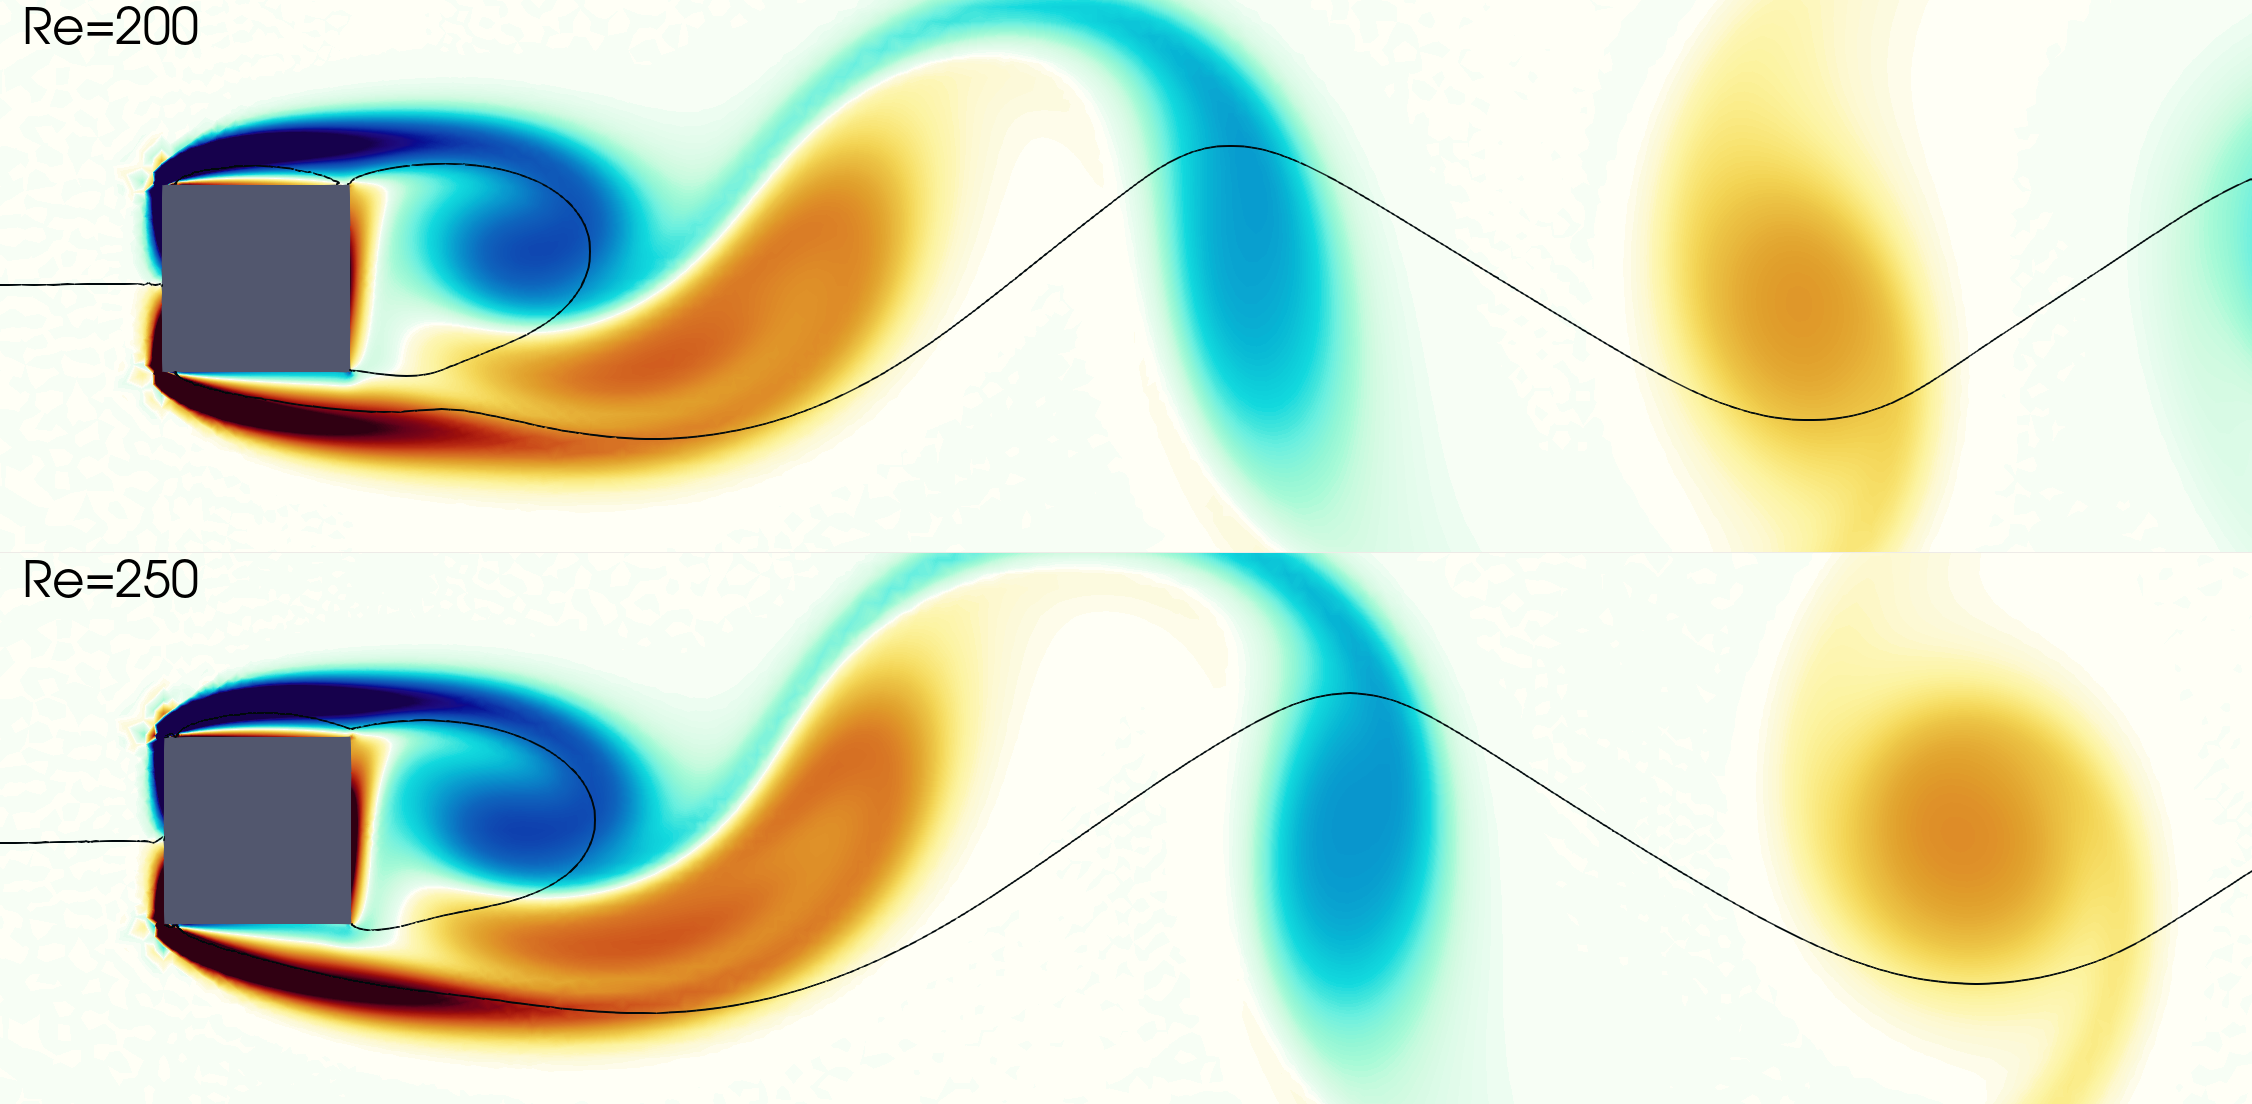
\includegraphics[width=0.49\textwidth]{./fig/AR1/snap/snap.0025.png}
  \begin{tikzpicture}
  \draw (-10,2) -- (8,2);
  \end{tikzpicture}
  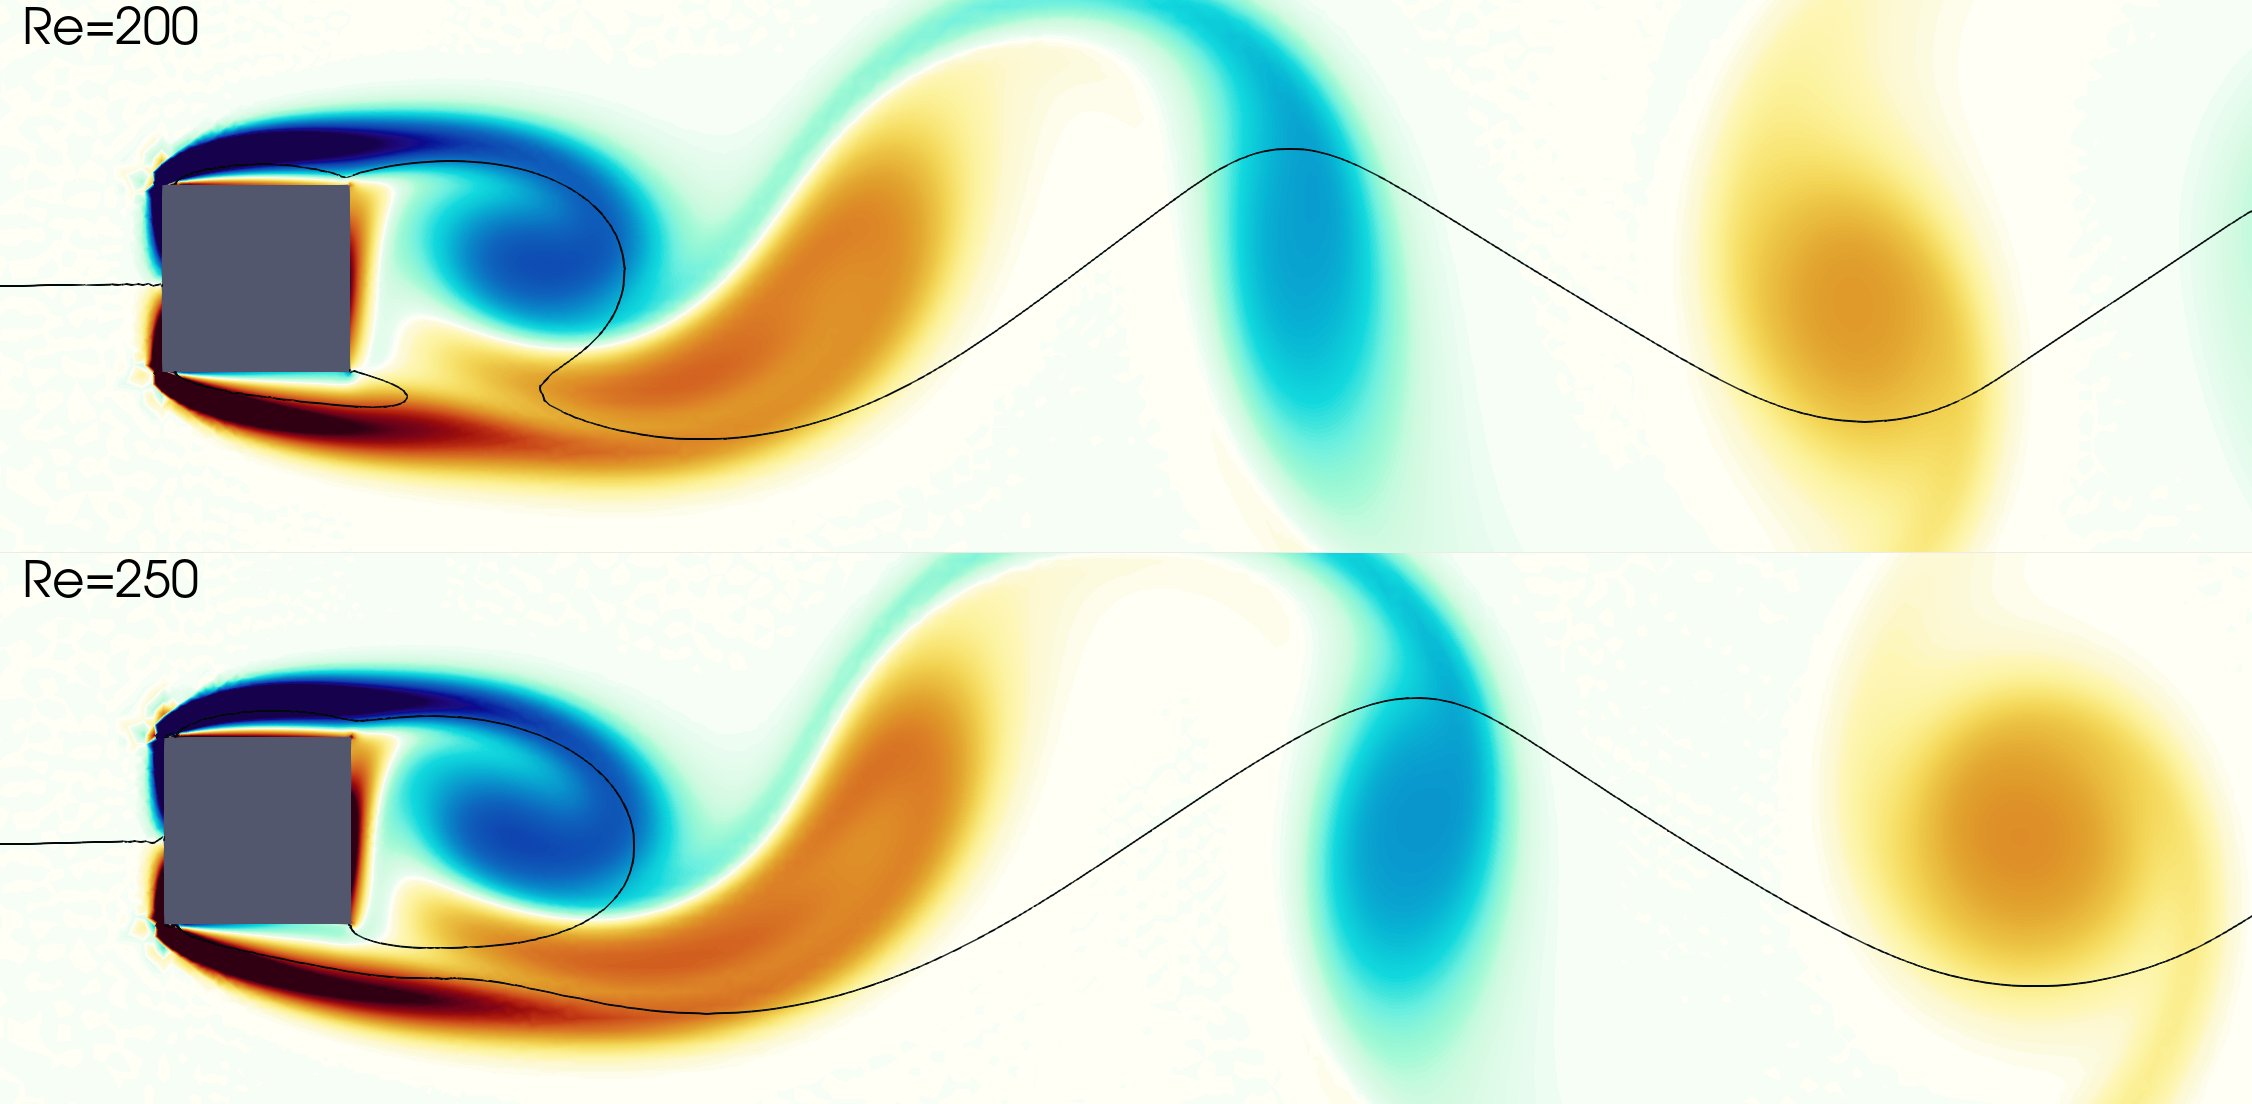
\includegraphics[width=0.49\textwidth]{./fig/AR1/snap/snap.0030.png}
  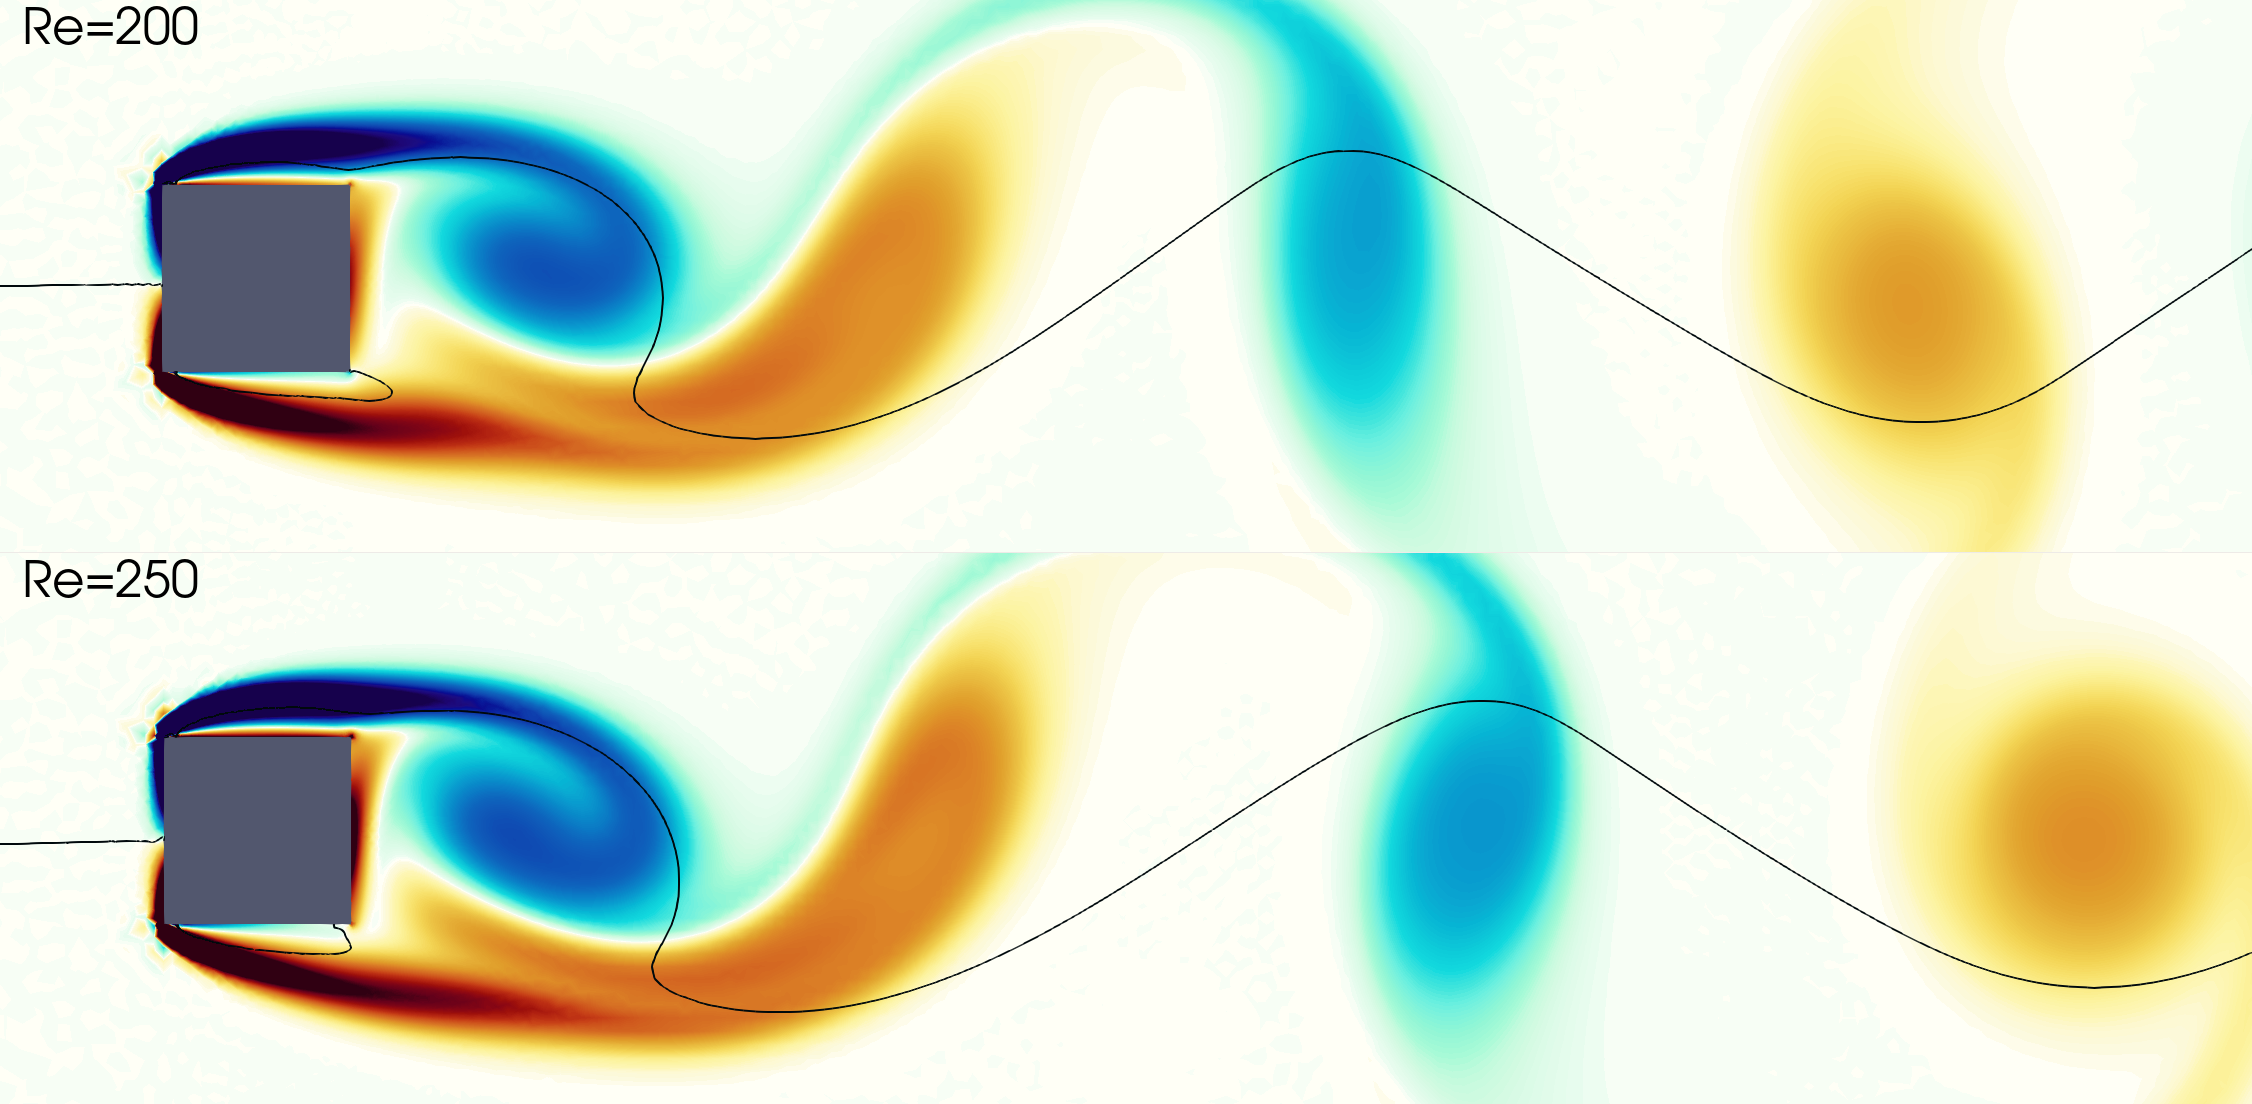
\includegraphics[width=0.49\textwidth]{./fig/AR1/snap/snap.0035.png}
  \begin{tikzpicture}
  \draw (-10,2) -- (8,2);
  \end{tikzpicture}
  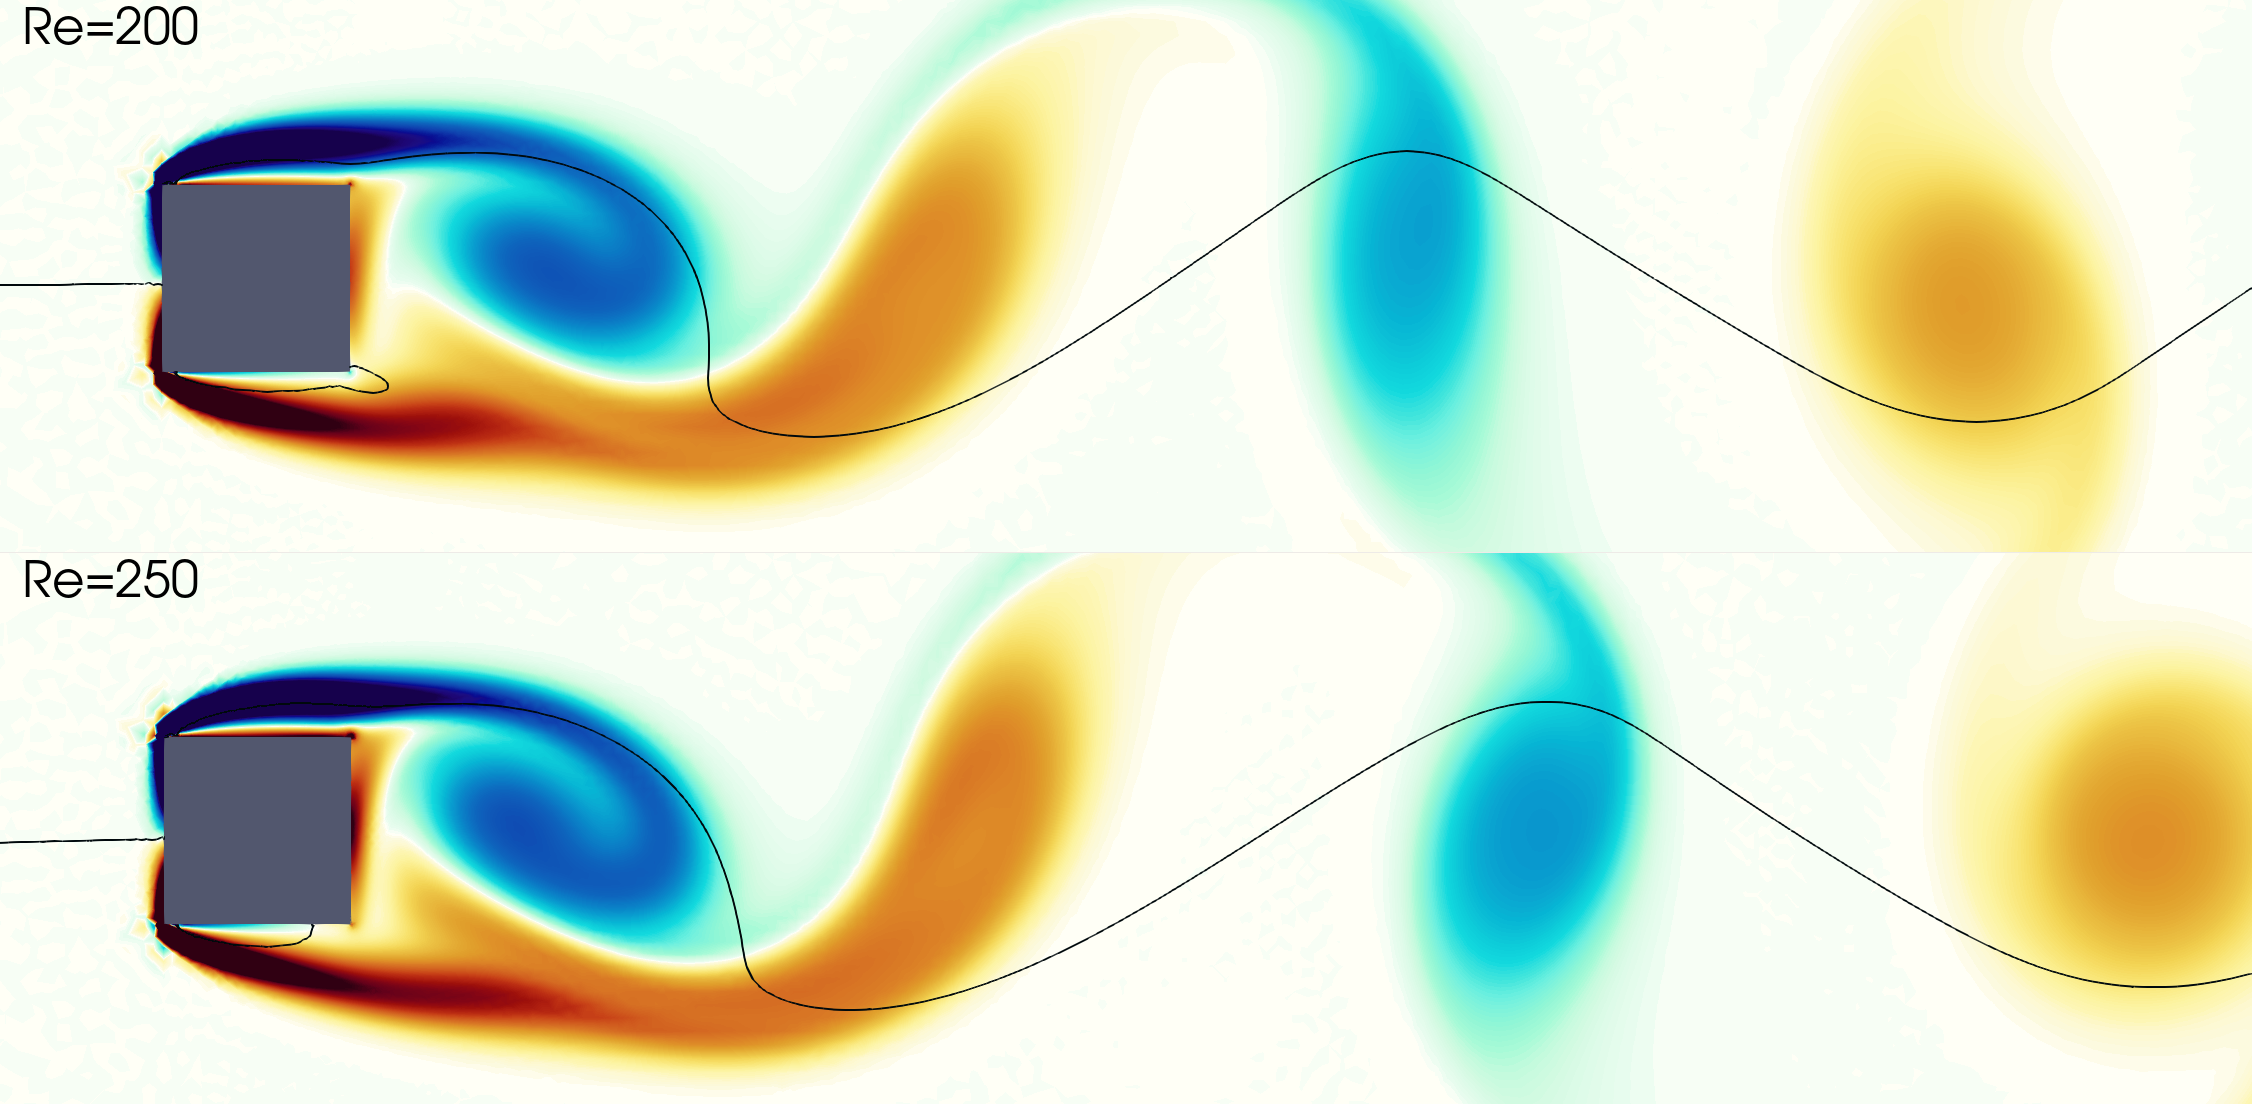
\includegraphics[width=0.49\textwidth]{./fig/AR1/snap/snap.0040.png}
  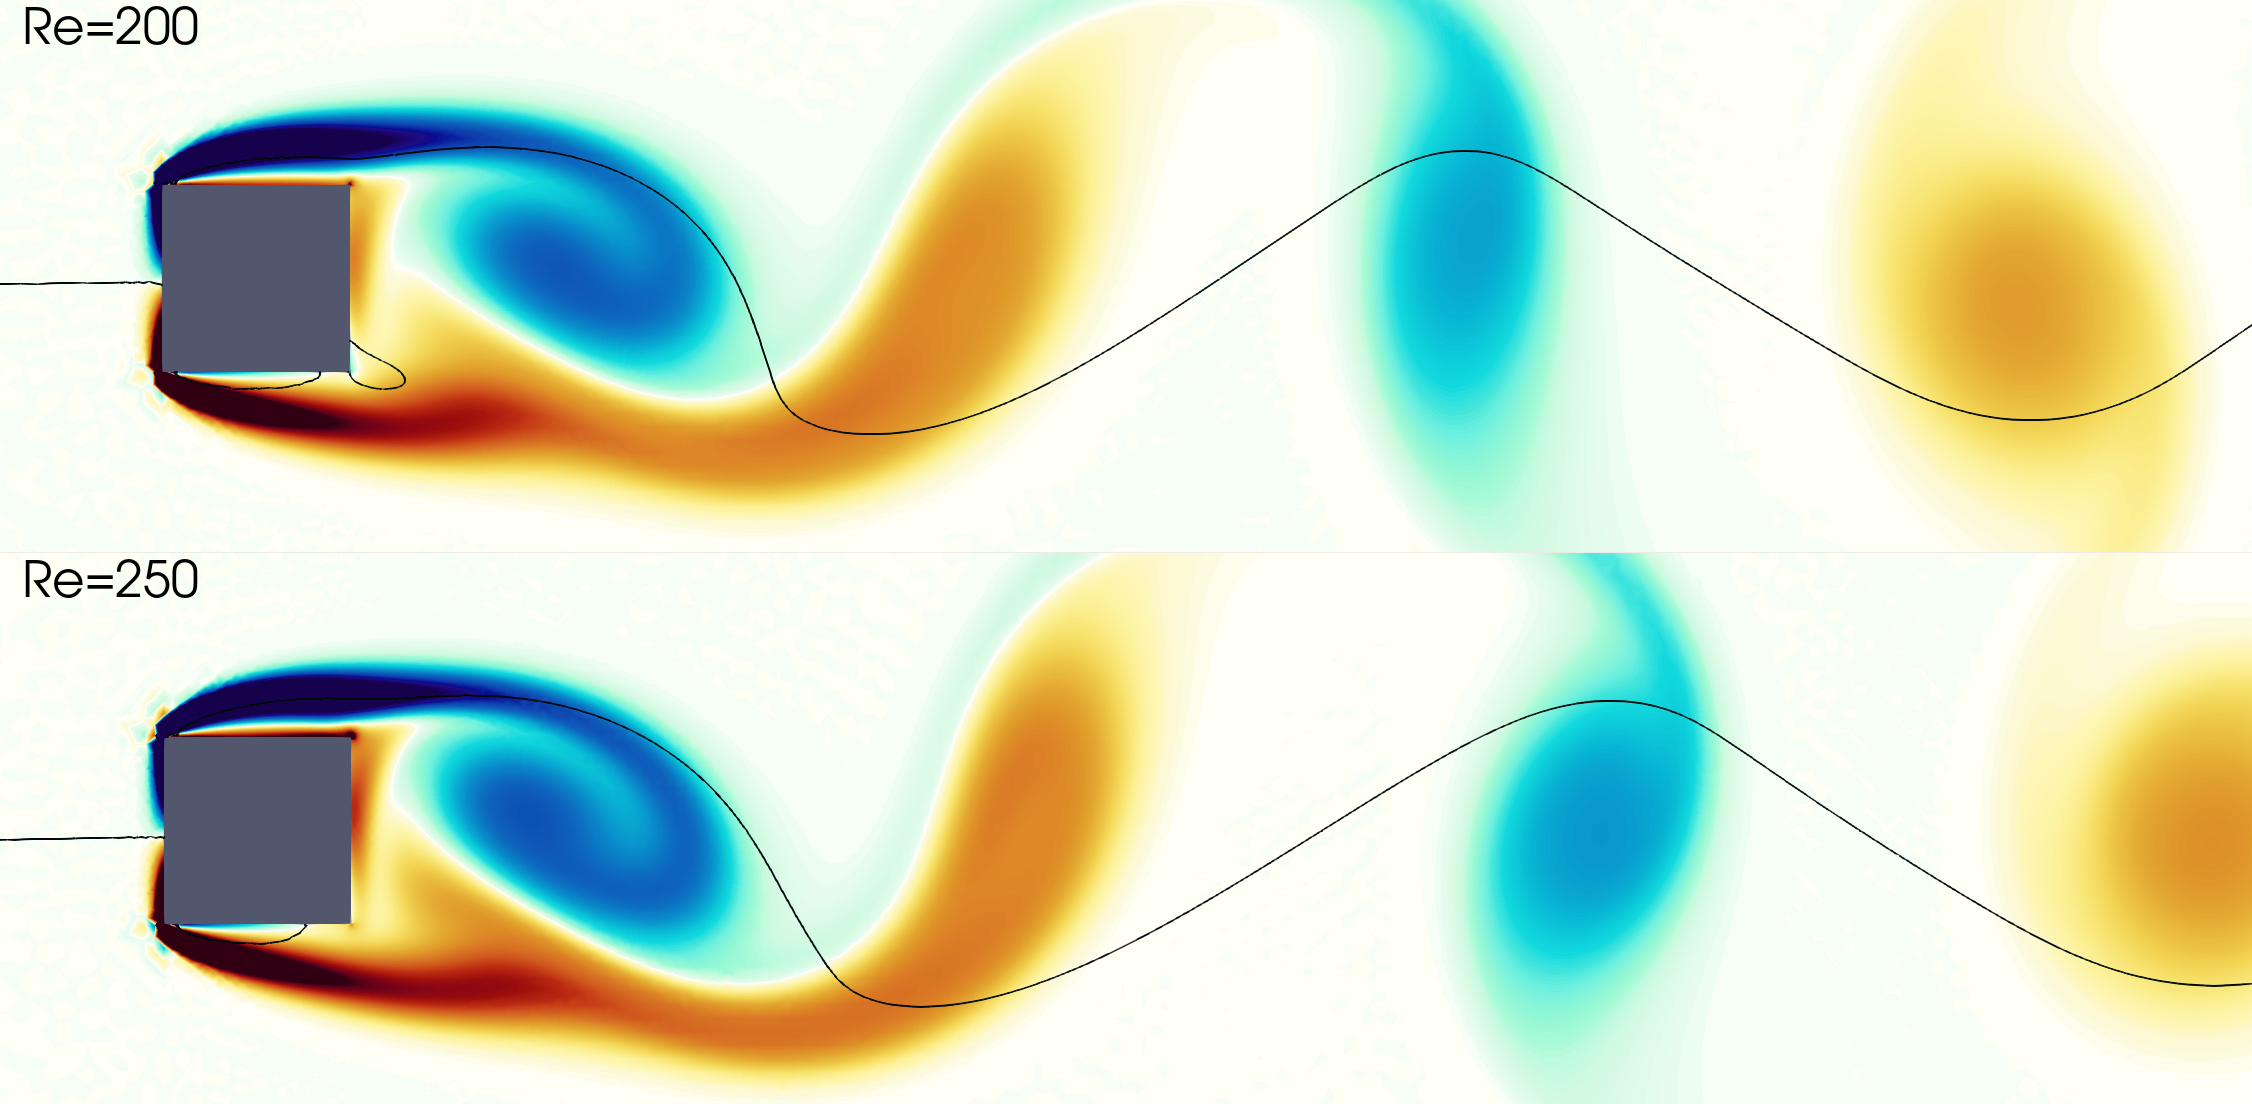
\includegraphics[width=0.49\textwidth]{./fig/AR1/snap/snap.0045.png}  
  \caption{$\AR=1$. Top: $Re=200$. Bottom: $Re=250$. Eight instantaneous snaphots takes equispaced in half of the period.}
\end{figure}      


\begin{figure}
  \centering
  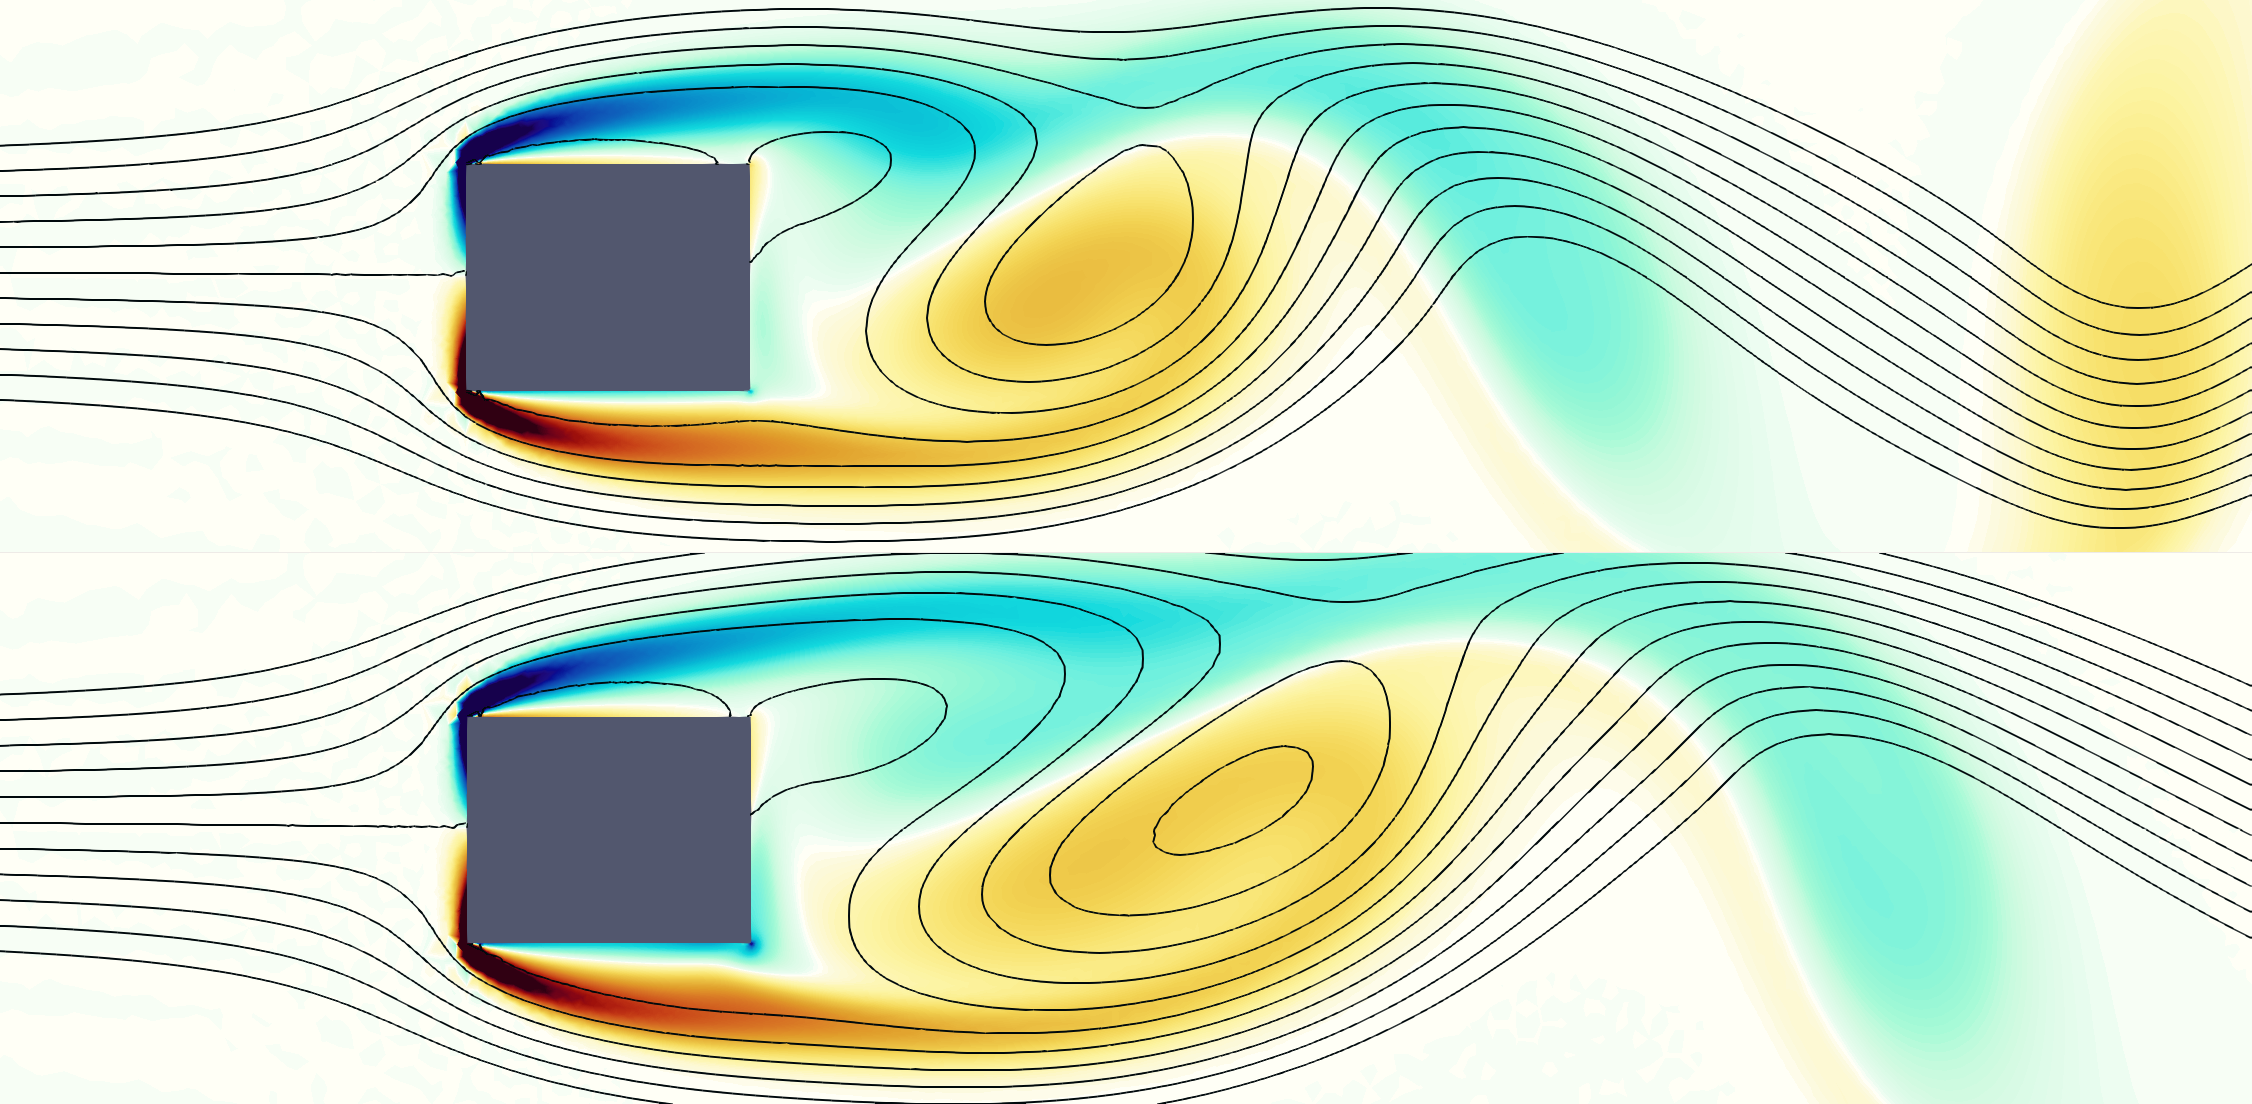
\includegraphics[width=0.49\textwidth]{./fig/AR1p25/snap/snap.0000.png}
  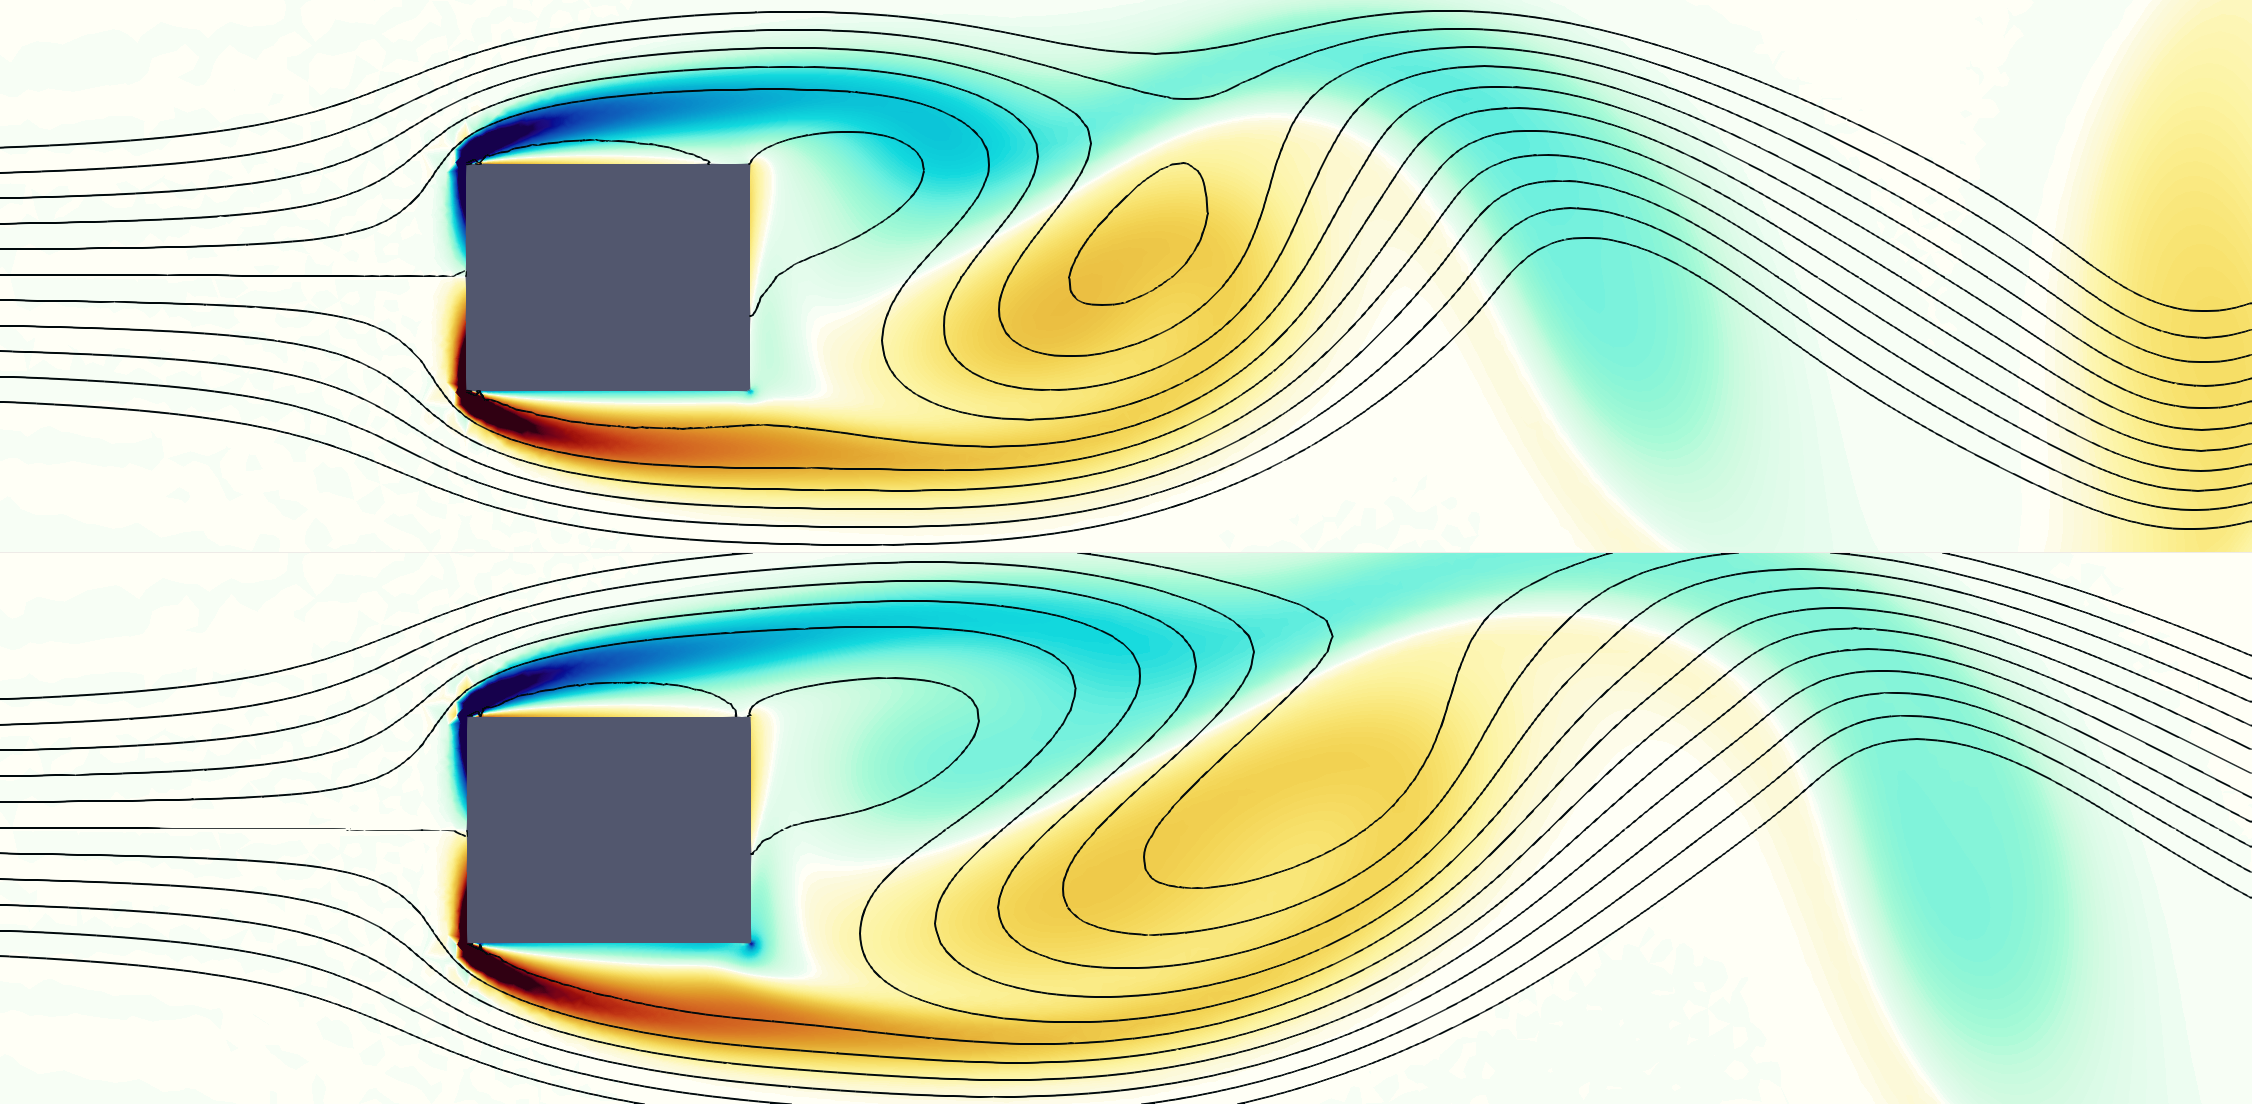
\includegraphics[width=0.49\textwidth]{./fig/AR1p25/snap/snap.0005.png}
  \begin{tikzpicture}
  \draw (-10,2) -- (8,2);
  \end{tikzpicture}
  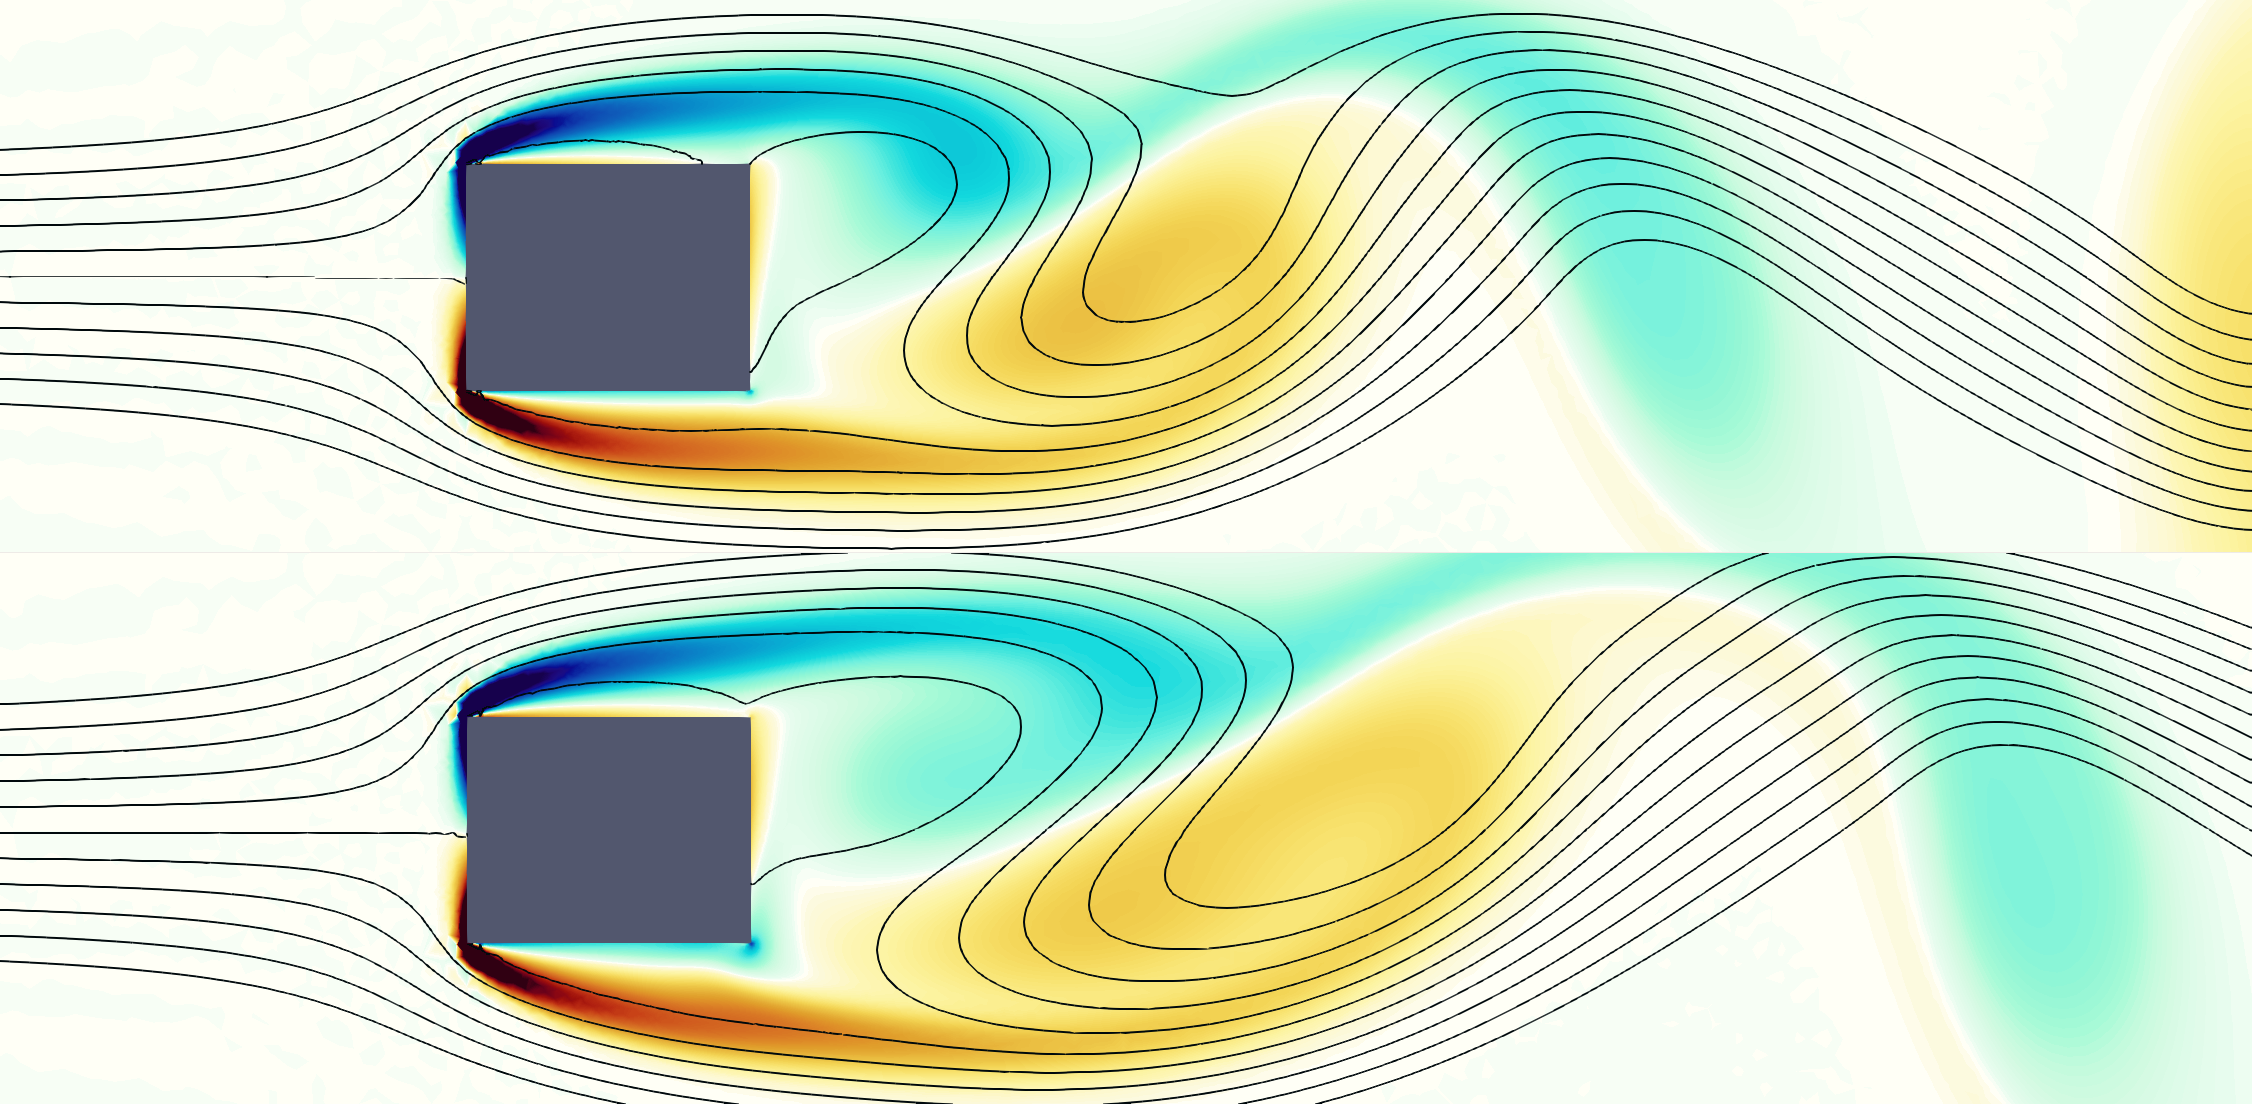
\includegraphics[width=0.49\textwidth]{./fig/AR1p25/snap/snap.0010.png}
  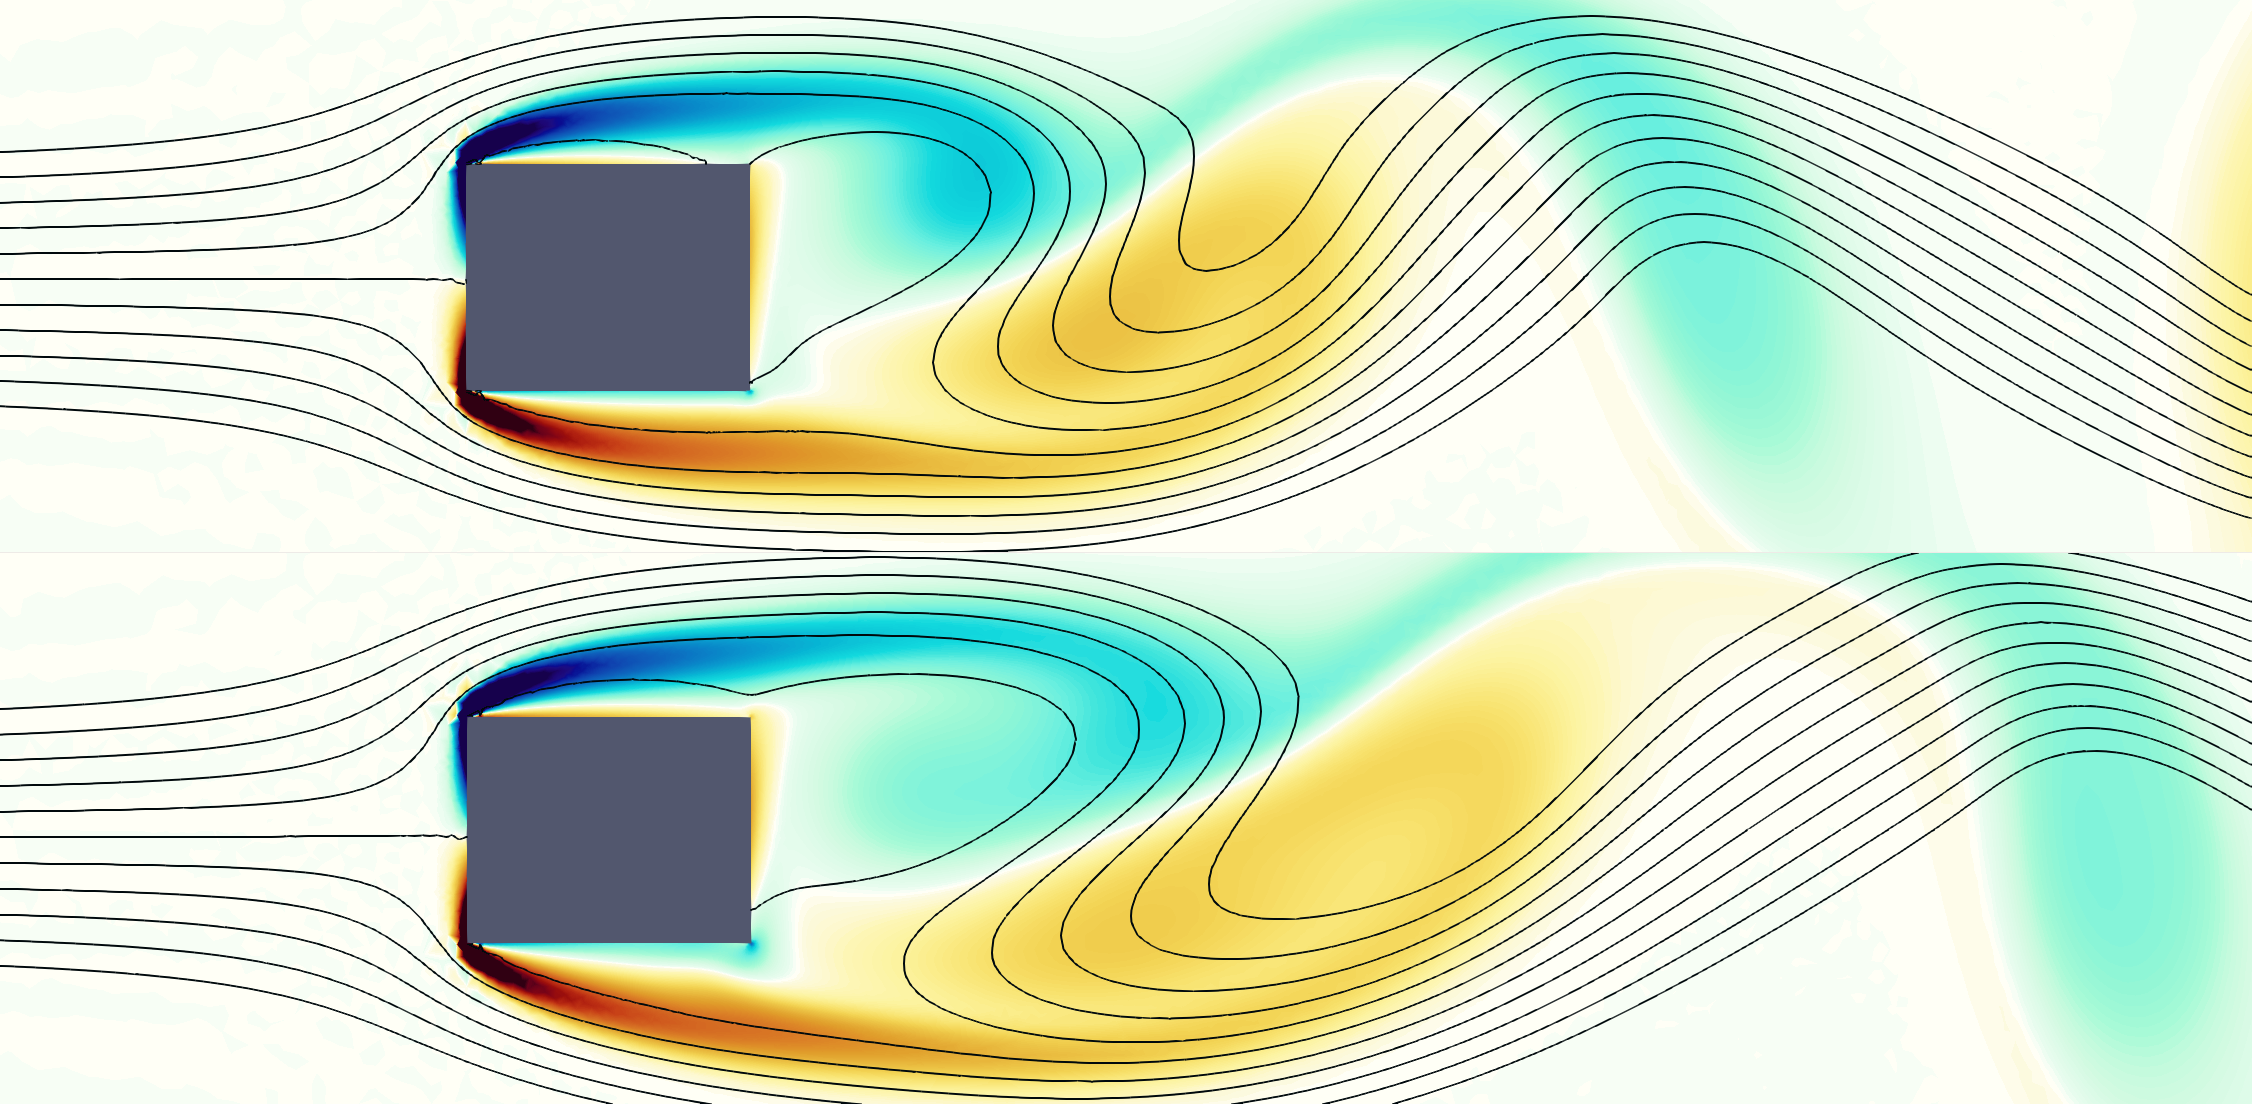
\includegraphics[width=0.49\textwidth]{./fig/AR1p25/snap/snap.0015.png}
  \begin{tikzpicture}
  \draw (-10,2) -- (8,2);
  \end{tikzpicture}
  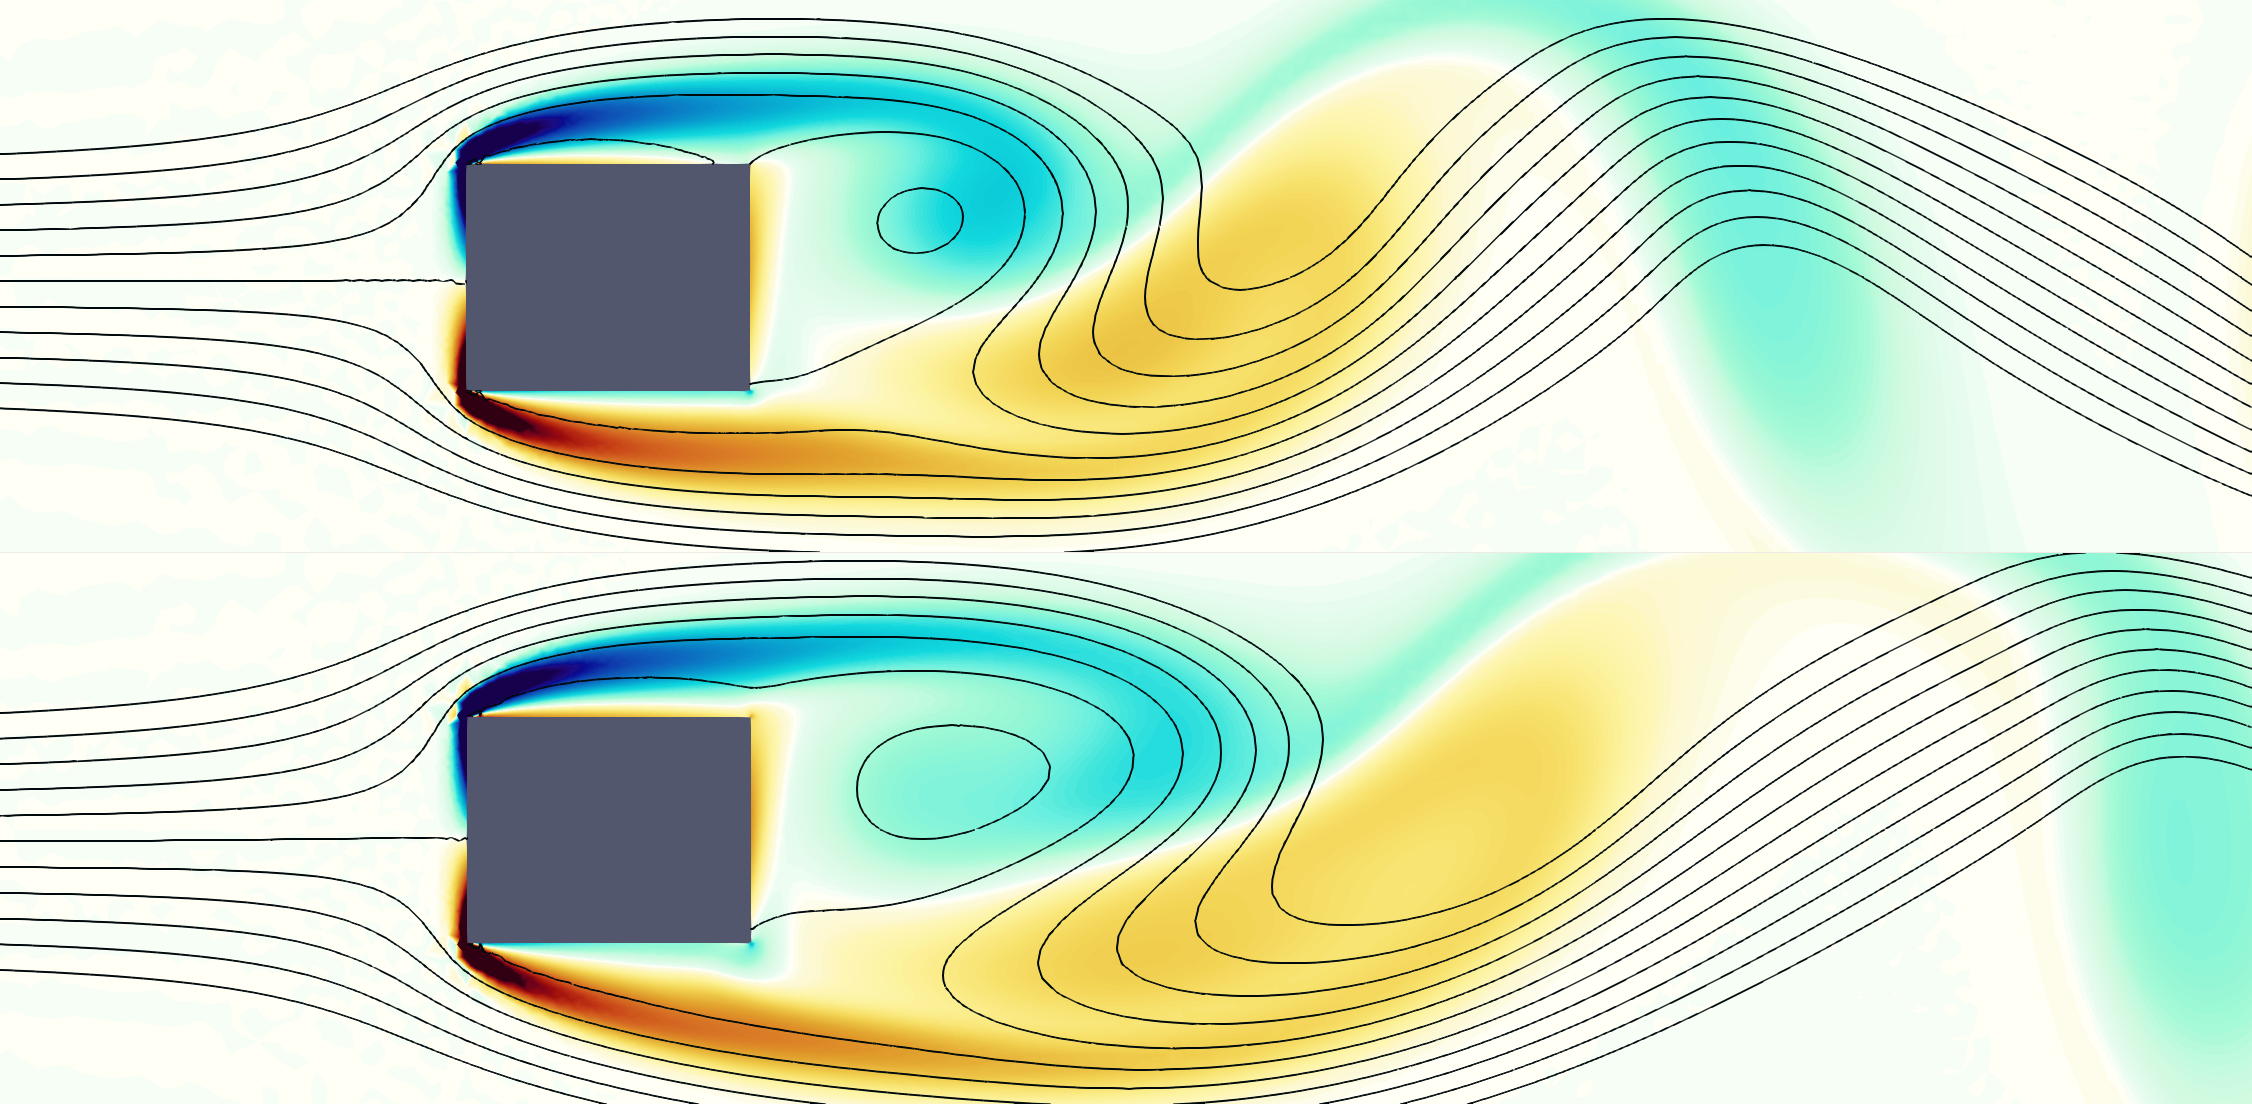
\includegraphics[width=0.49\textwidth]{./fig/AR1p25/snap/snap.0020.png}
  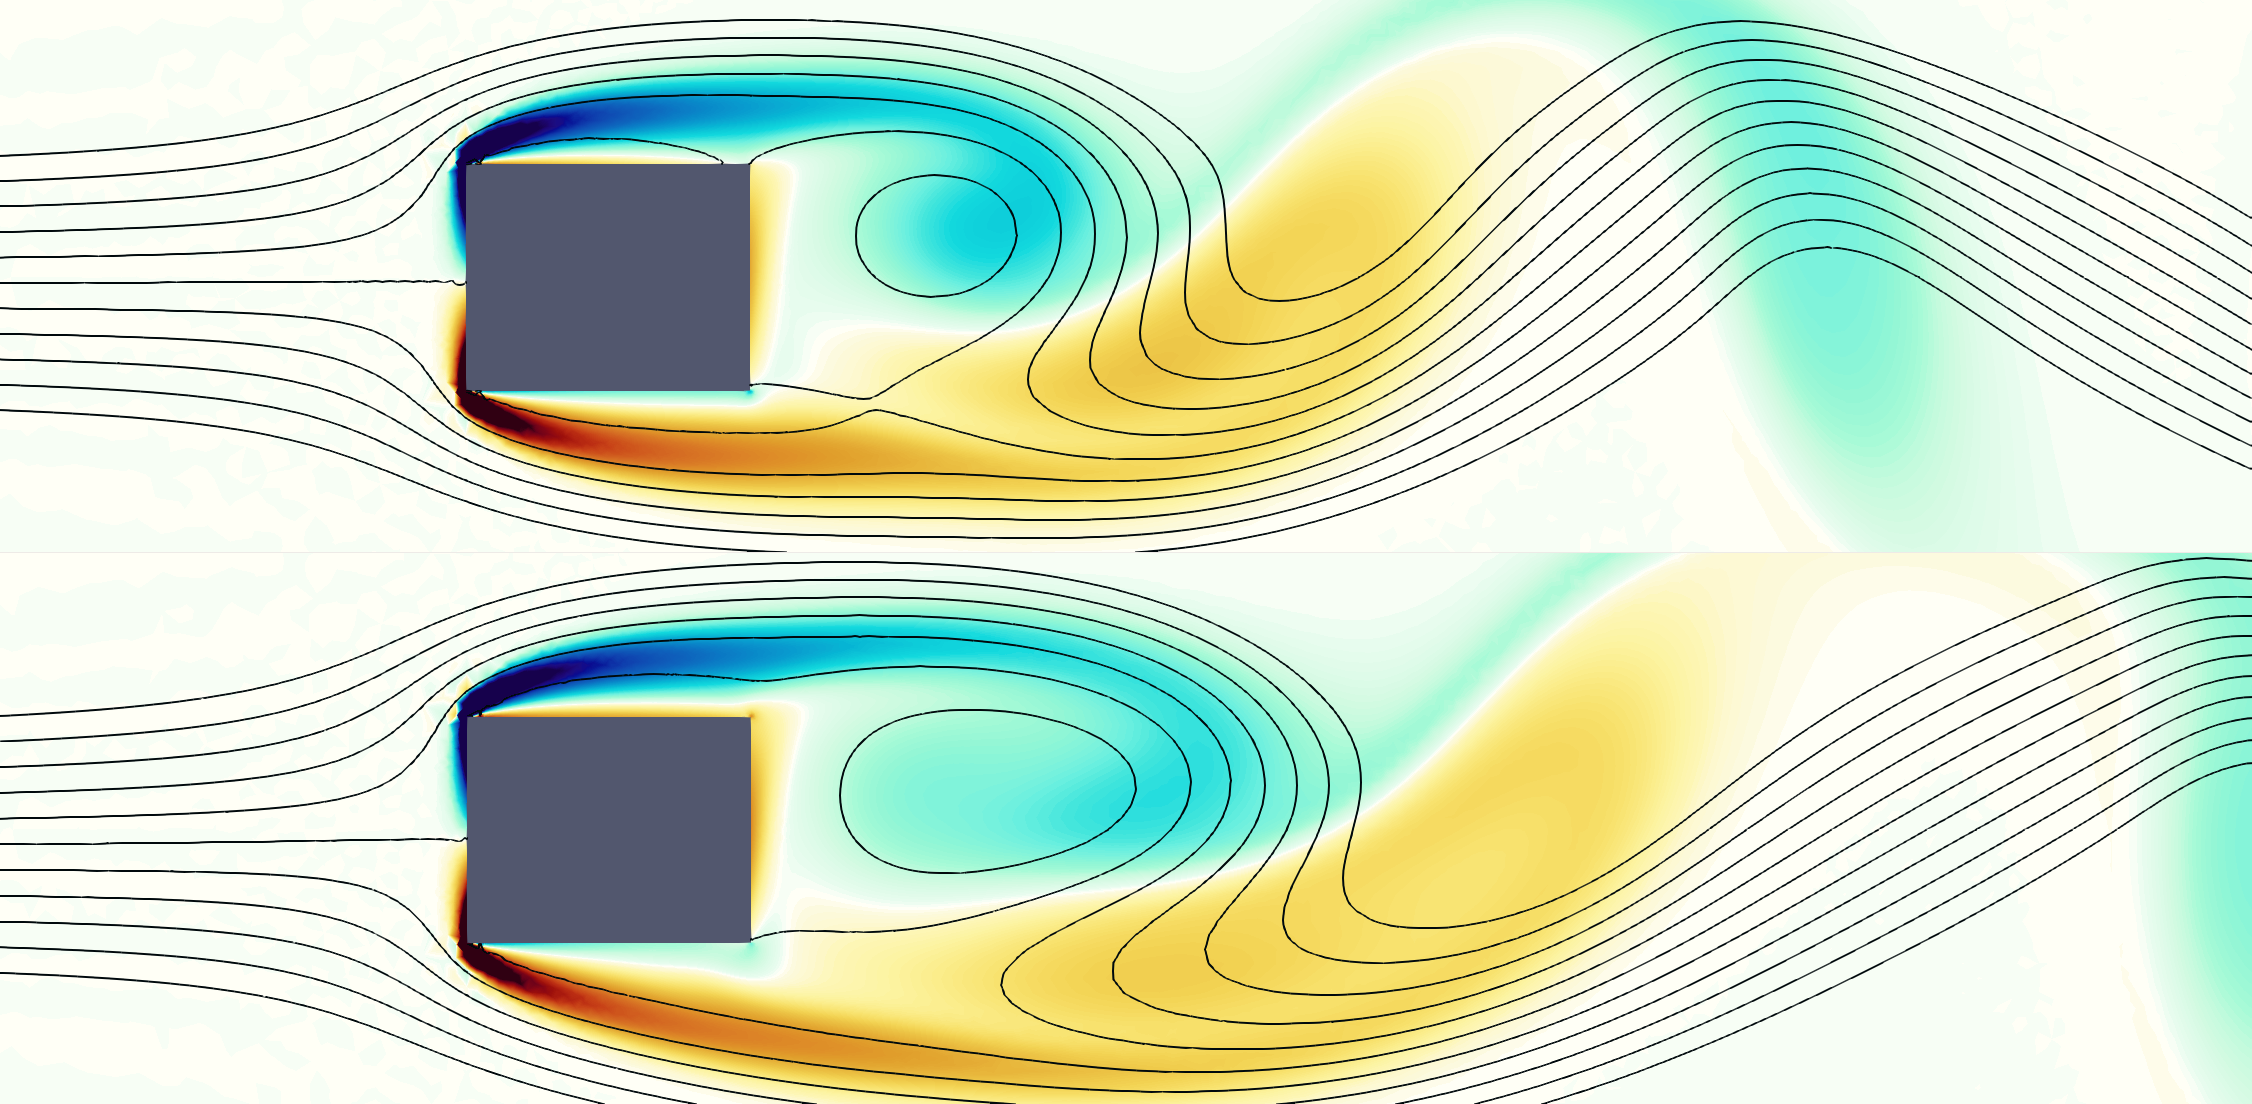
\includegraphics[width=0.49\textwidth]{./fig/AR1p25/snap/snap.0025.png}
  \begin{tikzpicture}
  \draw (-10,2) -- (8,2);
  \end{tikzpicture}
  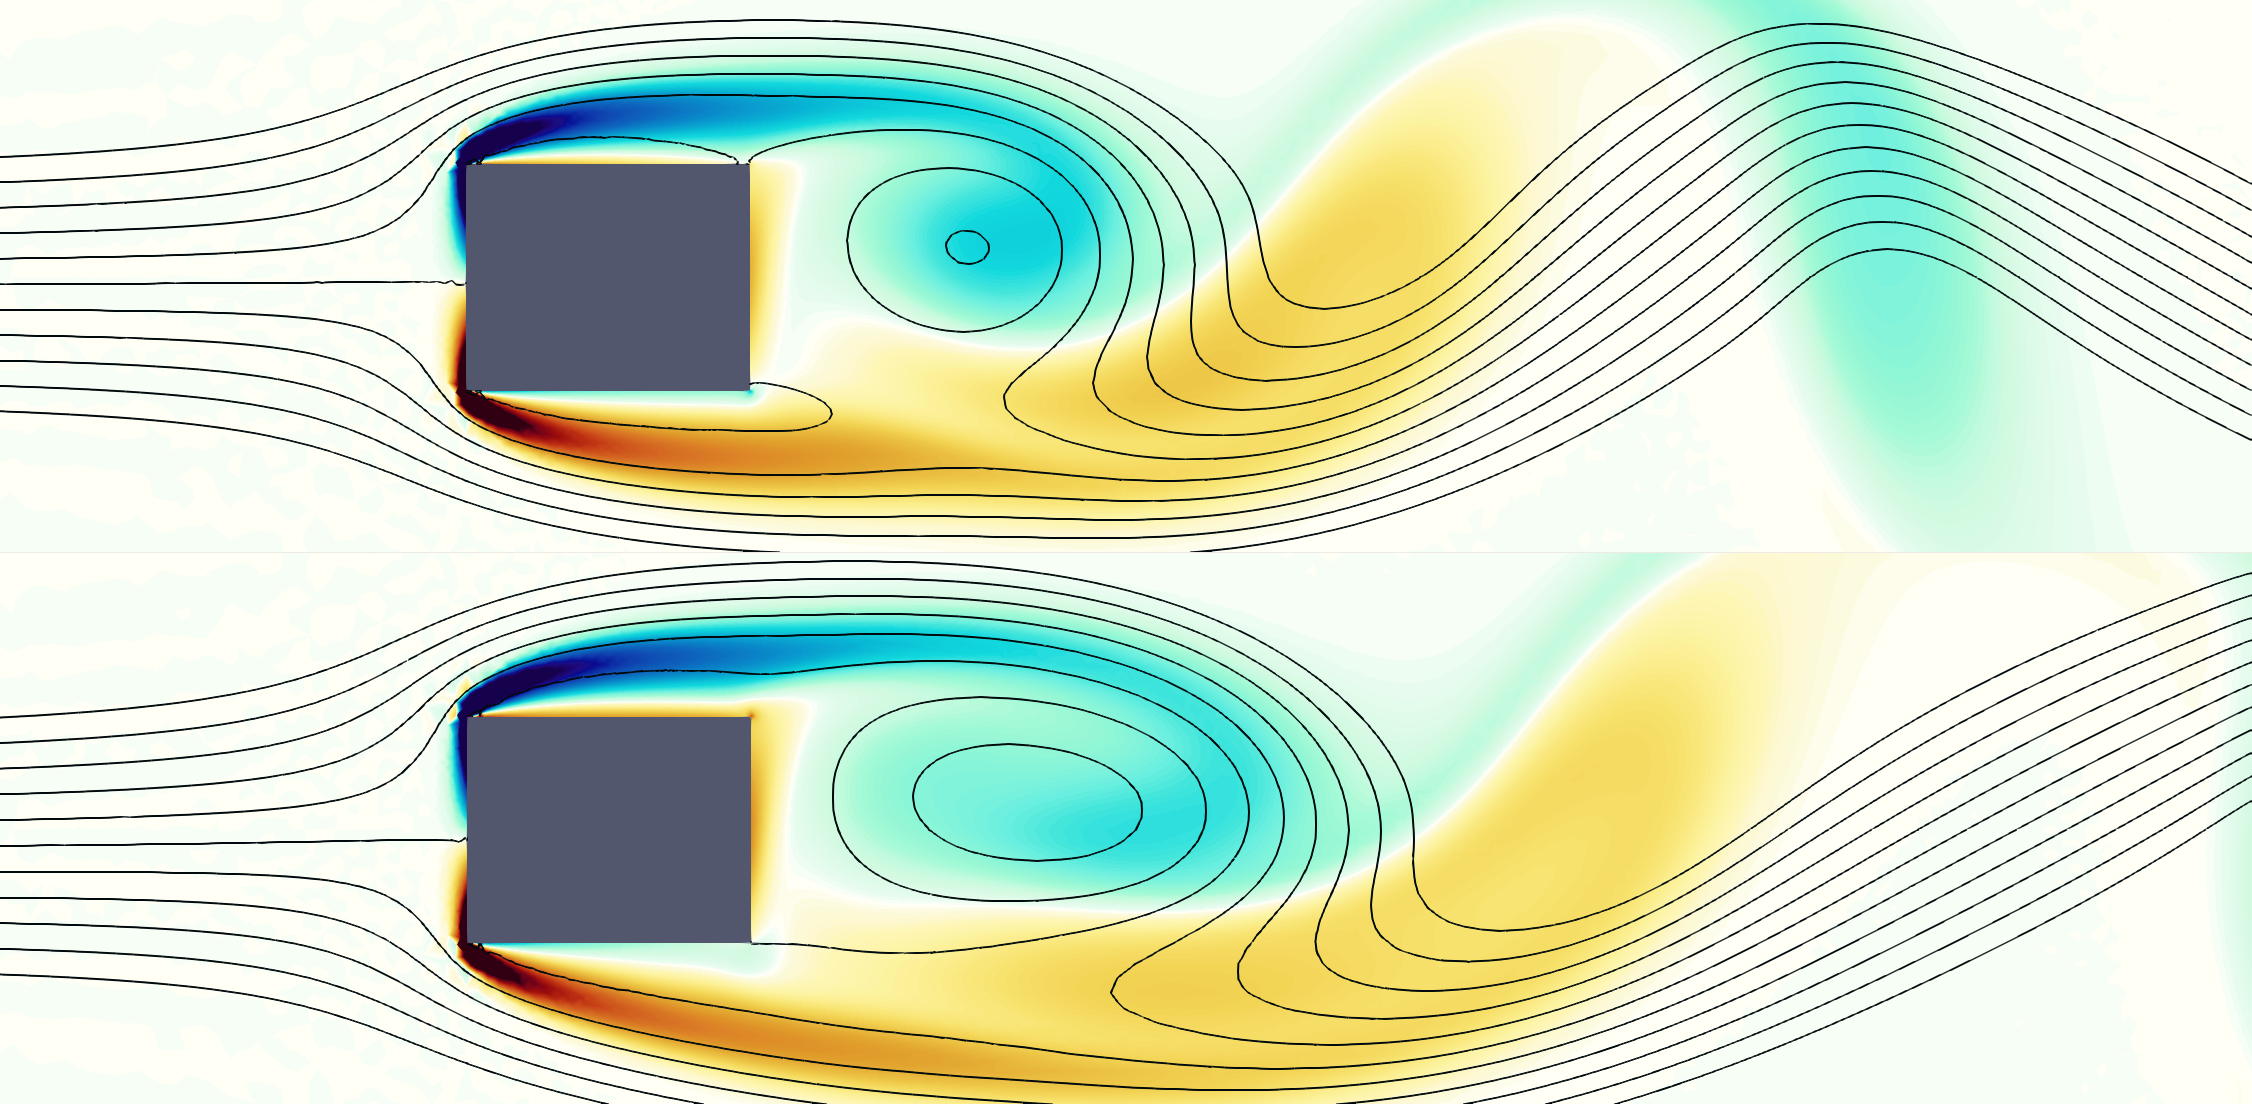
\includegraphics[width=0.49\textwidth]{./fig/AR1p25/snap/snap.0030.png}
  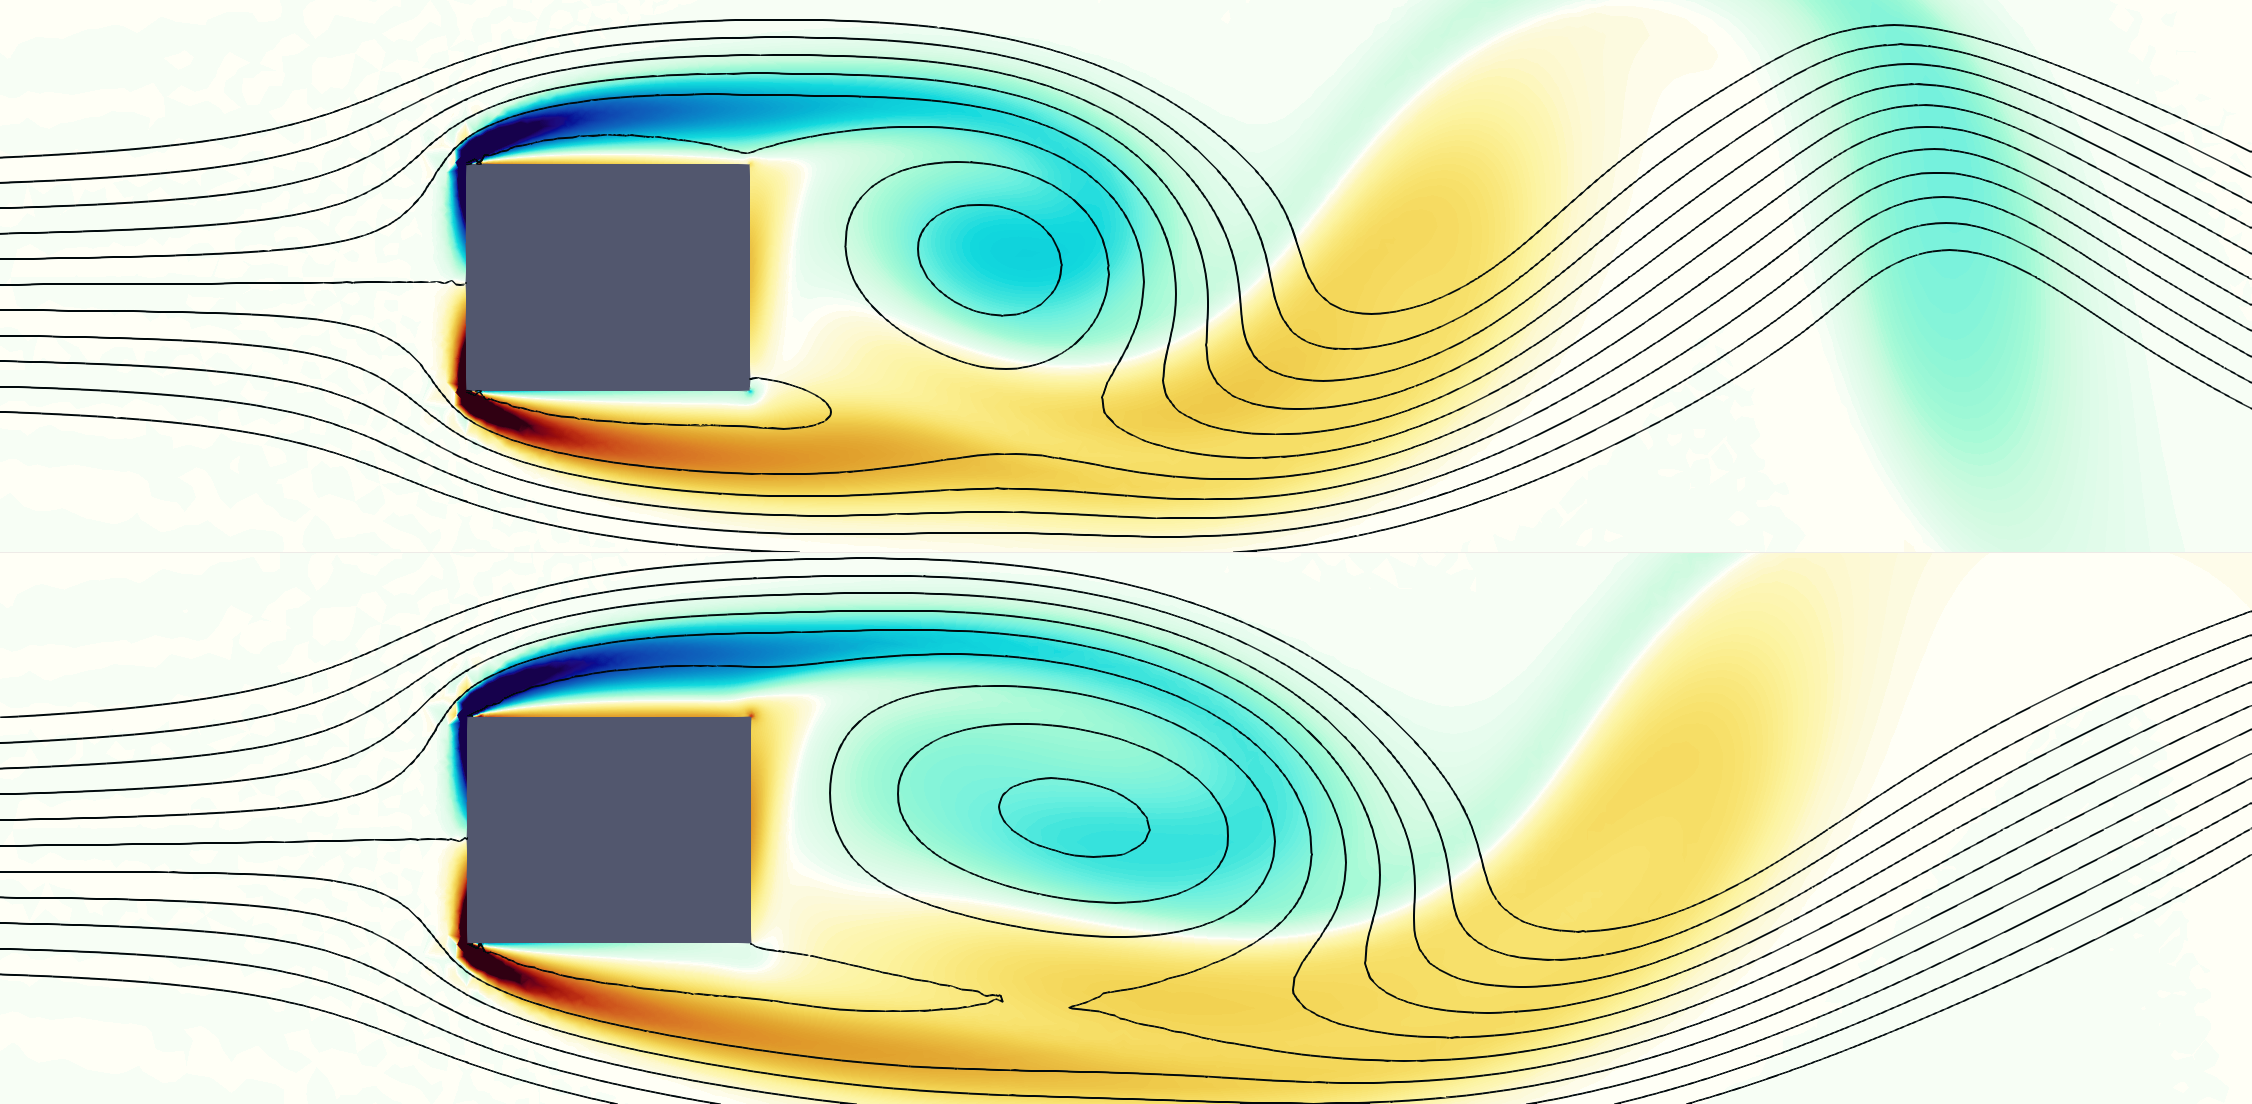
\includegraphics[width=0.49\textwidth]{./fig/AR1p25/snap/snap.0035.png}
  \begin{tikzpicture}
  \draw (-10,2) -- (8,2);
  \end{tikzpicture}
  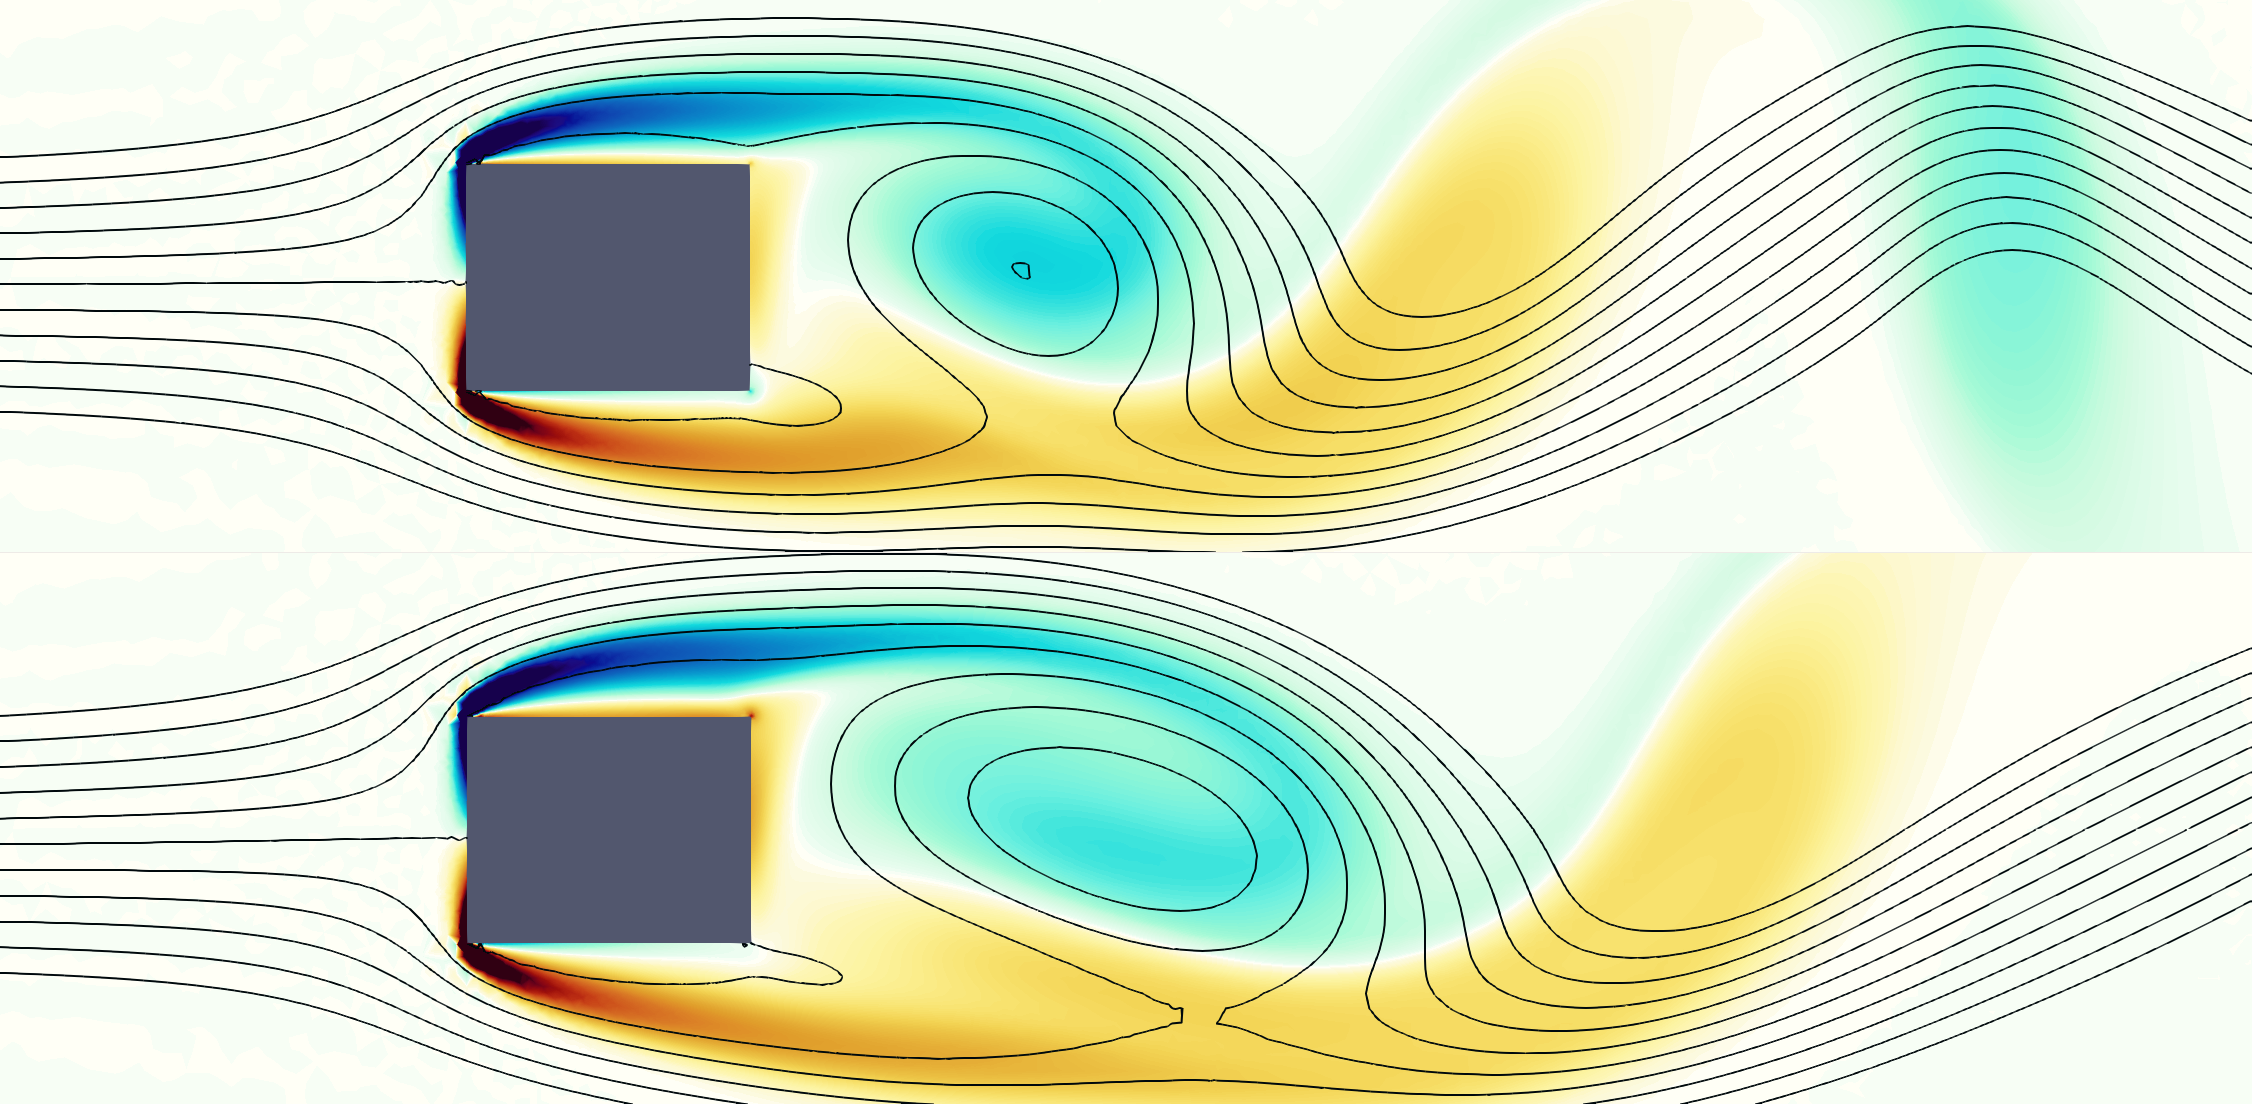
\includegraphics[width=0.49\textwidth]{./fig/AR1p25/snap/snap.0040.png}
  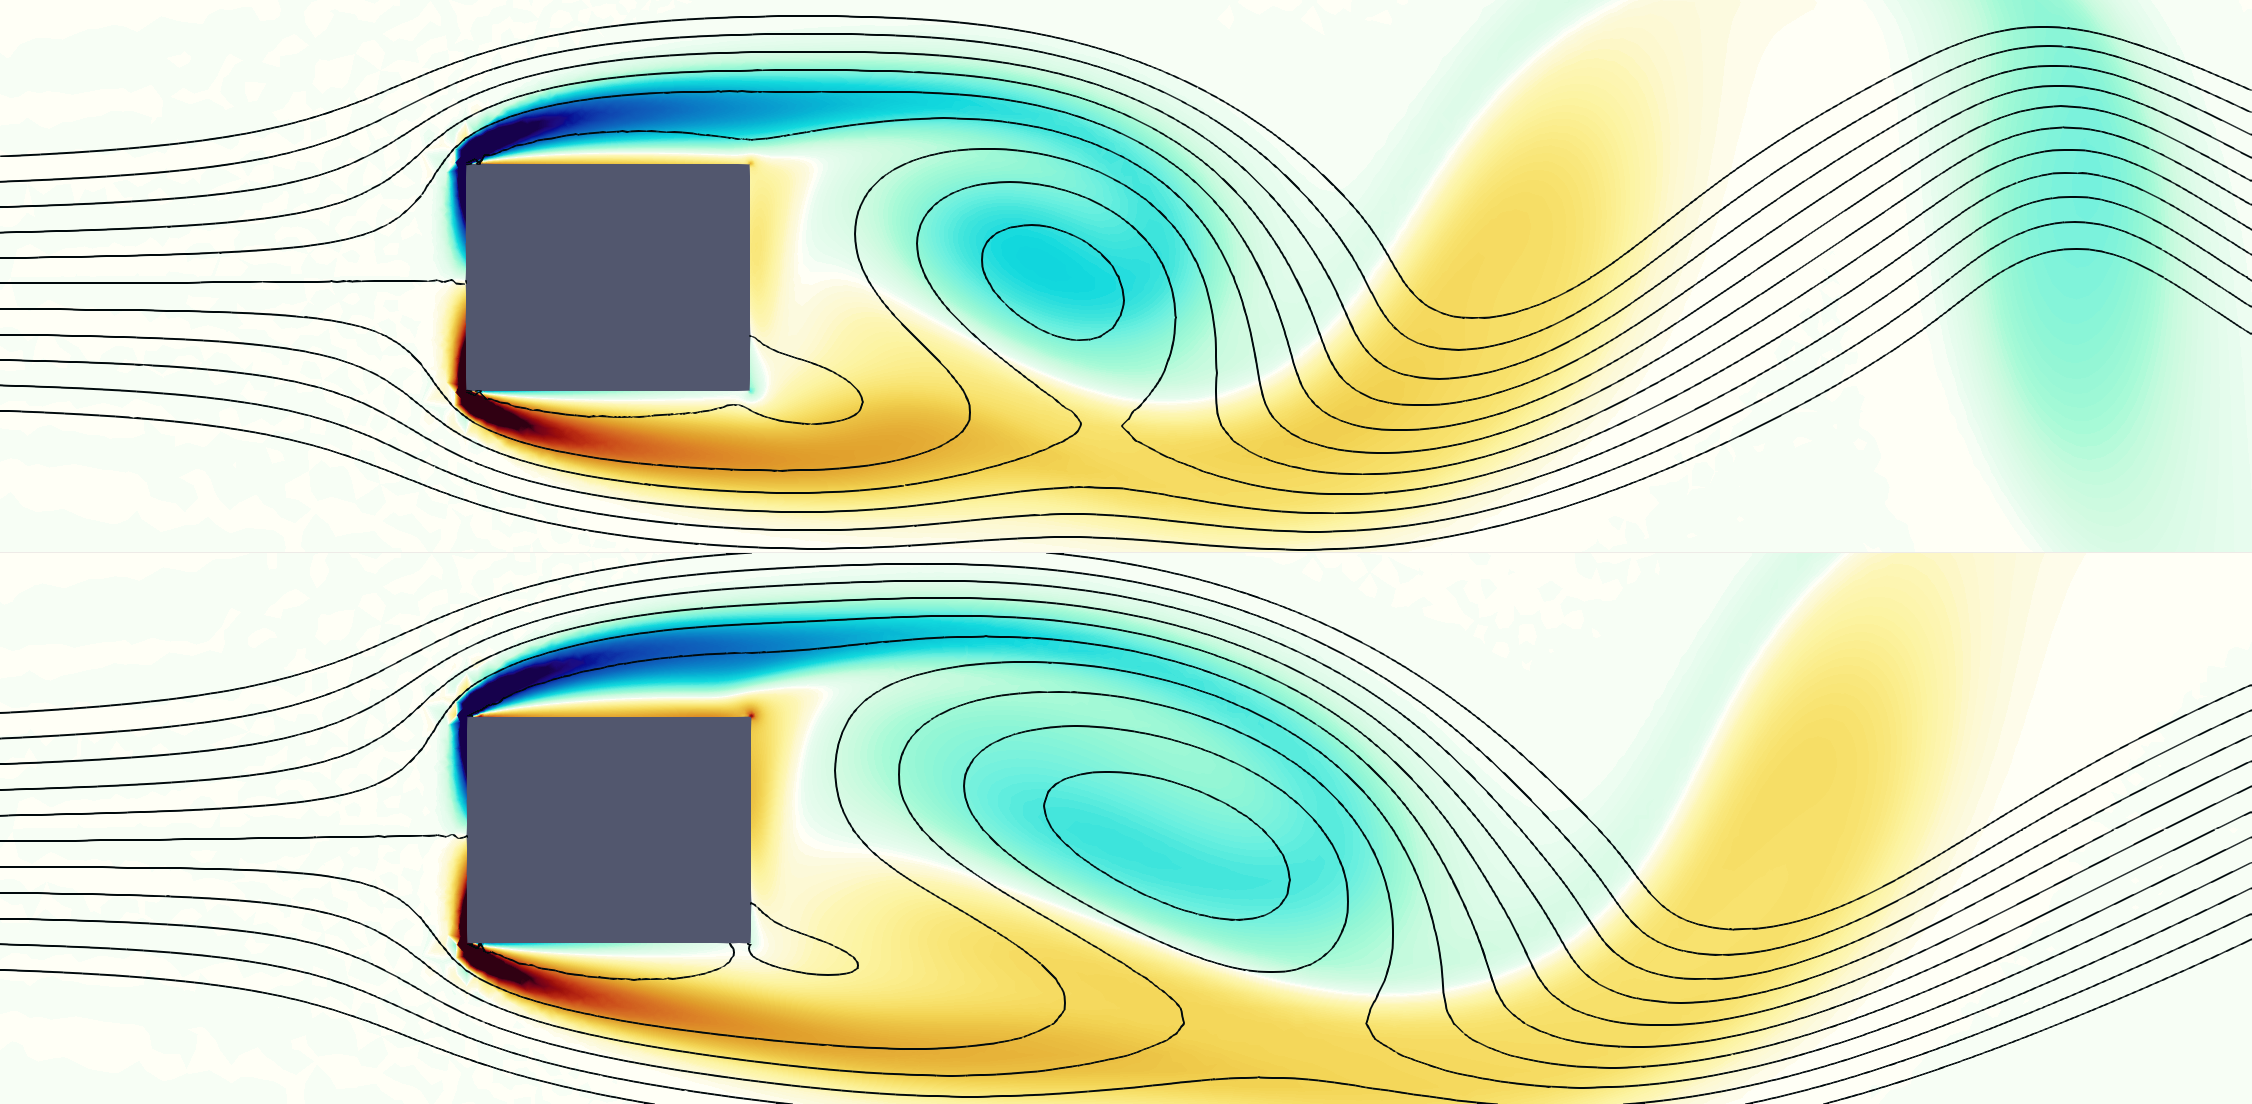
\includegraphics[width=0.49\textwidth]{./fig/AR1p25/snap/snap.0045.png}  
  \caption{$\AR=1.25$. Top: $Re=200$. Bottom: $Re=250$. Eight instantaneous snaphots takes equispaced in half of the period.}
\end{figure}      

\begin{figure}
  \centering
  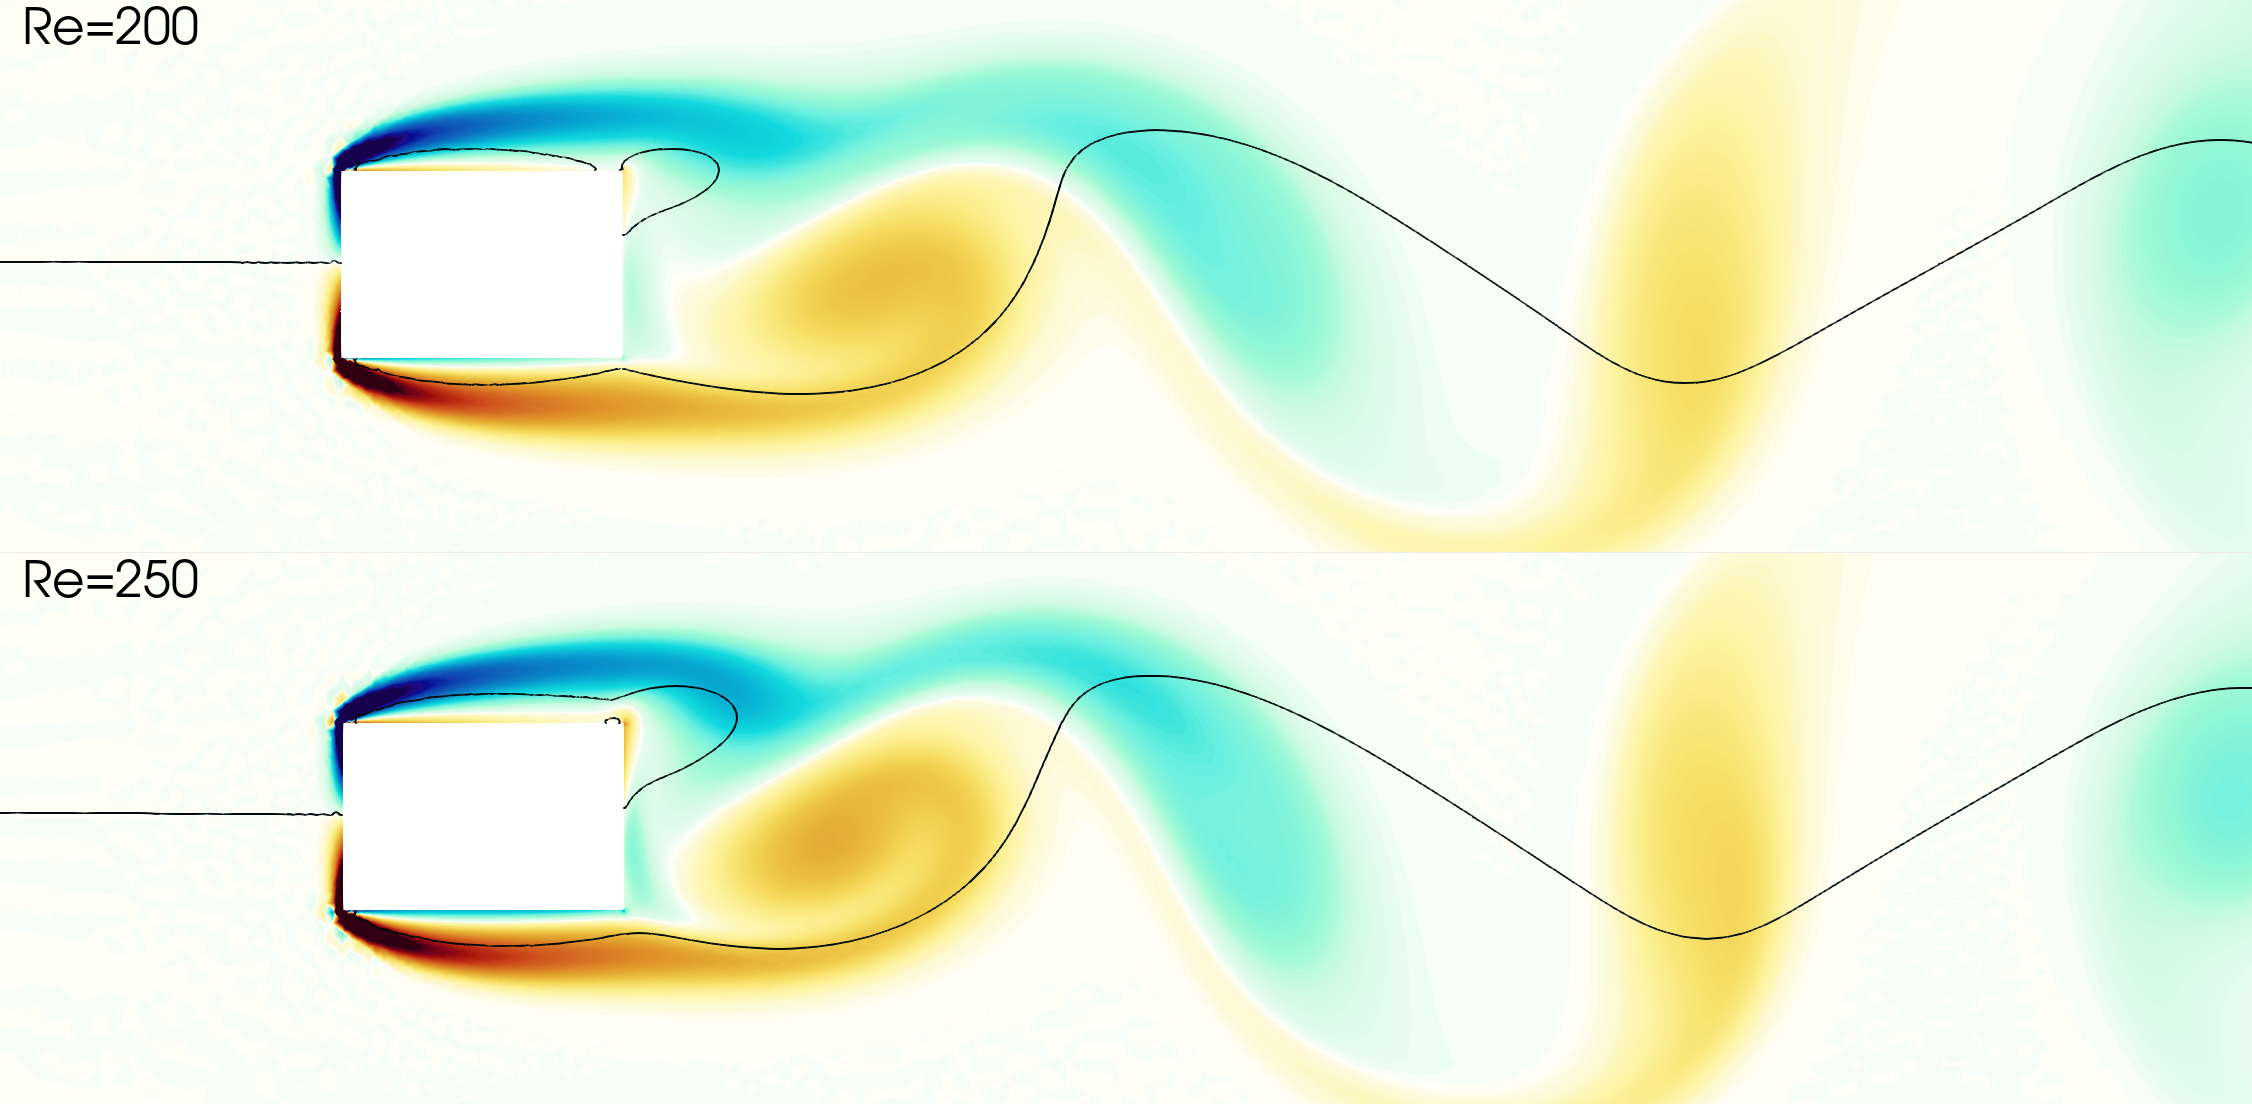
\includegraphics[width=0.49\textwidth]{./fig/AR1p5/snap/snap.0000.png}
  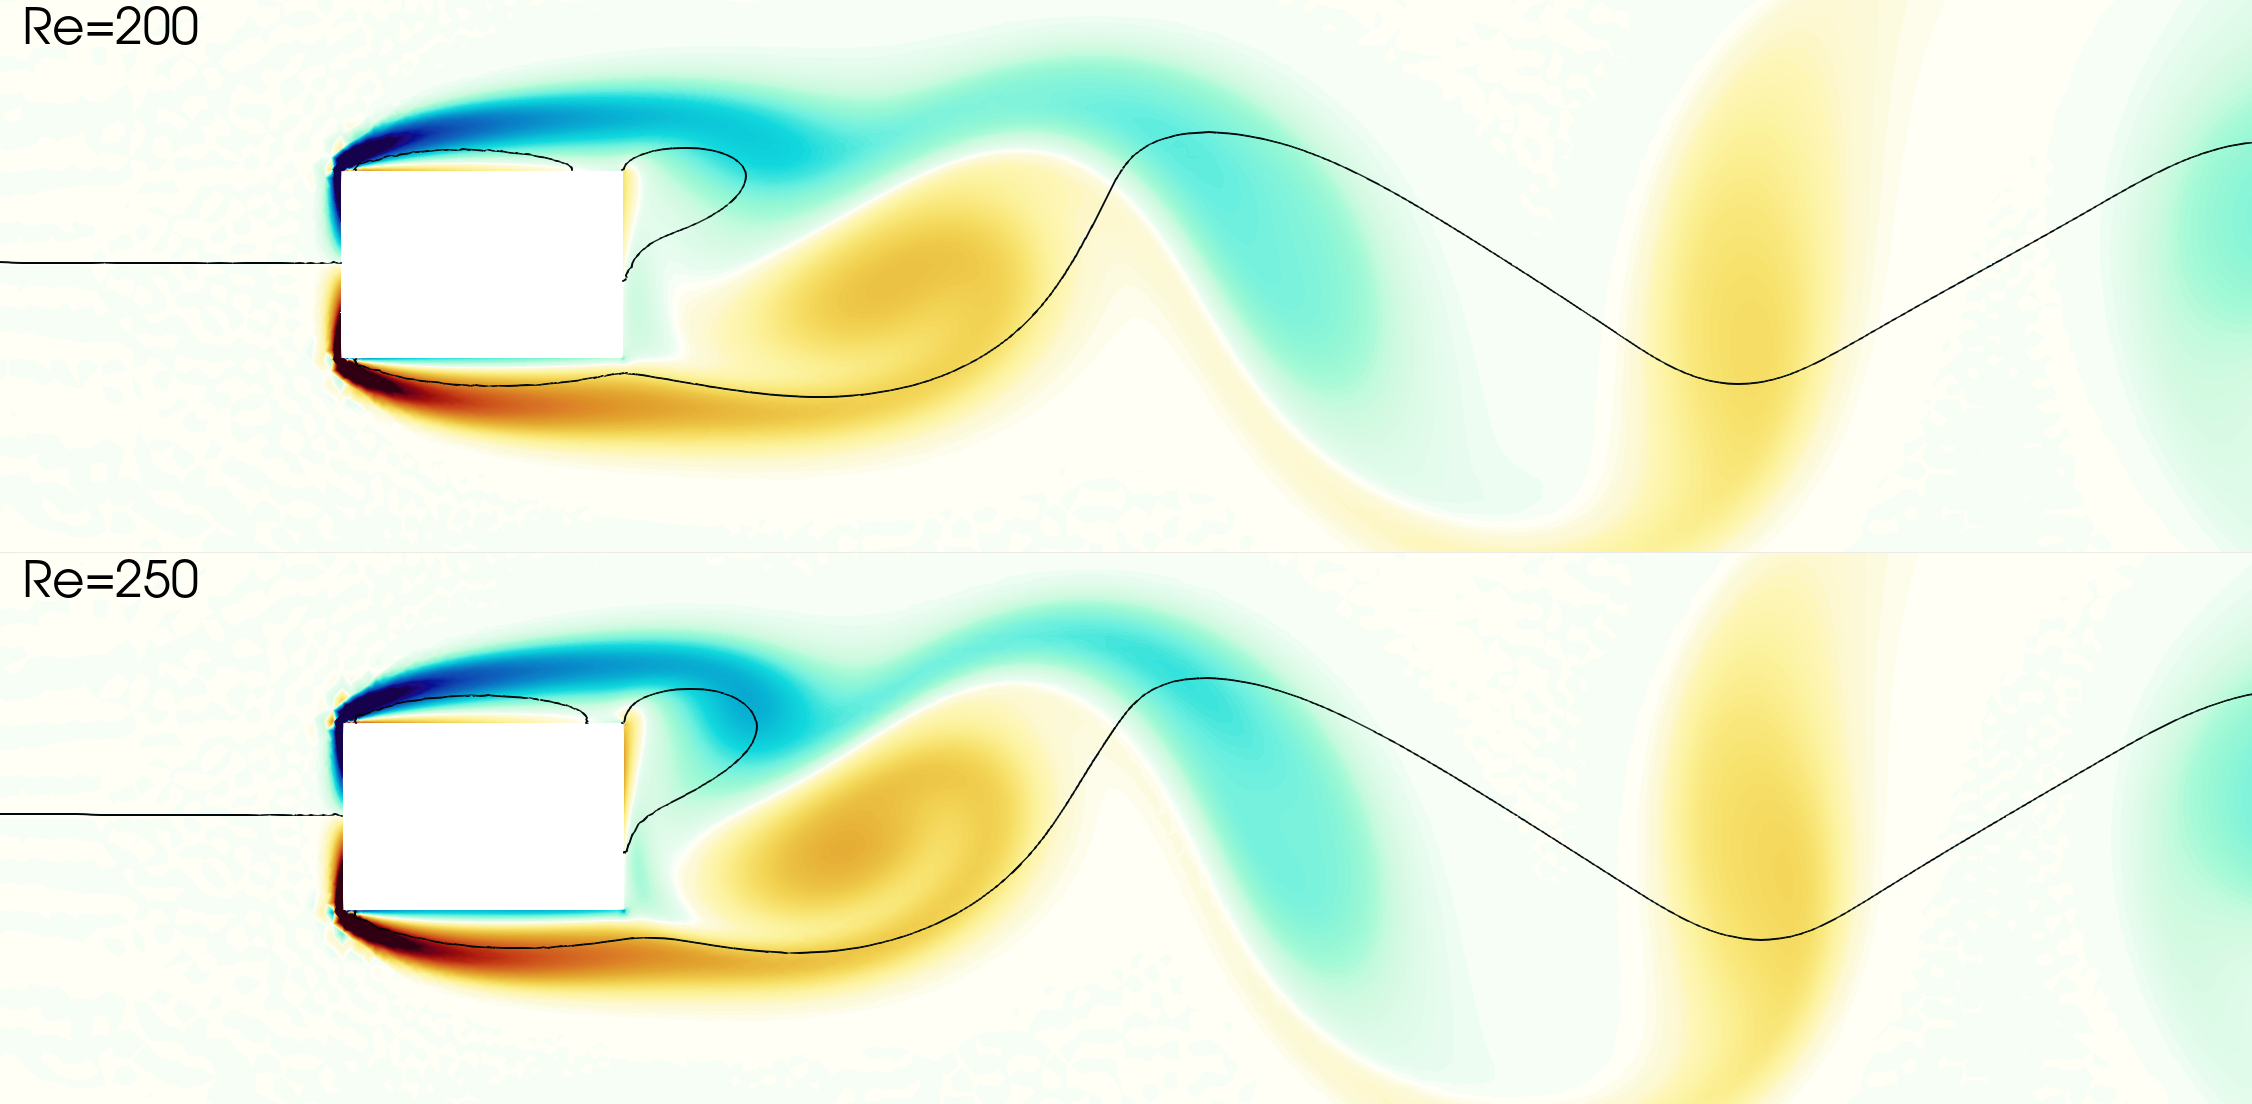
\includegraphics[width=0.49\textwidth]{./fig/AR1p5/snap/snap.0005.png}
  \begin{tikzpicture}
  \draw (-10,2) -- (8,2);
  \end{tikzpicture}
  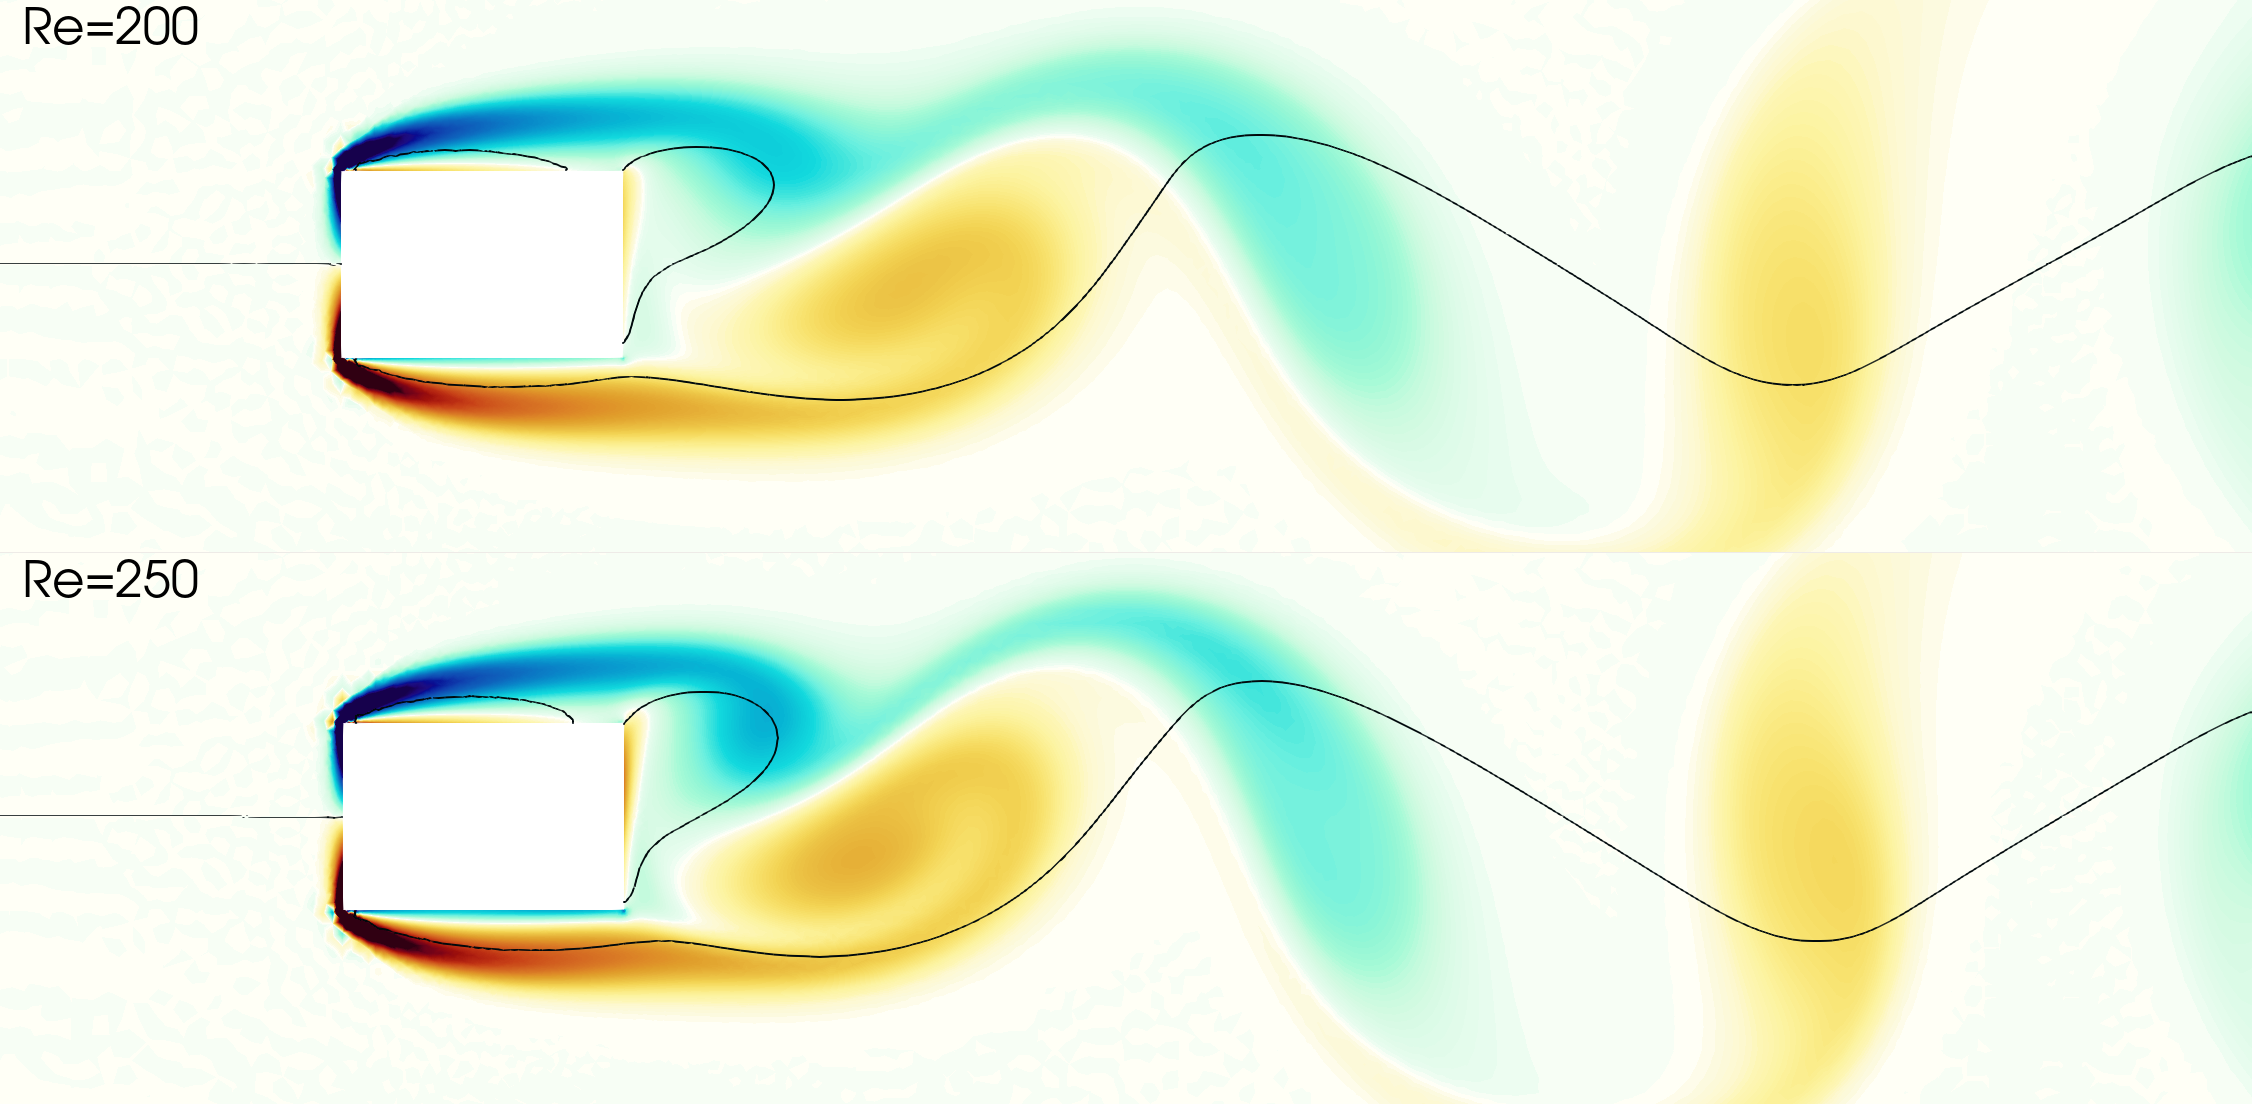
\includegraphics[width=0.49\textwidth]{./fig/AR1p5/snap/snap.0010.png}
  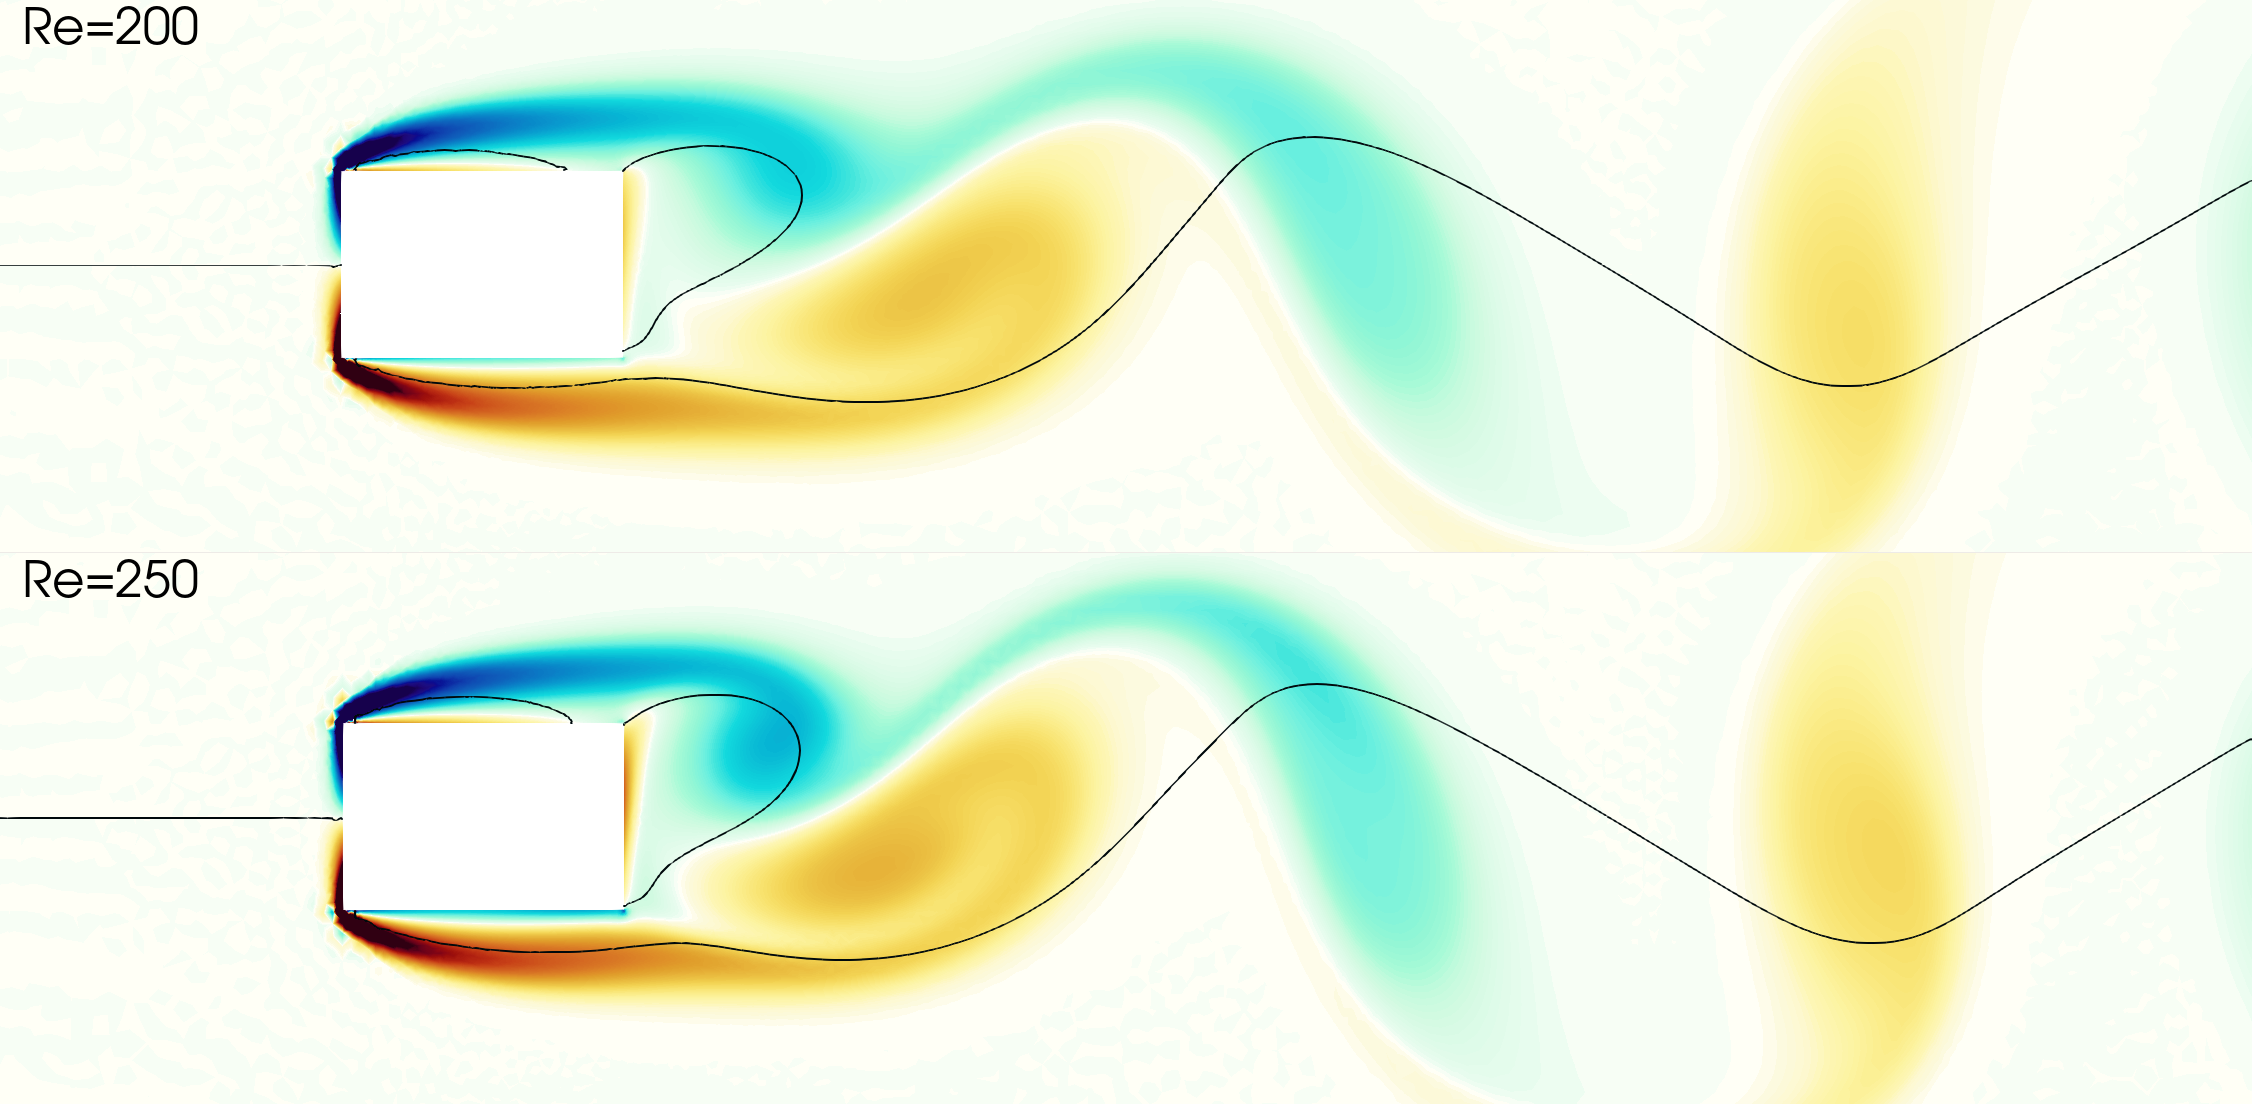
\includegraphics[width=0.49\textwidth]{./fig/AR1p5/snap/snap.0015.png}
  \begin{tikzpicture}
  \draw (-10,2) -- (8,2);
  \end{tikzpicture}
  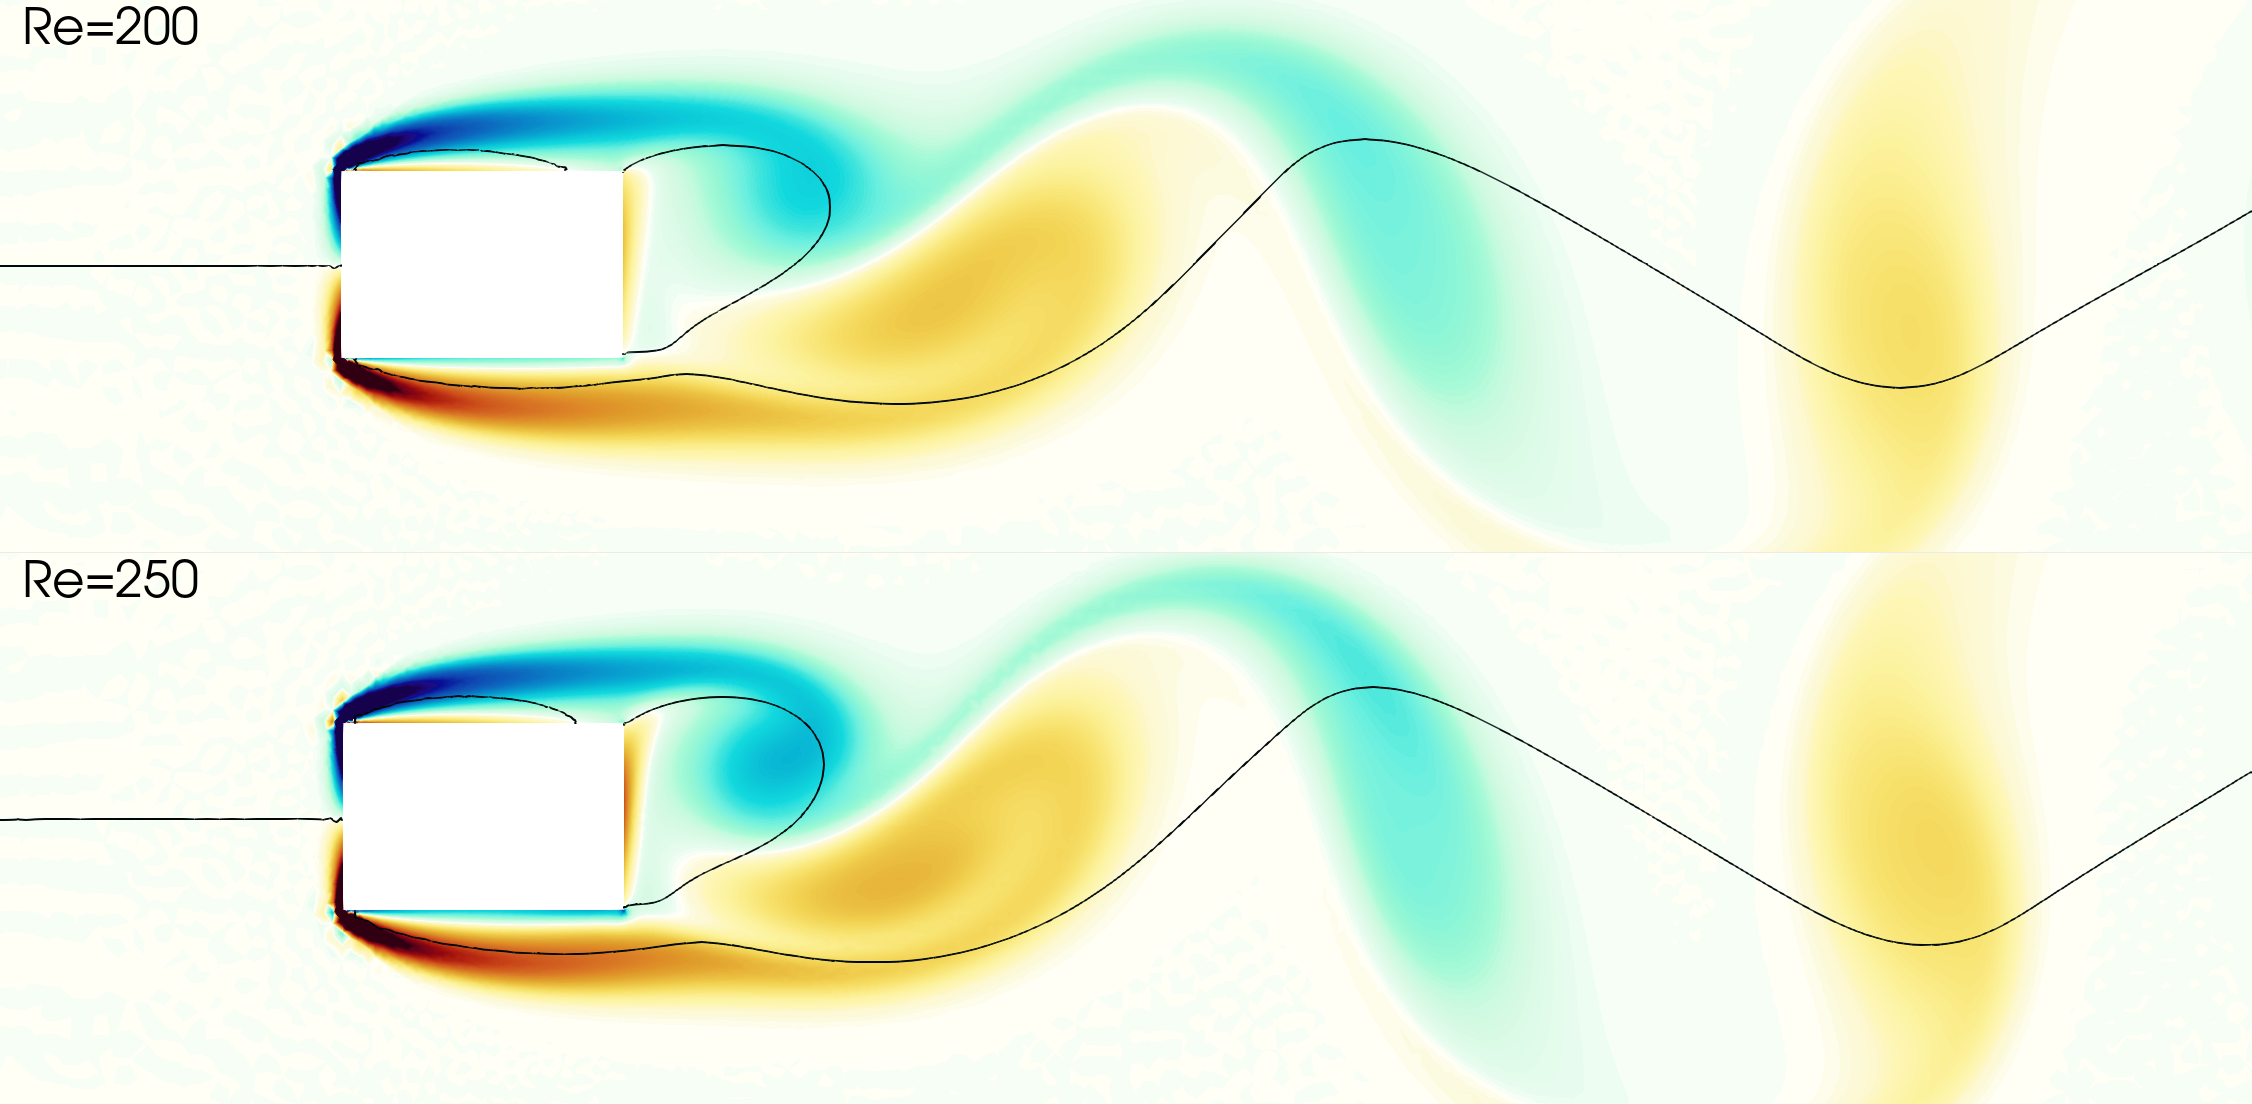
\includegraphics[width=0.49\textwidth]{./fig/AR1p5/snap/snap.0020.png}
  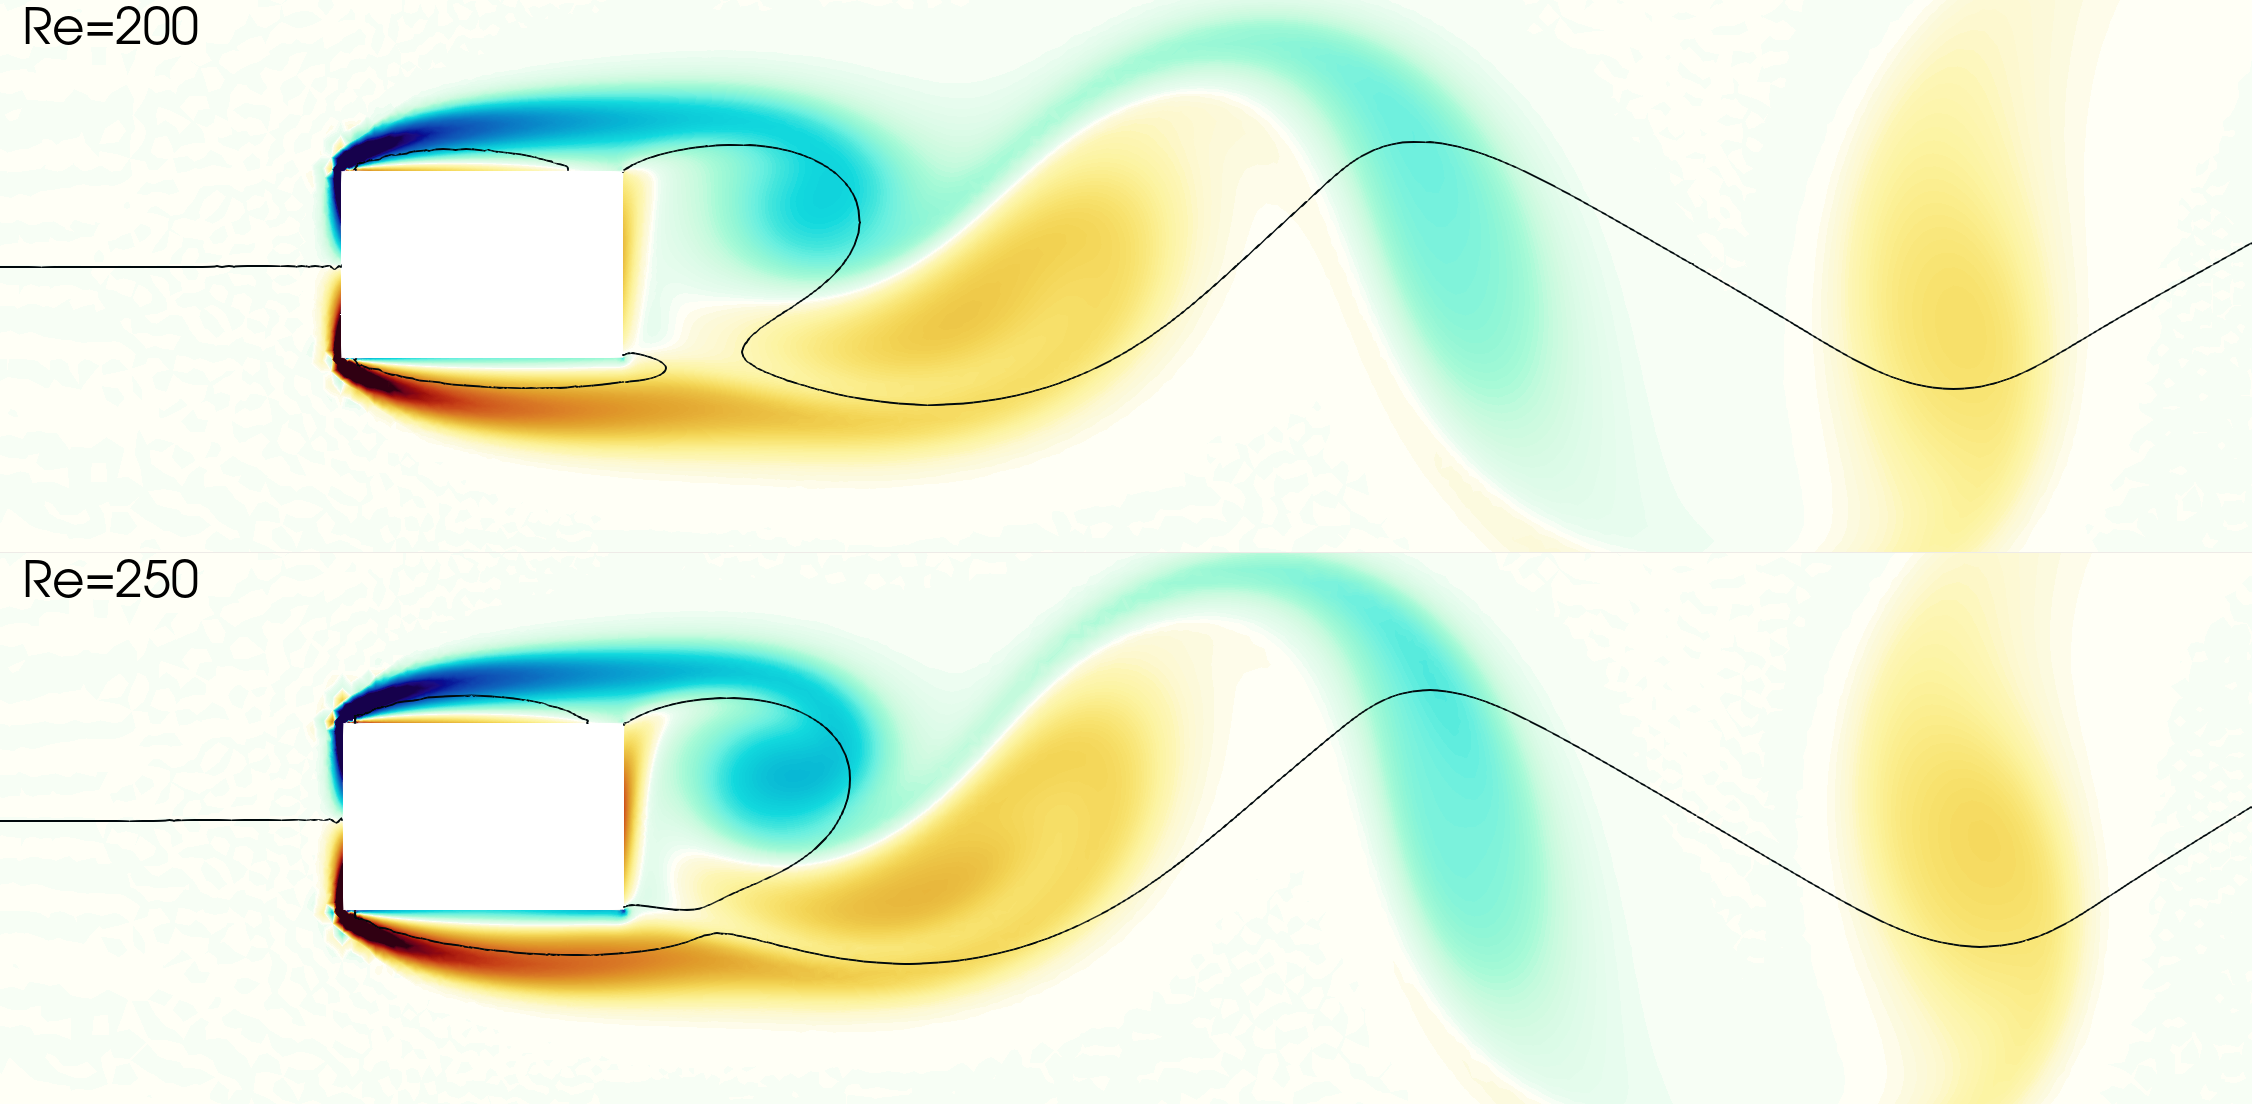
\includegraphics[width=0.49\textwidth]{./fig/AR1p5/snap/snap.0025.png}
  \begin{tikzpicture}
  \draw (-10,2) -- (8,2);
  \end{tikzpicture}
  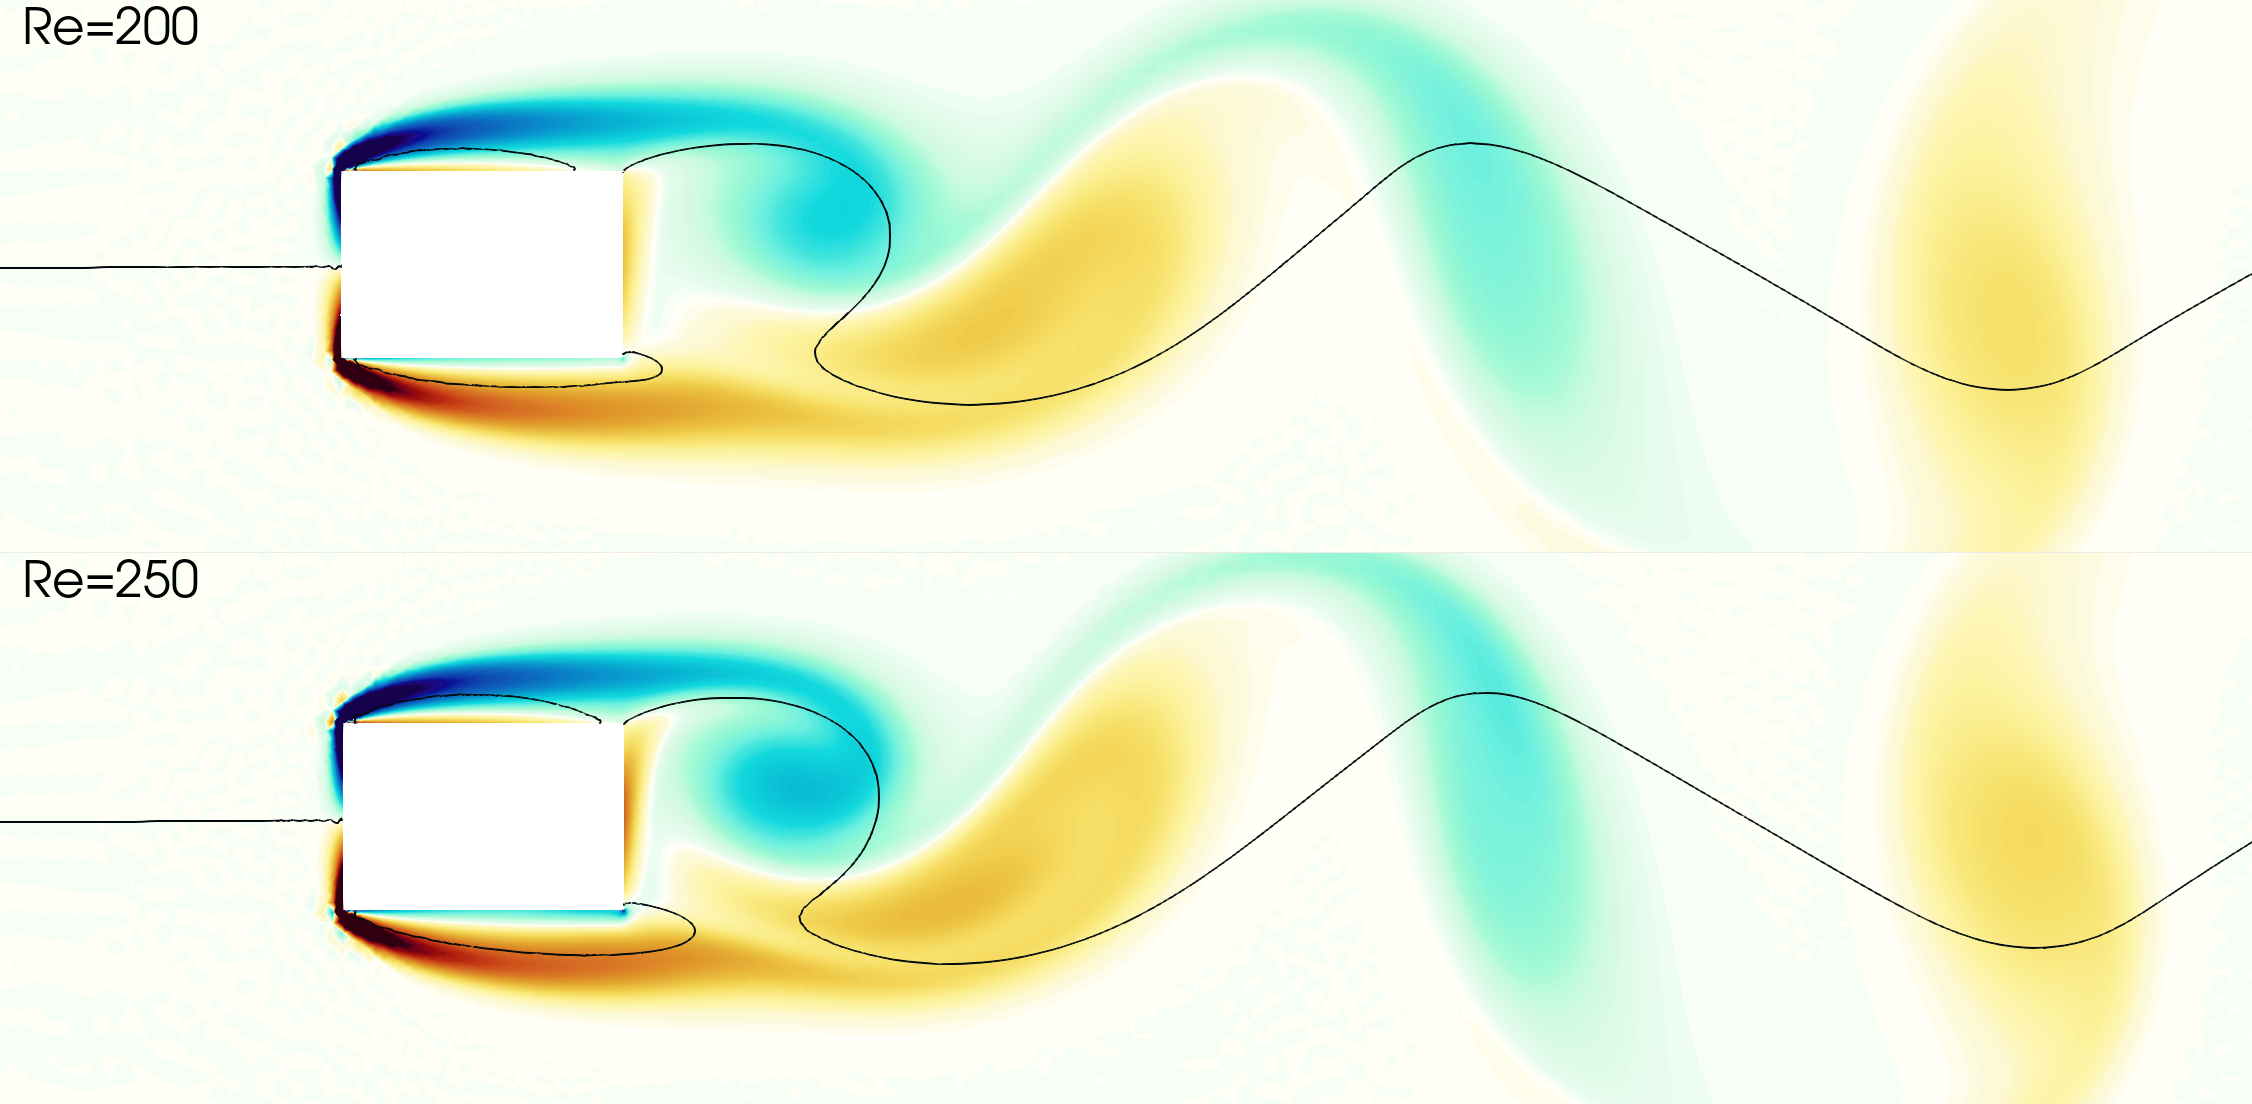
\includegraphics[width=0.49\textwidth]{./fig/AR1p5/snap/snap.0030.png}
  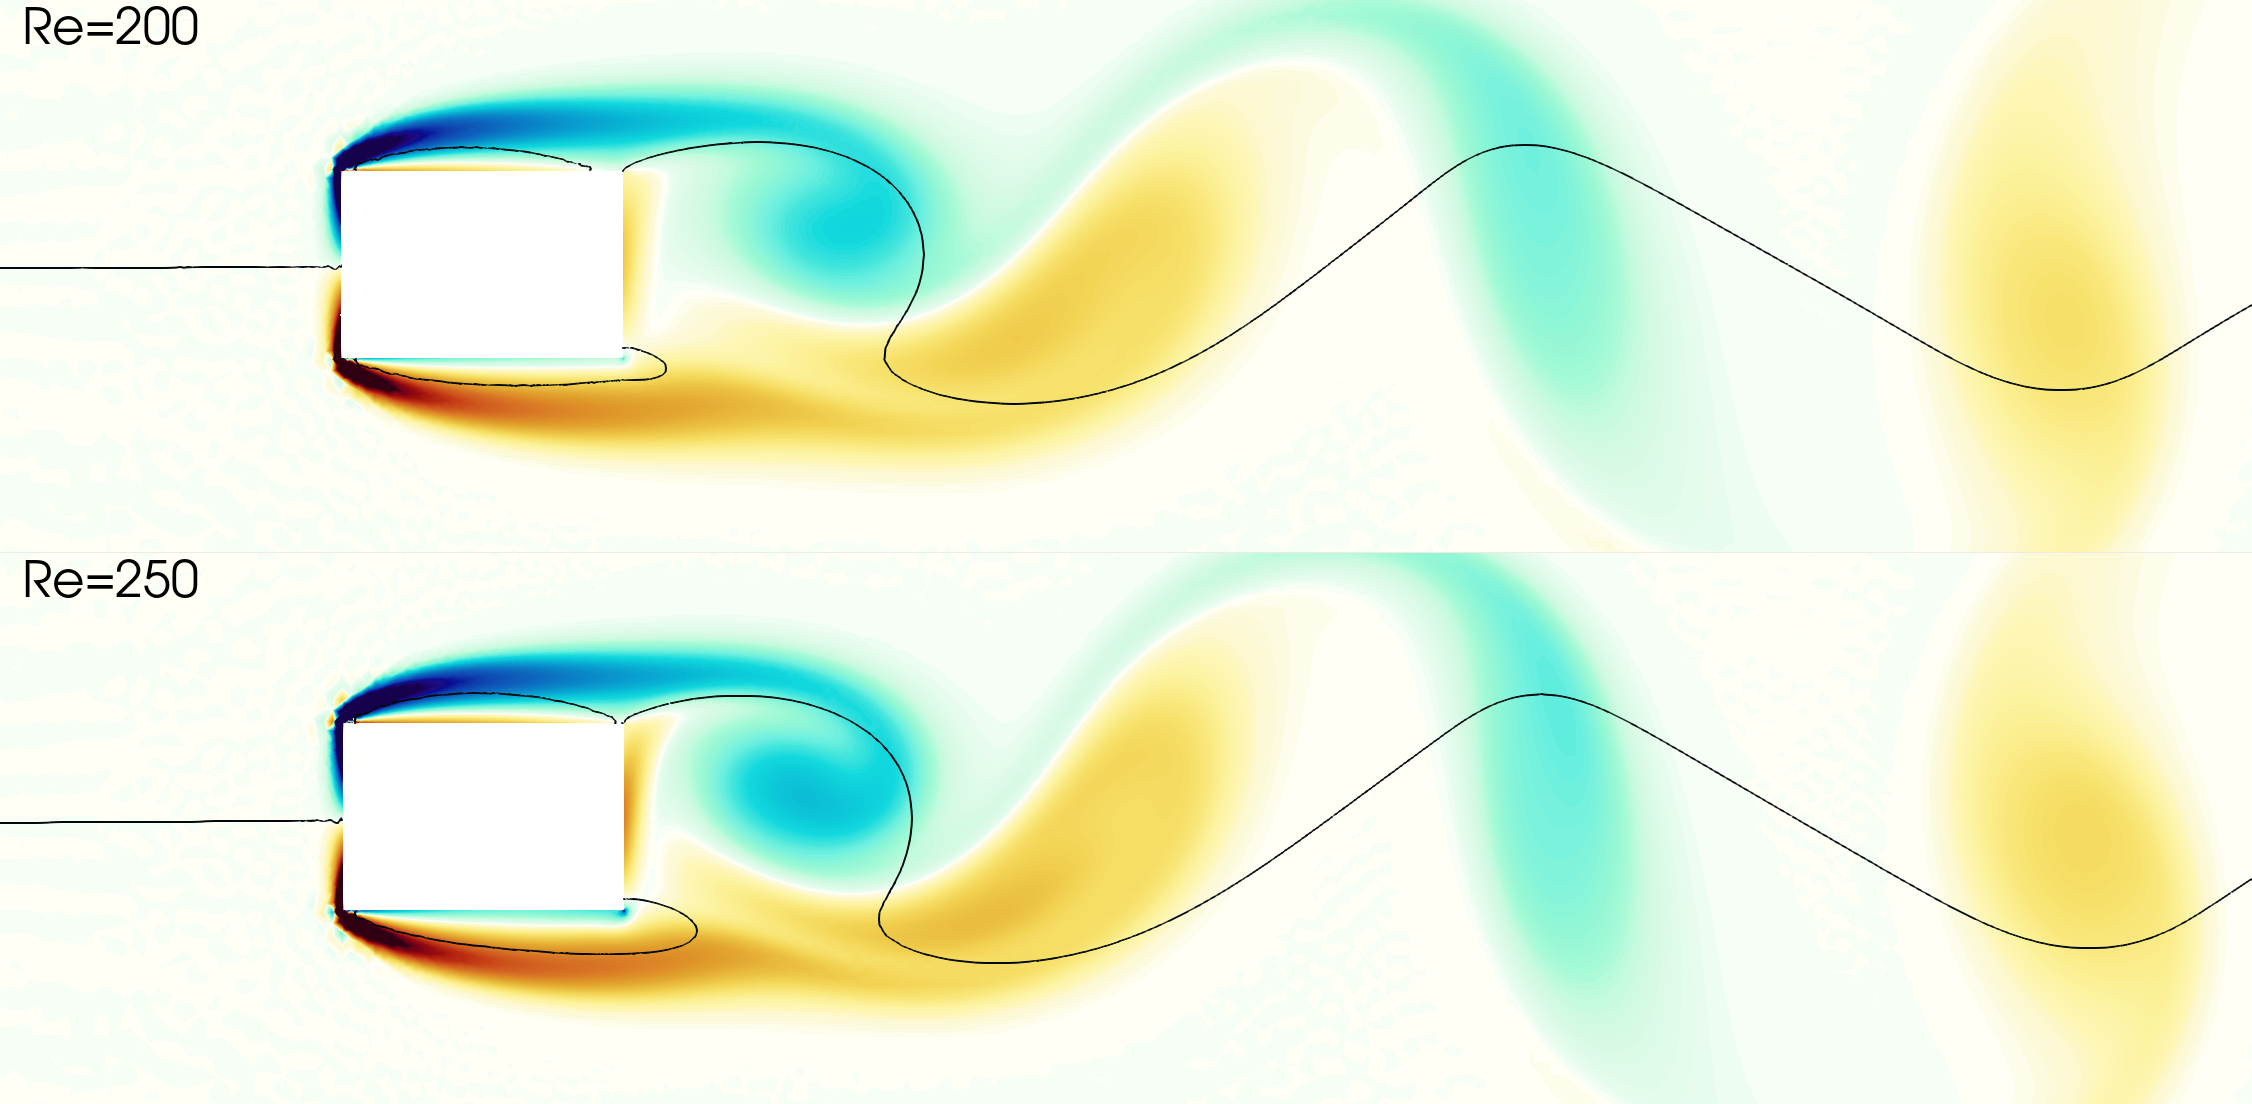
\includegraphics[width=0.49\textwidth]{./fig/AR1p5/snap/snap.0035.png}
  \begin{tikzpicture}
  \draw (-10,2) -- (8,2);
  \end{tikzpicture}
  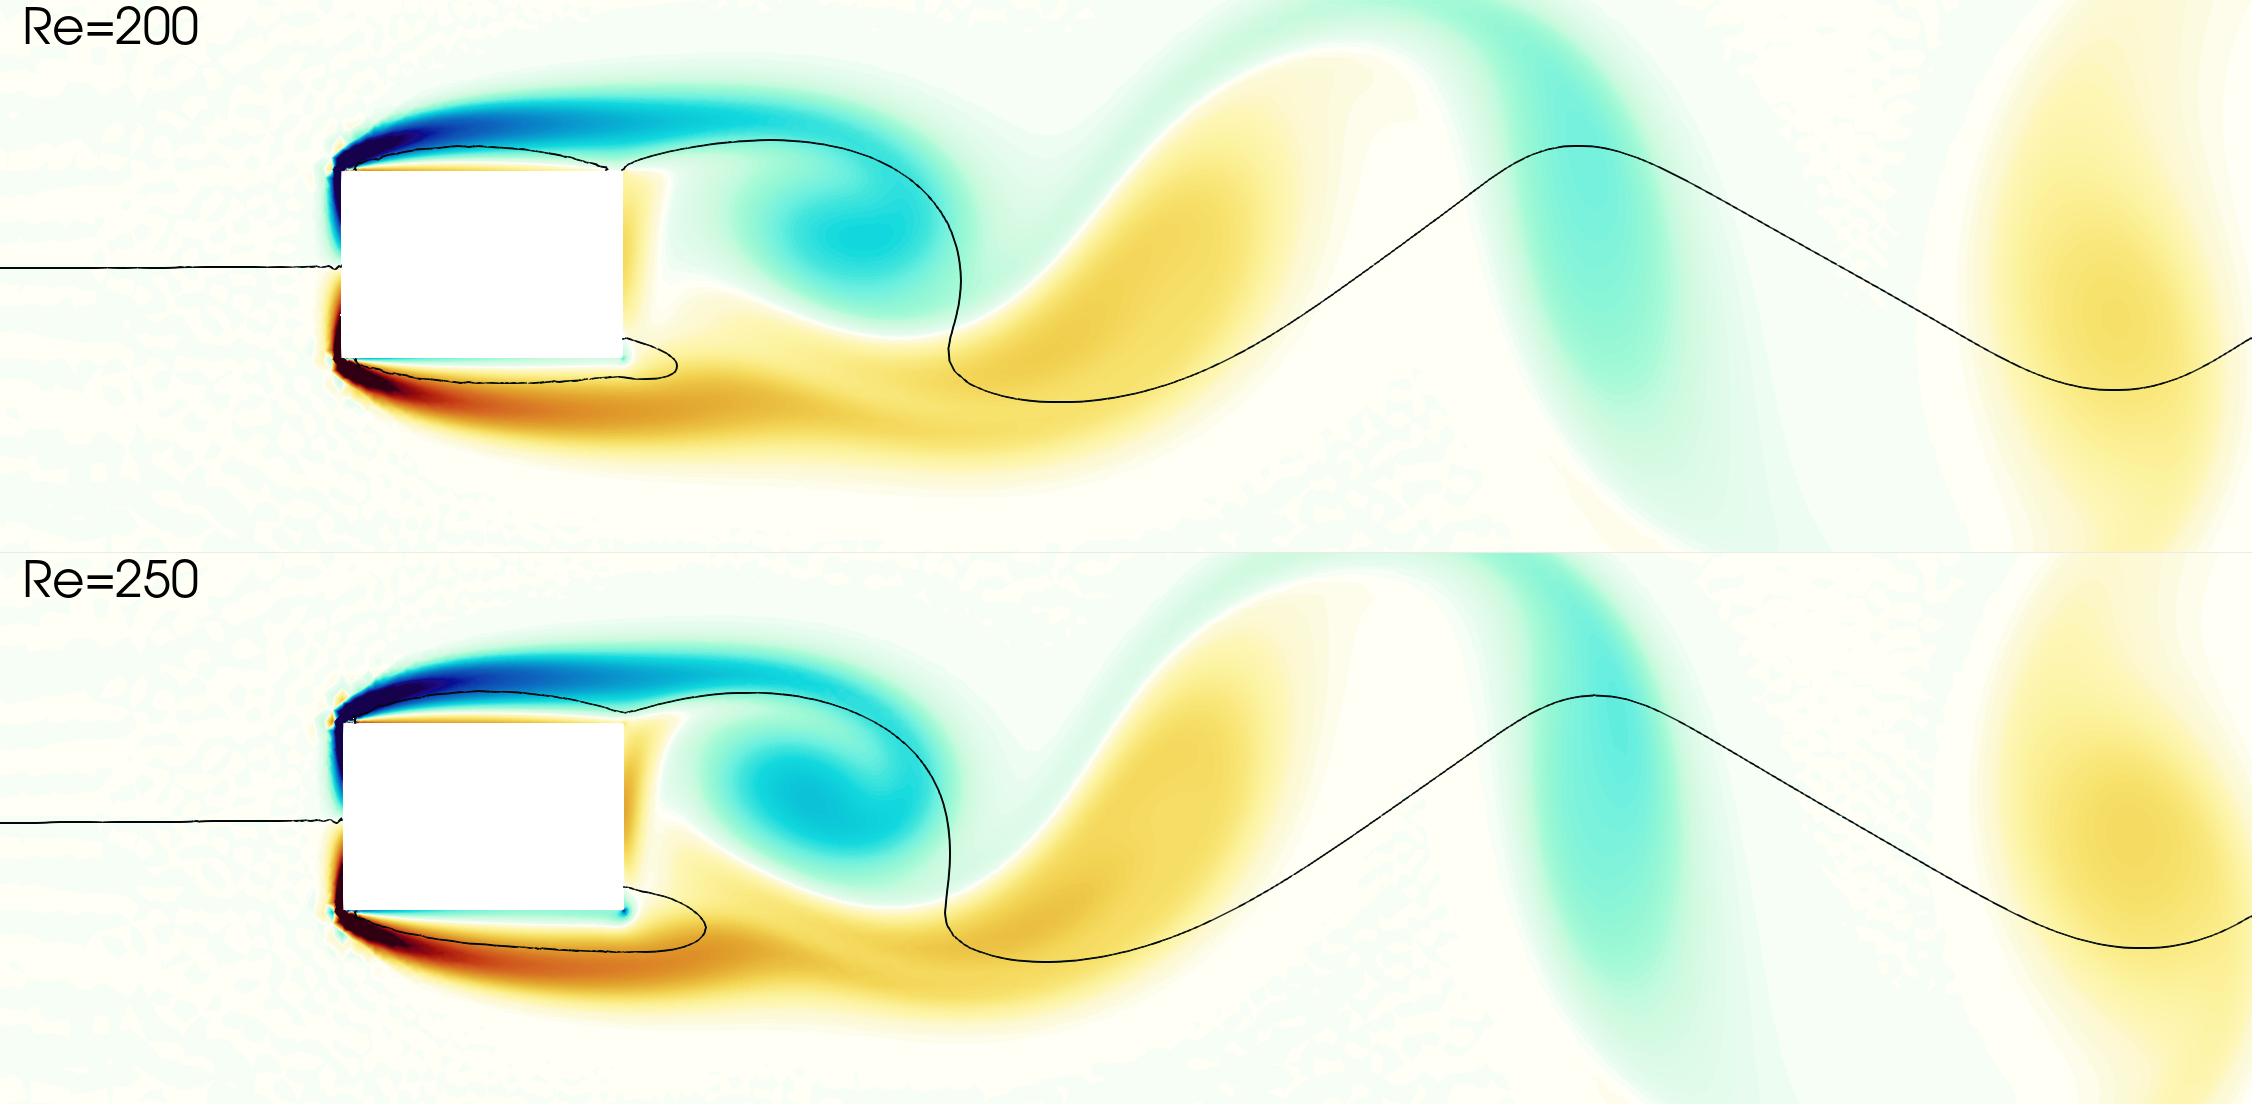
\includegraphics[width=0.49\textwidth]{./fig/AR1p5/snap/snap.0040.png}
  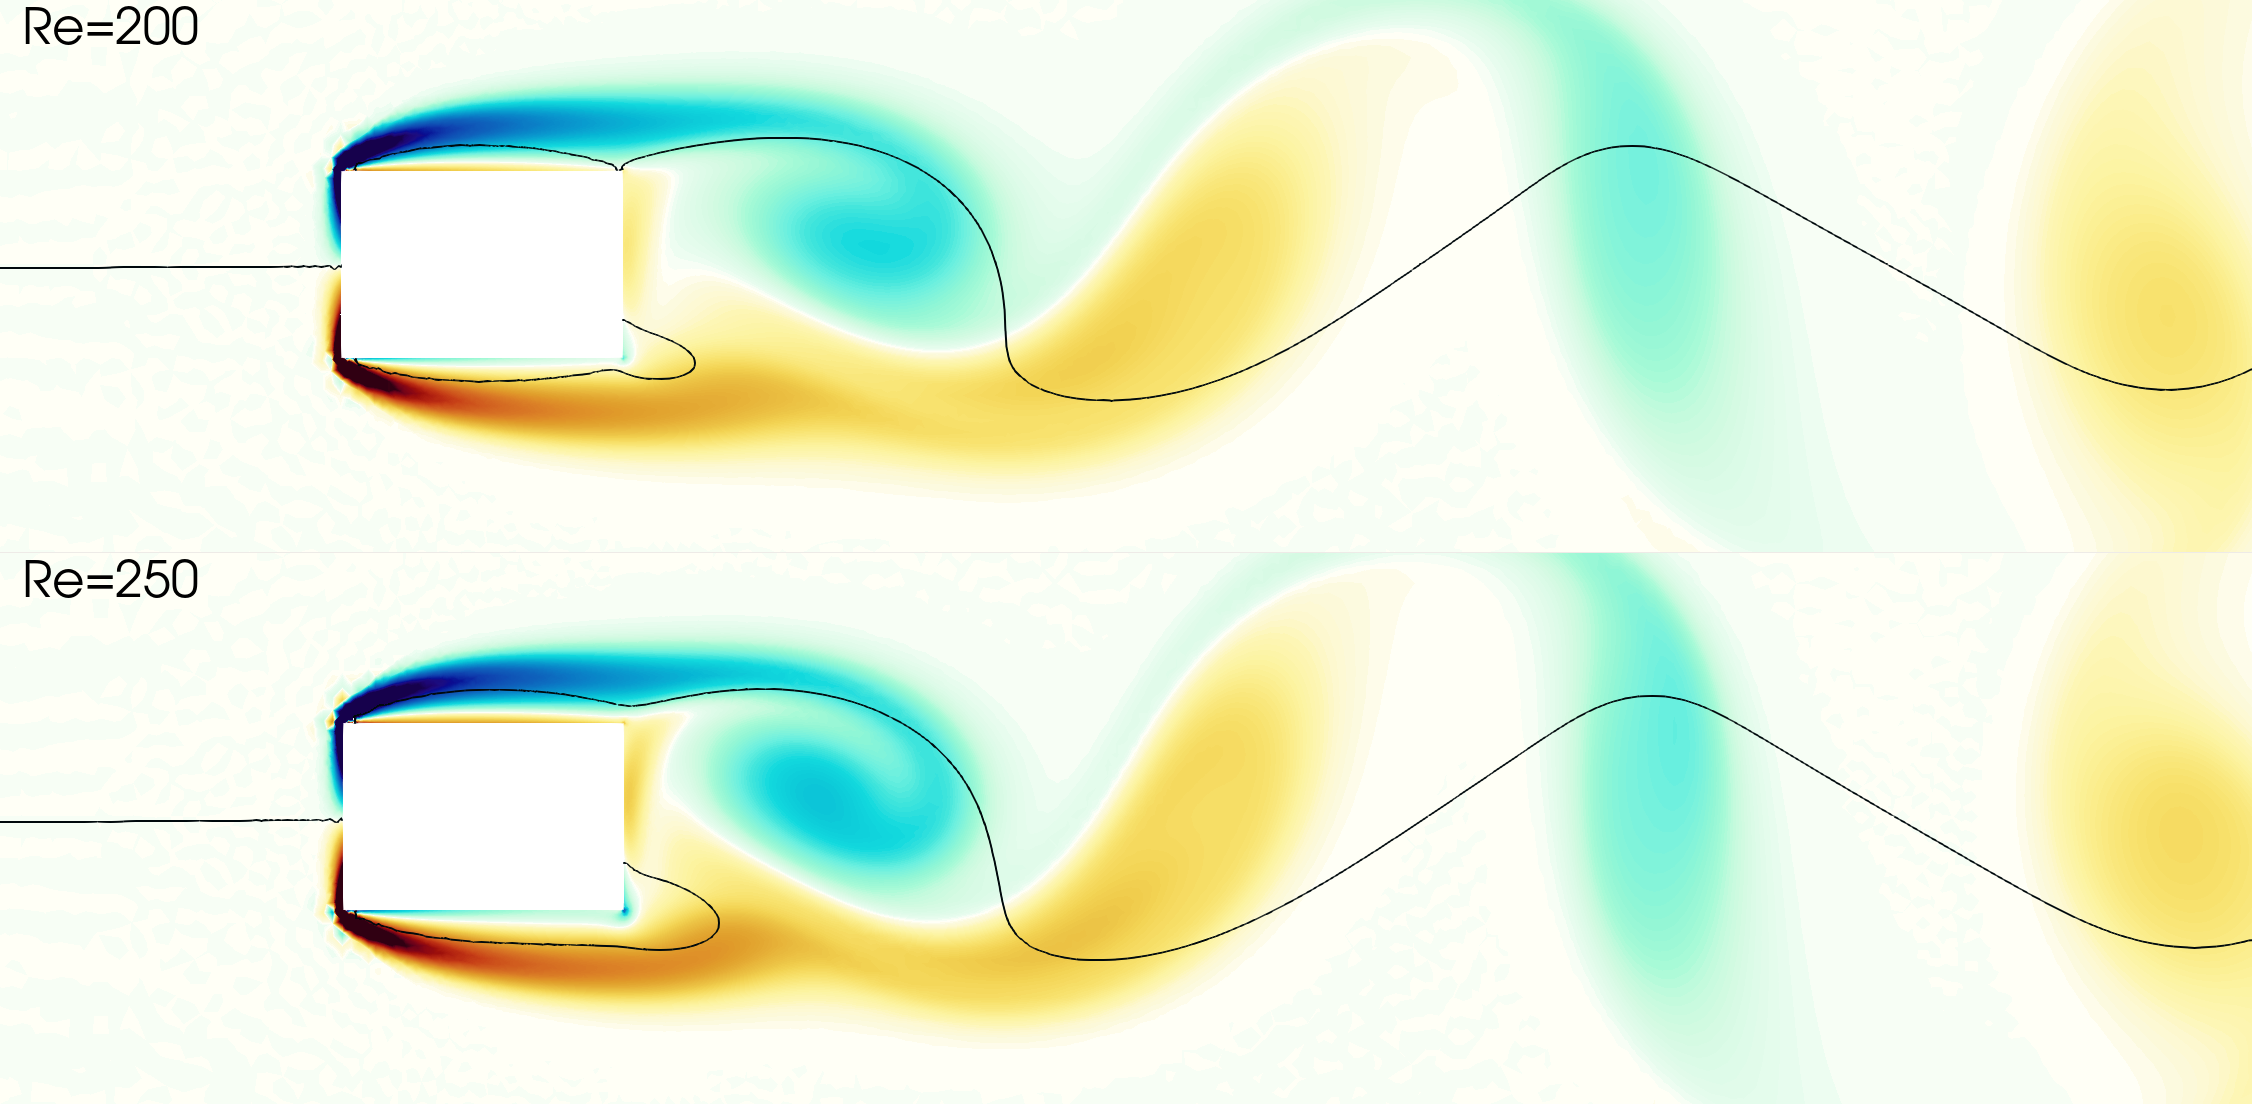
\includegraphics[width=0.49\textwidth]{./fig/AR1p5/snap/snap.0045.png}  
  \caption{$\AR=1.5$. Top: $Re=200$. Bottom: $Re=250$. Eight instantaneous snaphots takes equispaced in half of the period.}
\end{figure}  
      

\begin{figure}
  \centering
  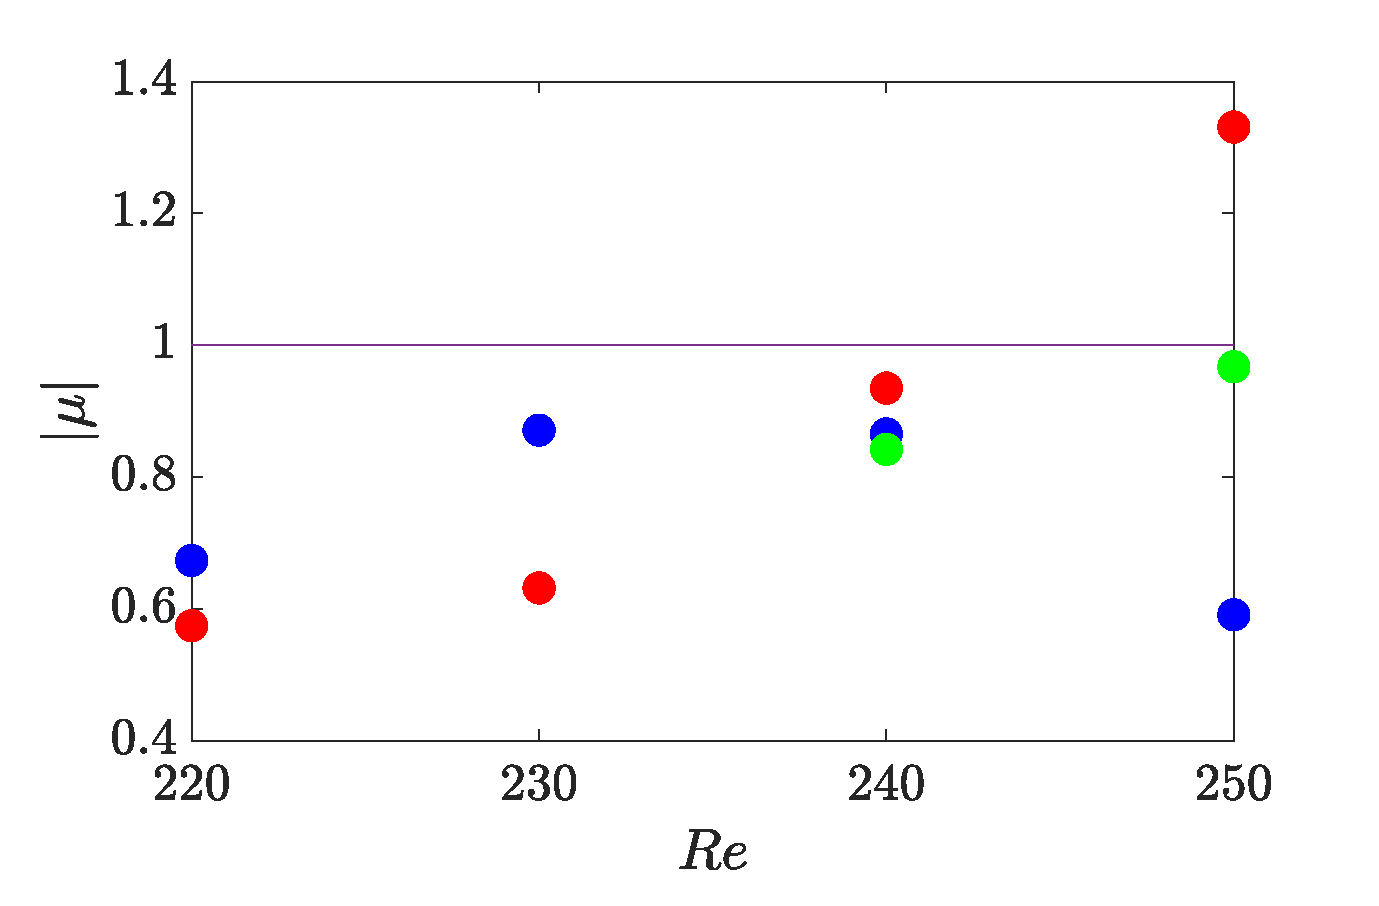
\includegraphics[width=0.49\textwidth]{./fig/AR1s/mu_Re_Ar1p25_2D.eps}
  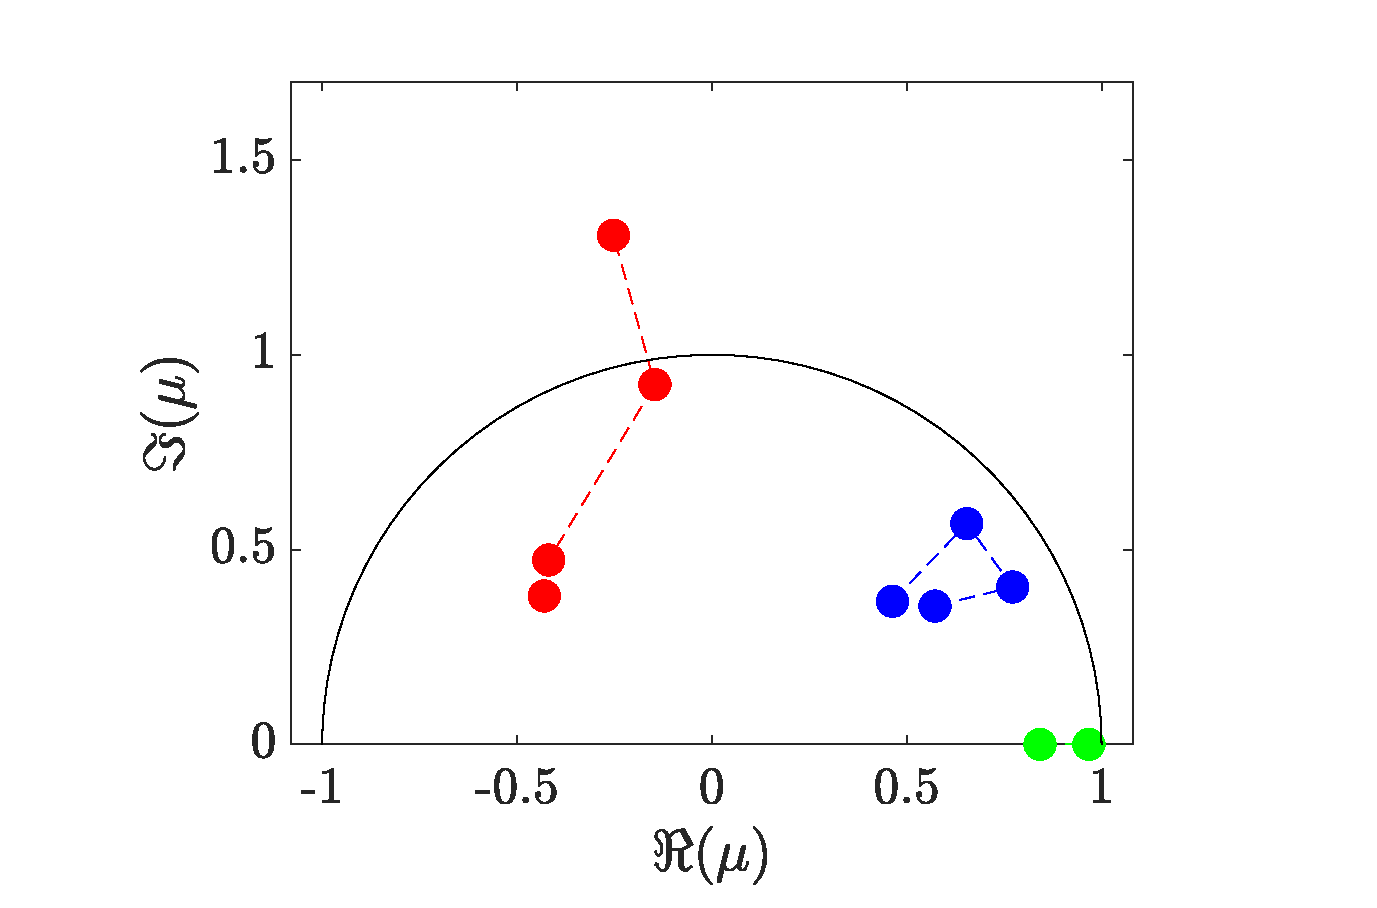
\includegraphics[width=0.49\textwidth]{./fig/AR1s/mu_Ar1p25_2D.eps}  
  \caption{Floquet multilpiers of the 2D bifurcation for $\AR=1.25$}
  \label{fig:bif2D_AR1p25}
\end{figure}

\begin{figure}
  \centering
  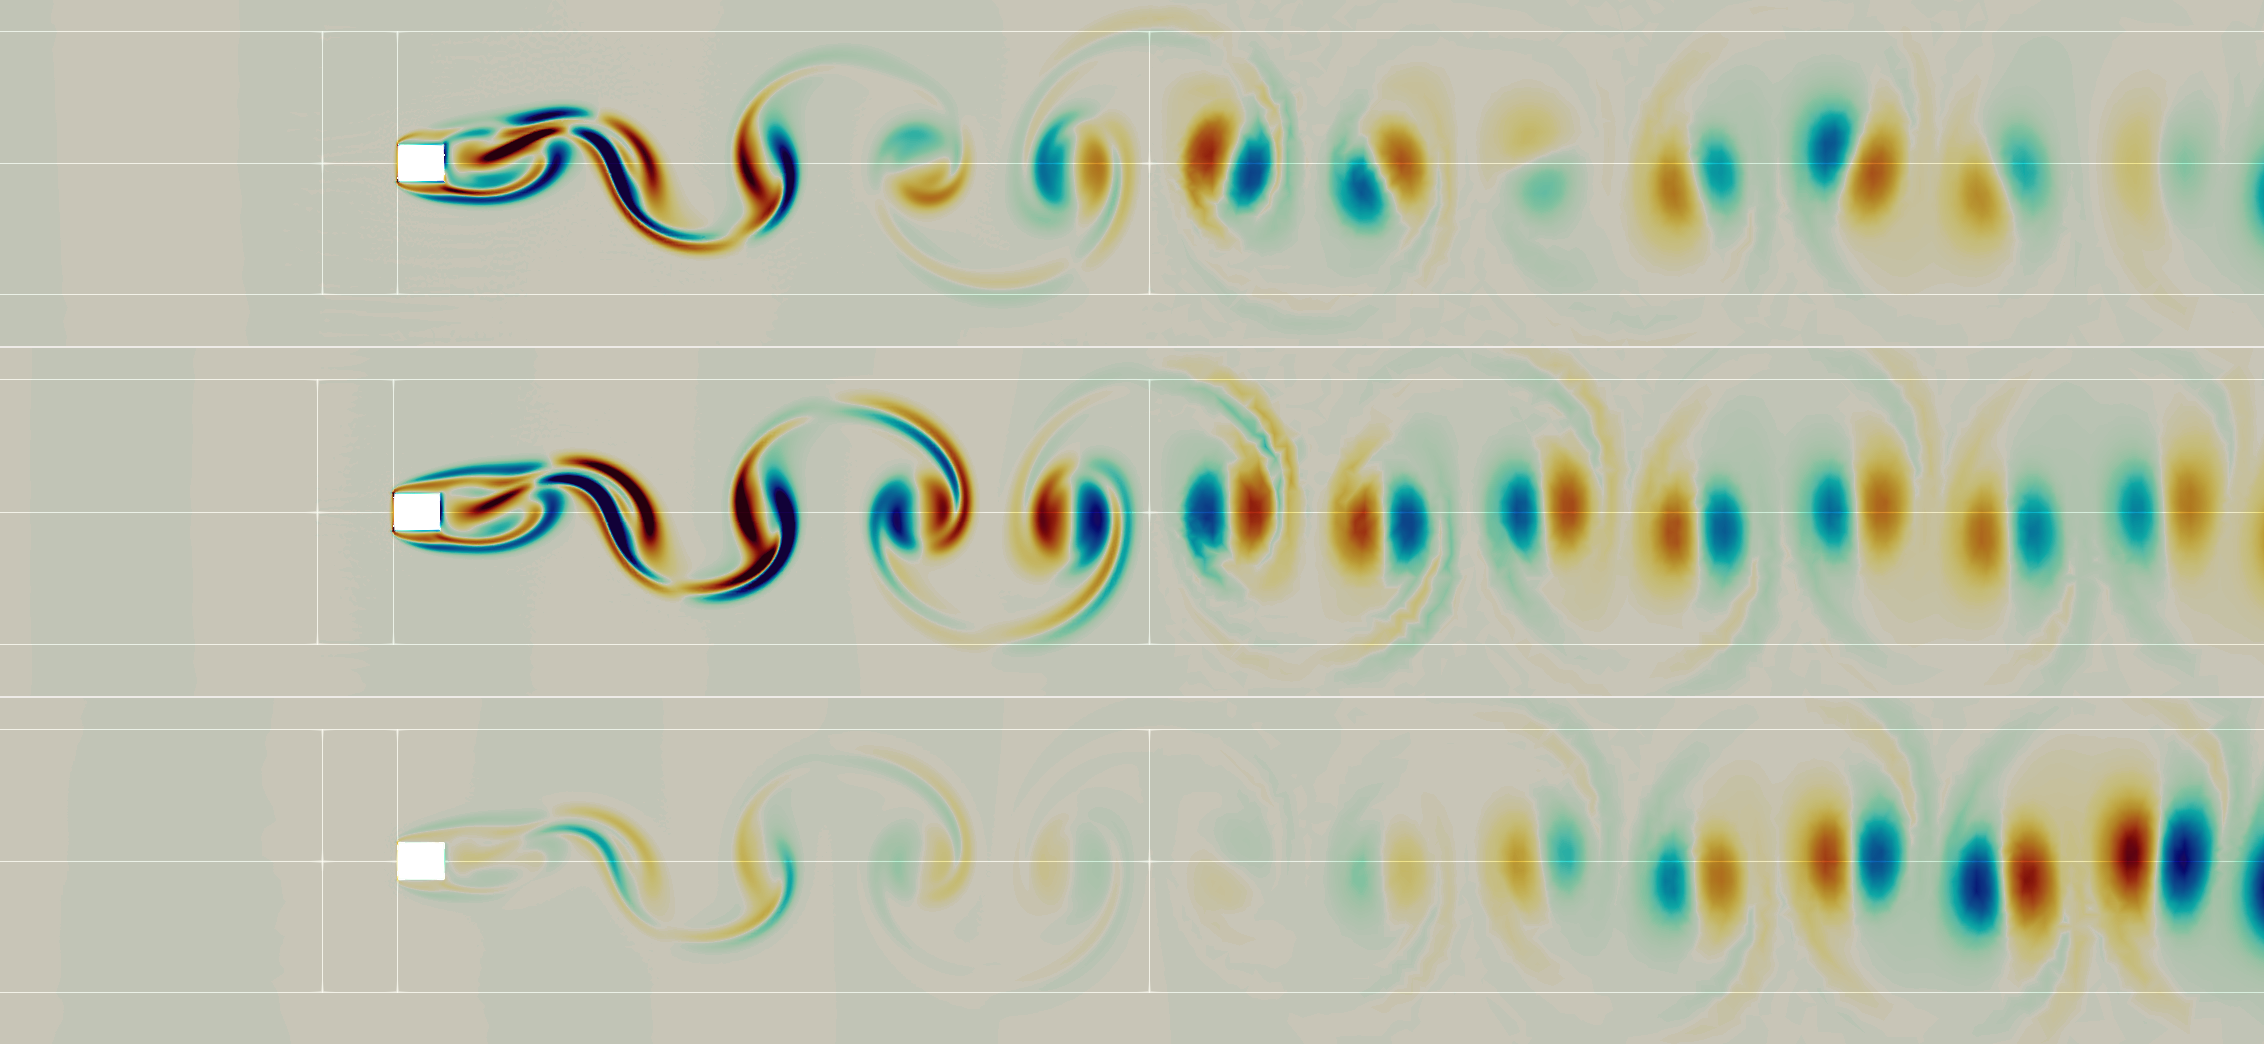
\includegraphics[width=0.7\textwidth]{./fig/AR1p25/Mode_omegar_2D_Re250.png}
  \caption{Floquet mode associated with the 2D Floquet multipliers for $Re=250$ and $\AR=1.25$. From top to bottom $|\mu|$ decreases. Referring to figure \ref{fig:bif2D_AR1p25}, the top panel refer to the red symbols, the central one to the green symbols, while the bottom panel to the blue symbols.}
  \label{fig:mod2DAR1p25}
\end{figure}

\begin{figure}
  \centering
  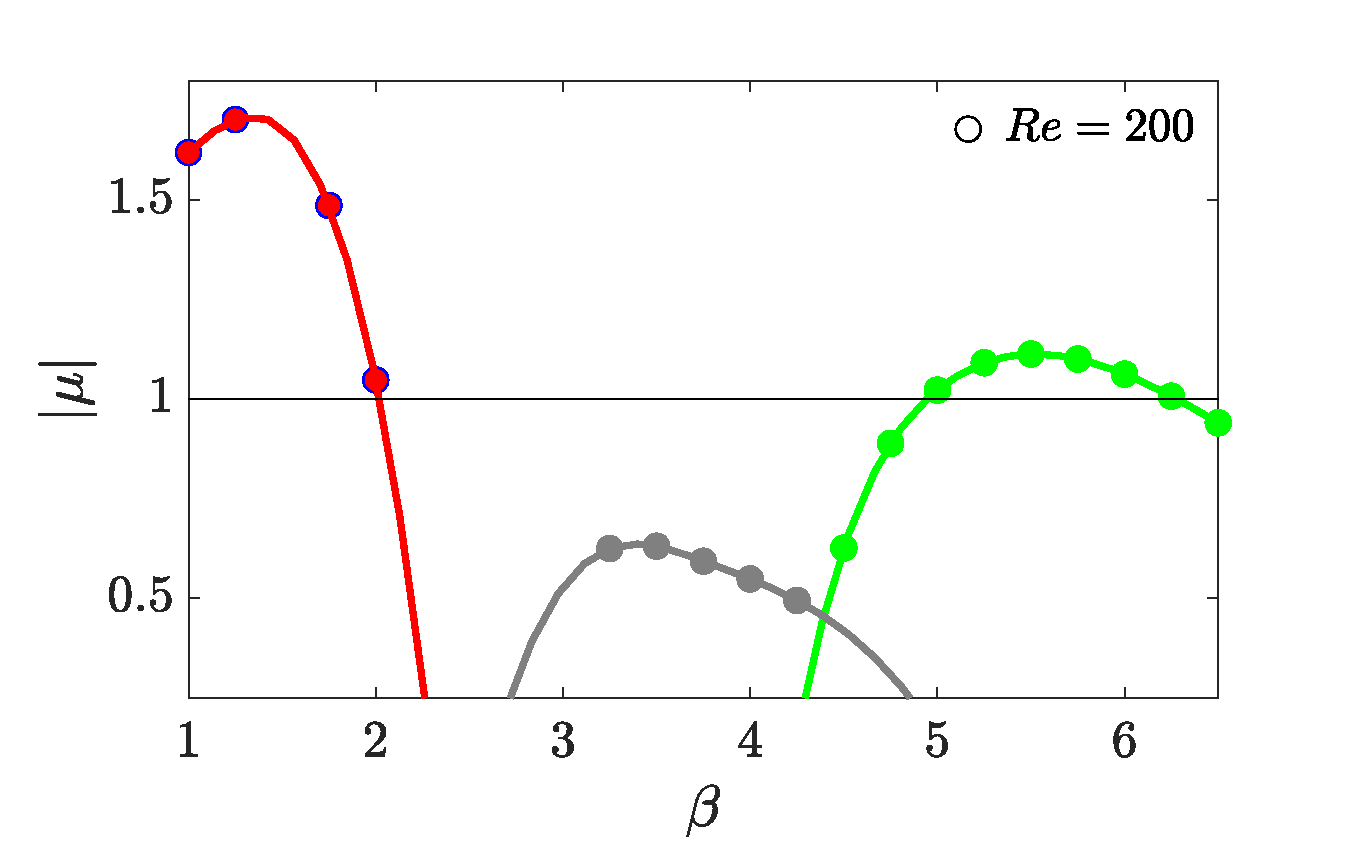
\includegraphics[width=0.49\textwidth]{./fig/AR1s/multipliers_AR1.eps}
  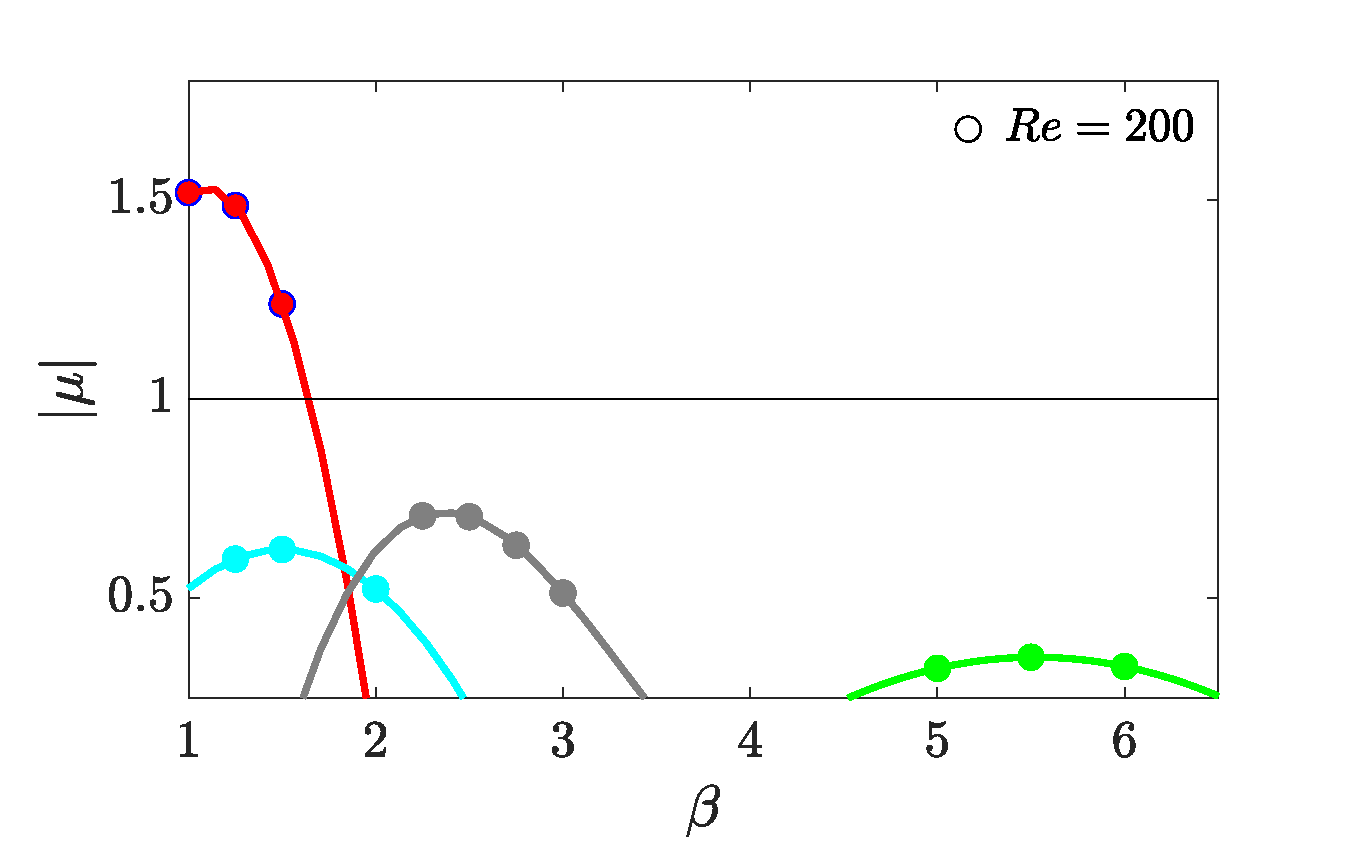
\includegraphics[width=0.49\textwidth]{./fig/AR1s/multipliers_AR1p25.eps}
  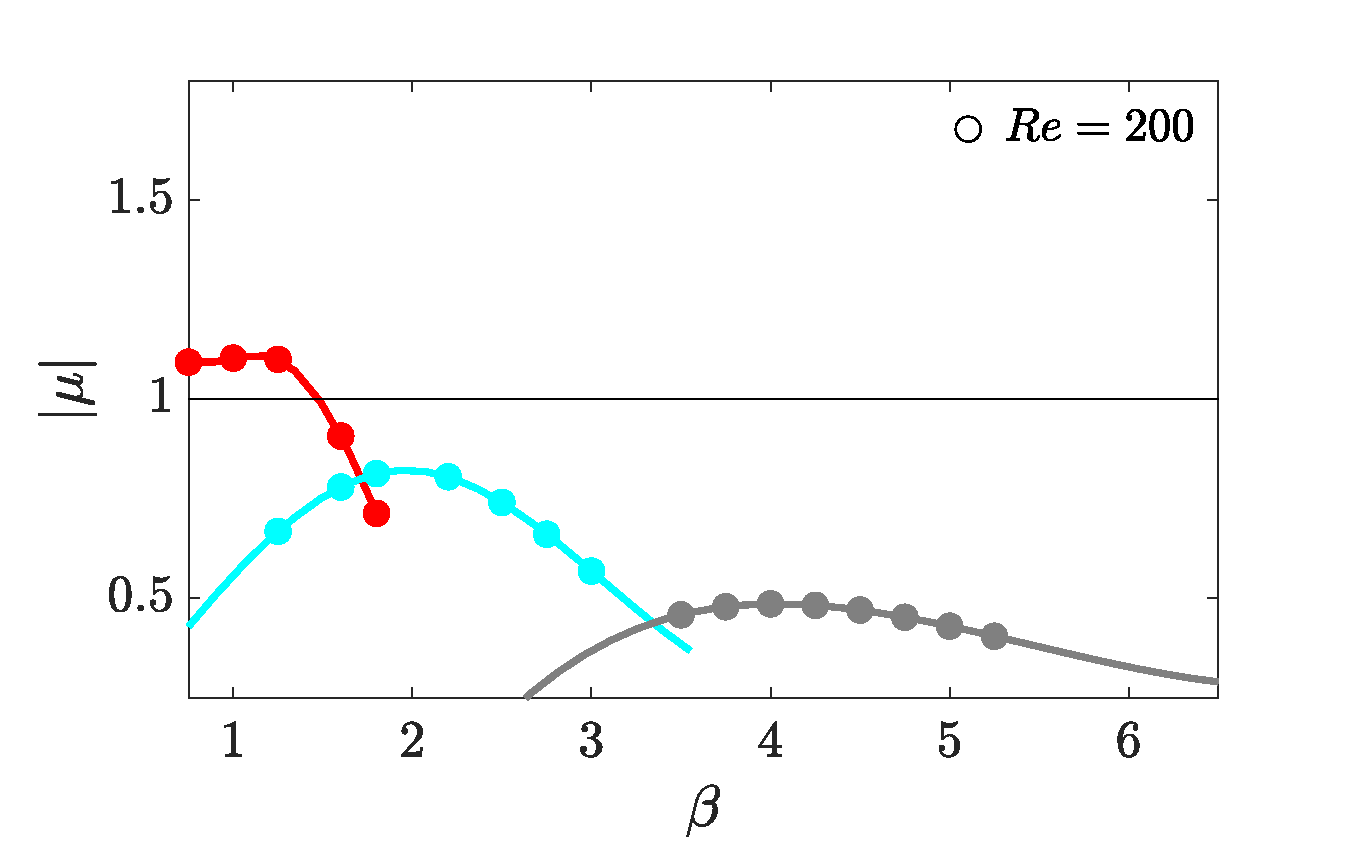
\includegraphics[width=0.49\textwidth]{./fig/AR1s/multipliers_AR1p5.eps}
  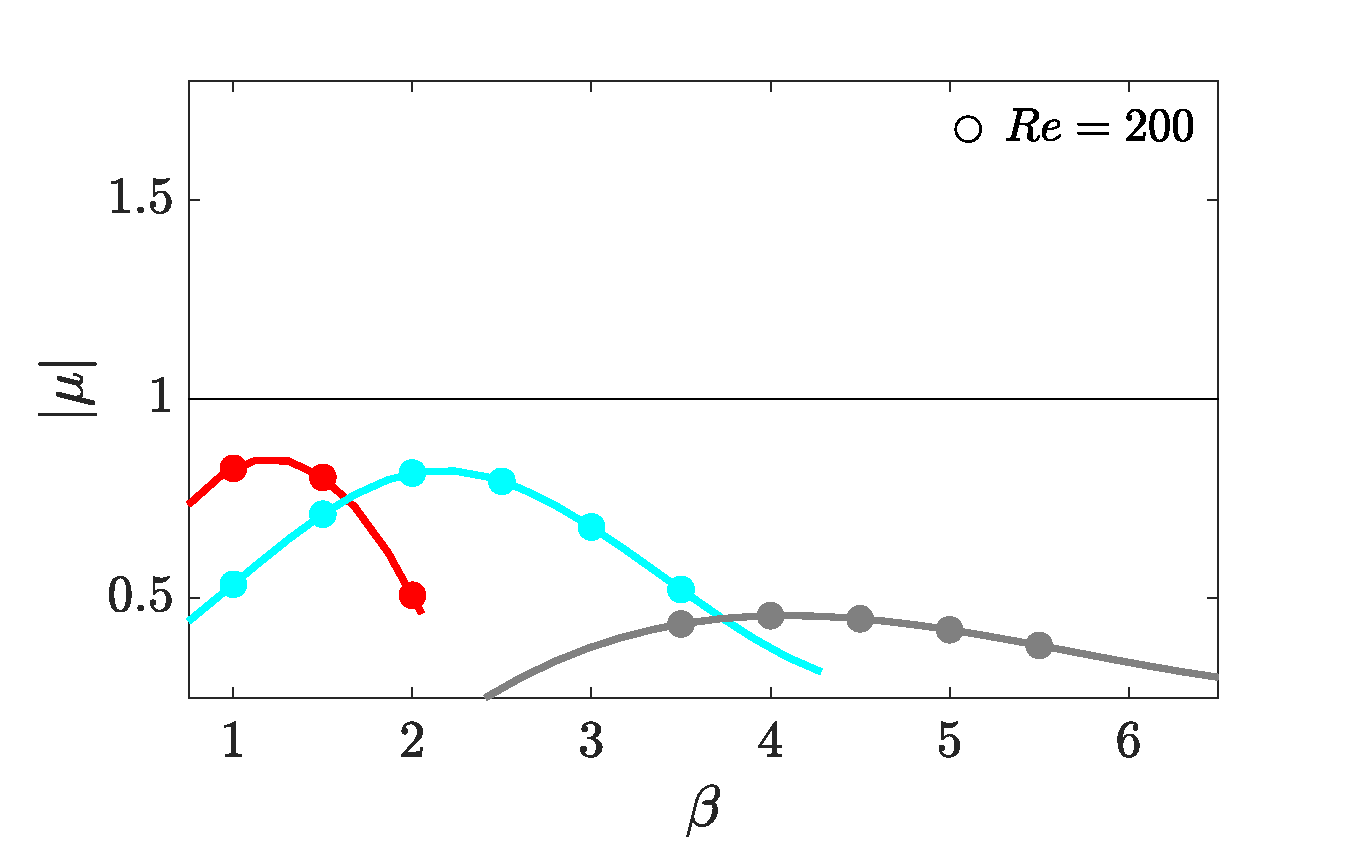
\includegraphics[width=0.49\textwidth]{./fig/AR1s/multipliers_AR1p75.eps} \\
  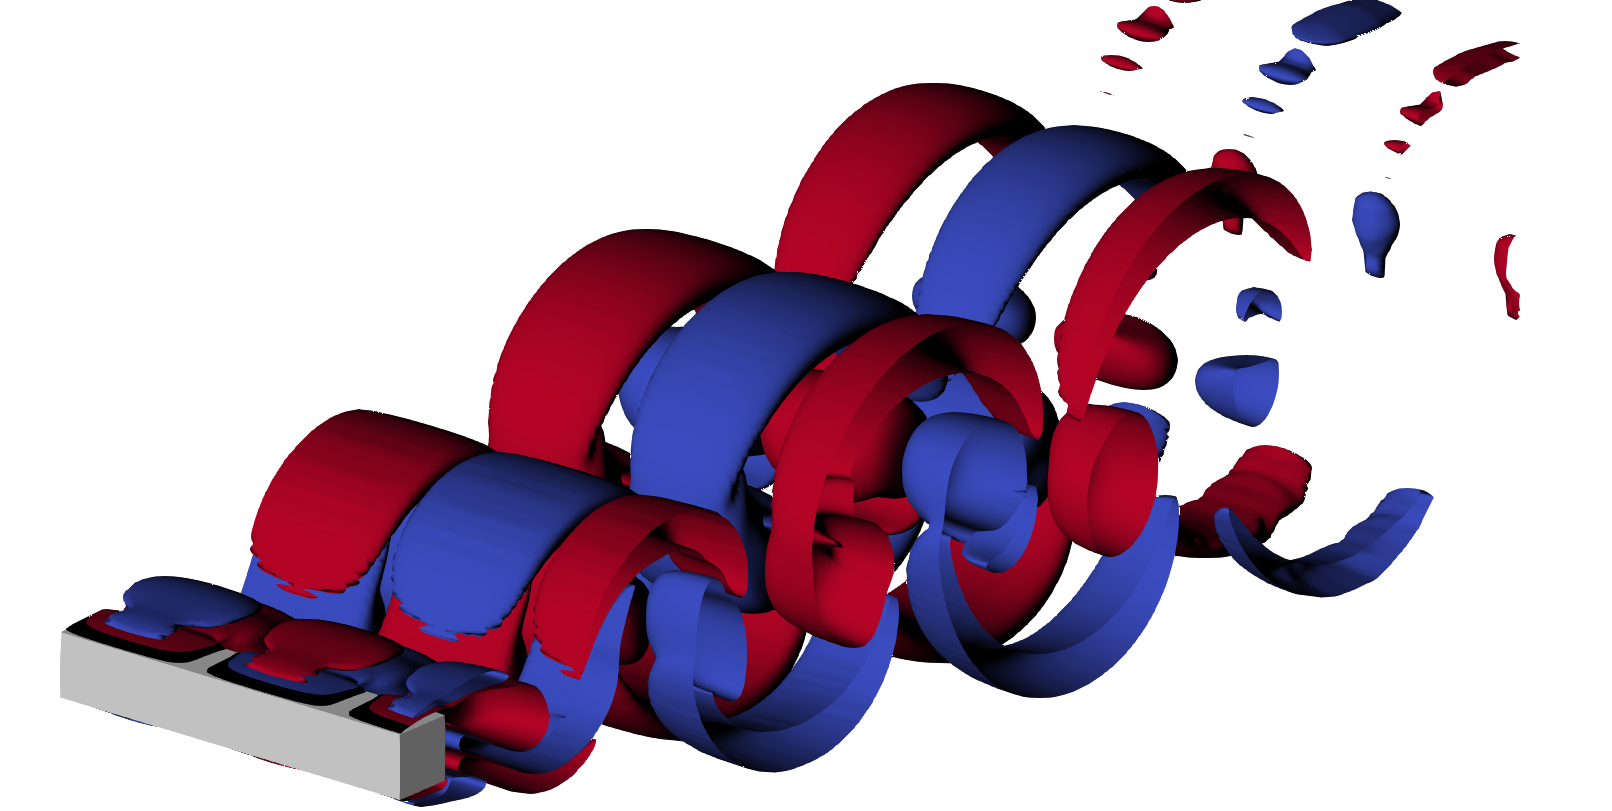
\includegraphics[width=0.32\textwidth]{./fig/AR1s/Floqetmode_beta_1p2_Re200_AR1_A.png}
  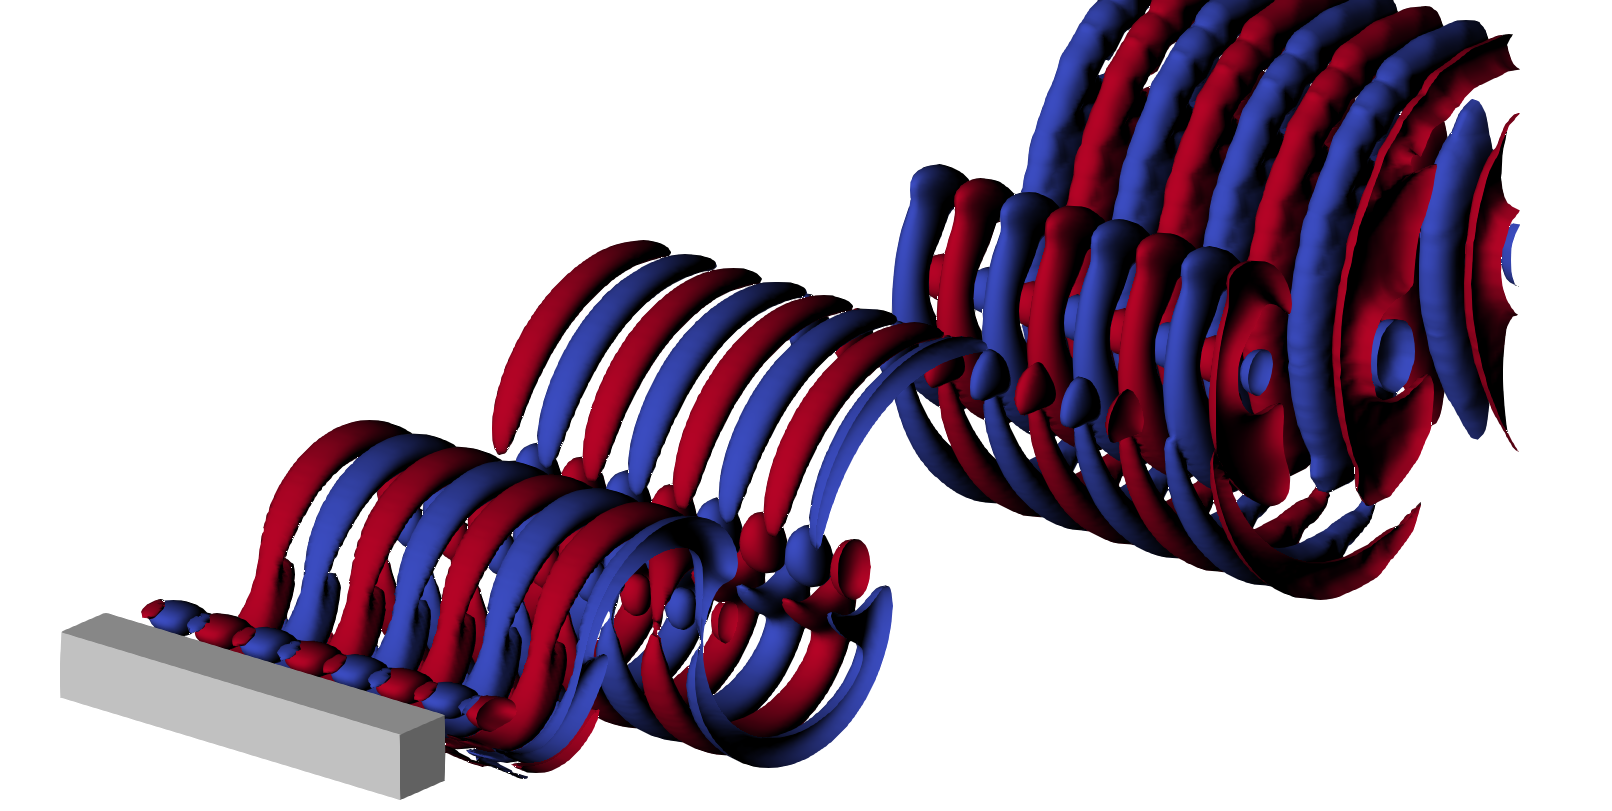
\includegraphics[width=0.32\textwidth]{./fig/AR1s/Floqetmode_beta_3p75_Re200_AR1_C.png}      
  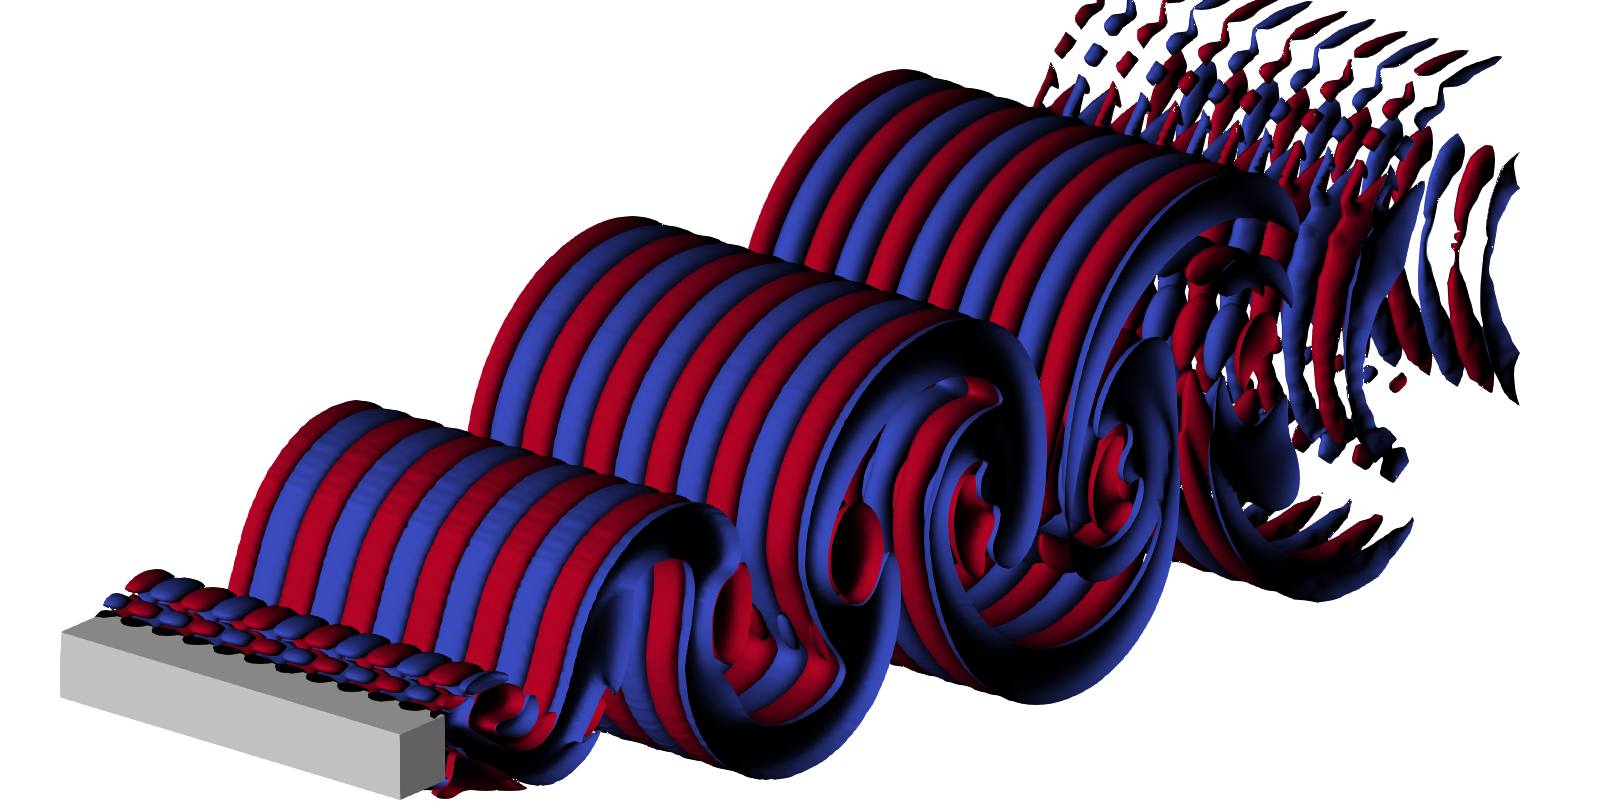
\includegraphics[width=0.32\textwidth]{./fig/AR1s/Floqetmode_beta_5p5_Re200_AR1_B.png}
  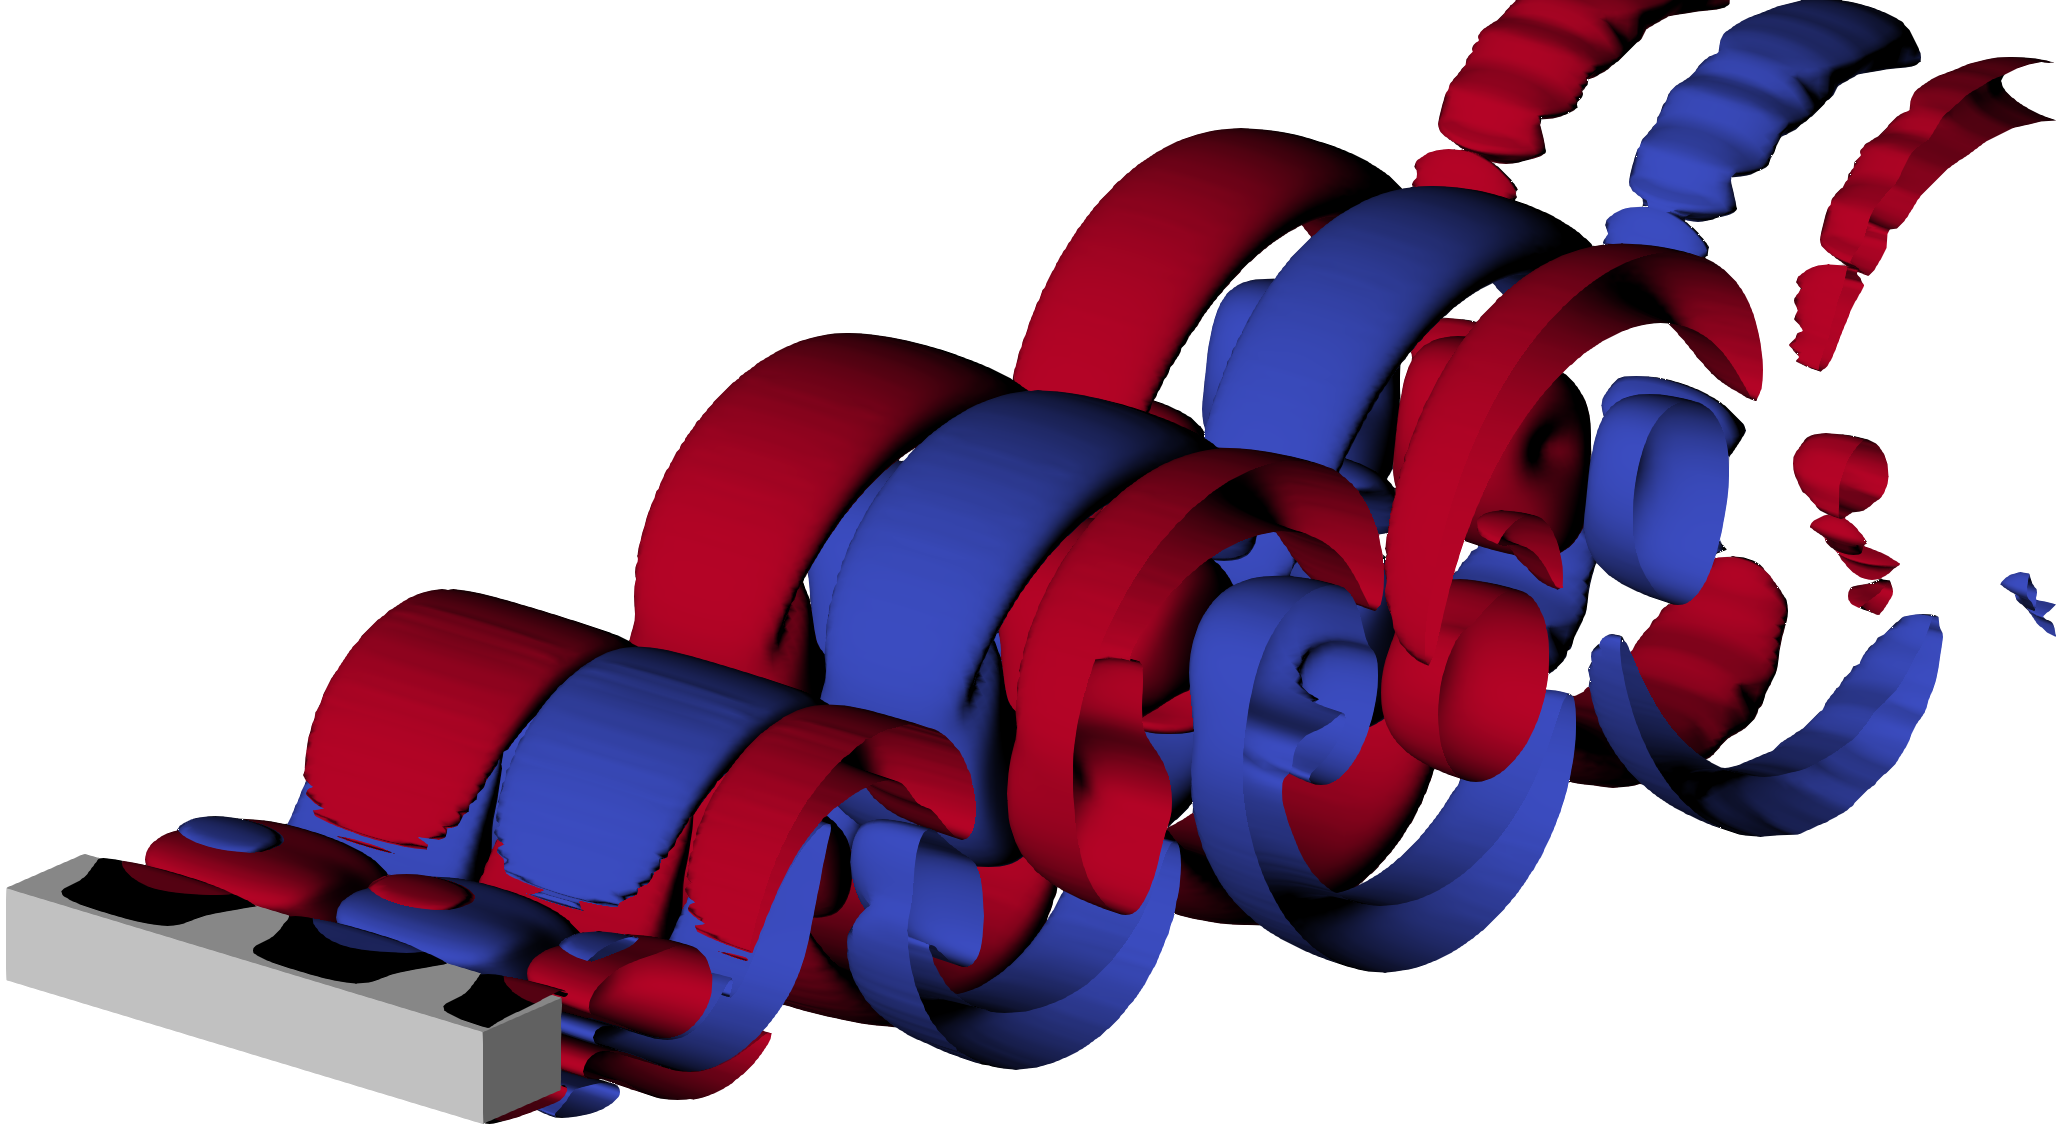
\includegraphics[width=0.32\textwidth]{./fig/AR1s/Floqetmode_beta_1p25_Re200_AR1p25_A.png}
  \includegraphics[width=0.32\textwidth]{./fig/AR1s/Floqetmode_beta_1p25_Re200_AR1p25_Bp.png}
  \includegraphics[width=0.32\textwidth]{./fig/AR1s/Floqetmode_beta_5p5_Re200_AR1p25_B.png}
  \includegraphics[width=0.32\textwidth]{./fig/AR1s/Floqetmode_beta_1p8_Re200_AR1p5_A.png}
  \includegraphics[width=0.32\textwidth]{./fig/AR1s/Floqetmode_beta_1p8_Re200_AR1p5_Bp.png}
  \includegraphics[width=0.32\textwidth]{./fig/AR1s/Floqetmode_beta_3p75_Re200_AR1p5_C.png}
  \caption{Top: multipliers for $\AR=1$, $\AR=1.25$ and $\AR=1.5$ at $Re=200$; the red line refers to mode $A$, the grey line to mode $C$, the green line to mode $B$ and the light blue line refers to mode $B'$. Mode $B'$ has the same spatio-temporal symmetry of mode $B$, but its characteristic wavelength is much smaller, being similar to that of mode $A$. This mode resembles that found for elongated bodies with elliptic leading edge by \cite{ryan-etal-2005}. The bottom panels show the Floquet modes associated with the different branches for the three $\AR$s. Top: Floquet modes for $\AR=1$ and $Re=200$, associated with mode A (left, $\beta=1.2$), mode C (centre, $\beta=3.75$) and mode $B$ (right, $\beta=5.5$). Centre: Floquet modes for $\AR=1.25$ and $Re=200$ associated with mode A (left, $\beta=1.25$), mode $B'$ (centre, $\beta = 1.25$) and mode $B$ (right, $\beta=5.5$). Bottom: Floquet modes for $\AR=1.5$ and $Re=200$ associated with mode A (left, $\beta=1.8$), mode $B'$ (centre, $\beta=1.8$) and mode $C$ (right, $\beta=3.75$). These are 3D reconstructions of the Floquet modes and the red/blue isosurfaces denote positive/negative streamwise vorticity. XX ADD $Re=175$ FOR ALL CASES XX}
  \label{fig:xx}
\end{figure}


\begin{figure}
  \centering
  \includegraphics[width=0.49\textwidth]{./fig/AR1p25/mu_beta_Re210.eps}
  \includegraphics[width=0.49\textwidth]{./fig/AR1p25/mu_beta_Re220.eps}
  \includegraphics[width=0.49\textwidth]{./fig/AR1p25/mu_beta_Re230.eps}
  \includegraphics[width=0.49\textwidth]{./fig/AR1p25/mu_beta_Re240.eps}
  \includegraphics[width=0.49\textwidth]{./fig/AR1p25/mu_beta_Re250.eps}
  \caption{Modulus of the Floquet multipliers for $\AR=1.25$ at different $Re$. In order, the panels are for $Re=210$, $Re=220$, $Re=230$, $Re=240$ and $Re=250$. Red colour is for real and positive multipliers. Blue colour is for complex multipliers. Green colour is for real and negative multipliers. Note that for $Re=250$ at small $\beta$ we have to real, positive multipliers, associated to modes $A$ and $A'$. Then they interact and the brances collapse to a new one that has non null imaginary part. Also, in this case two new mode of subharmonic nature arise they are distinct modes, but for $\beta \approx 3$ they interact and the two branches collapse to a unique one. Then they separate again. XX ADD THE MODES XX}
\end{figure}

\begin{figure}
  \centering
  \includegraphics[width=0.49\textwidth]{./fig/AR1p25/omegax_Re230_beta_2p25_modeC.eps}
  \includegraphics[width=0.49\textwidth]{./fig/AR1p25/omegax_Re230_beta_2p25_modeD.eps}
  \includegraphics[width=0.49\textwidth]{./fig/AR1p25/omegax_Re240_beta_0p5_modeBpp.eps}
  \includegraphics[width=0.49\textwidth]{./fig/AR1p25/omegax_Re250_beta_1_modeAp.eps}
  \includegraphics[width=0.49\textwidth]{./fig/AR1p25/omegax_Re250_beta_3_modeS.eps}
  \includegraphics[width=0.49\textwidth]{./fig/AR1p25/omegax_Re250_beta_3_modeSp.eps}
  \caption{Imaginary part of the streamwise vorticity of the Floquet modes for $\AR=1.25$. Top left: mode $C$ for $Re=230$, $\beta=2.25$. Top right: mode $D$ for $Re=230$, $\beta=2.25$. Centre left: mode $B'$ for $Re=240$ and $beta=0.5$. Centre right: mode $A'$ for $Re=250$ and $\beta=3$. Bottom left: mode $S$ for $Re=250$ and $\beta=3$. Bottom right: mode $S'$ for $Re=250$ and $\beta=3$.}
  \label{fig:modes_AR1p25}
\end{figure}


\begin{itemize}
  \item In this subsection we look at $\AR \in (1,2)$.
  \item Brifely recall the bifurcation scenario that has been observed for $\AR=1$, i.e. modes $A$, $QP$ and $B$.
  \item Give evidence of the influence of $\AR$ on these modes. They indeed stabilise a $\AR$ increases. Mode $B$ is not present any more for $\AR>1.25$. A new mode arises.
  \item Look at the symmetries of the modes.  
  \item \textcolor{blue}{For $\AR=1.25$ and $\AR=1.5$, modes $A$ and $B'$ become unstable is short succession. We can so use DNS to see what happens as $Re$ increases, and whether the flow changes from one mode to the other. (POD?)}
  \item Maybe we should add also $\AR=2$ and $\AR=2.5$ to see what happens.
\end{itemize}
